% Generated by Sphinx.
\def\sphinxdocclass{report}
\documentclass[letterpaper,10pt,english]{sphinxmanual}
\usepackage[utf8]{inputenc}
\DeclareUnicodeCharacter{00A0}{\nobreakspace}
\usepackage[T1]{fontenc}
\usepackage{babel}
\usepackage{times}
\usepackage[Bjarne]{fncychap}
\usepackage{longtable}
\usepackage{sphinx}
\usepackage{epstopdf}

\title{mwavepy Documentation}
\date{October 10, 2011}
\release{1.4}
\author{alex arsenovic}
\newcommand{\sphinxlogo}{}
\renewcommand{\releasename}{Release}
\makeindex

\makeatletter
\def\PYG@reset{\let\PYG@it=\relax \let\PYG@bf=\relax%
    \let\PYG@ul=\relax \let\PYG@tc=\relax%
    \let\PYG@bc=\relax \let\PYG@ff=\relax}
\def\PYG@tok#1{\csname PYG@tok@#1\endcsname}
\def\PYG@toks#1+{\ifx\relax#1\empty\else%
    \PYG@tok{#1}\expandafter\PYG@toks\fi}
\def\PYG@do#1{\PYG@bc{\PYG@tc{\PYG@ul{%
    \PYG@it{\PYG@bf{\PYG@ff{#1}}}}}}}
\def\PYG#1#2{\PYG@reset\PYG@toks#1+\relax+\PYG@do{#2}}

\def\PYG@tok@gd{\def\PYG@tc##1{\textcolor[rgb]{0.63,0.00,0.00}{##1}}}
\def\PYG@tok@gu{\let\PYG@bf=\textbf\def\PYG@tc##1{\textcolor[rgb]{0.50,0.00,0.50}{##1}}}
\def\PYG@tok@gt{\def\PYG@tc##1{\textcolor[rgb]{0.00,0.25,0.82}{##1}}}
\def\PYG@tok@gs{\let\PYG@bf=\textbf}
\def\PYG@tok@gr{\def\PYG@tc##1{\textcolor[rgb]{1.00,0.00,0.00}{##1}}}
\def\PYG@tok@cm{\let\PYG@it=\textit\def\PYG@tc##1{\textcolor[rgb]{0.25,0.50,0.56}{##1}}}
\def\PYG@tok@vg{\def\PYG@tc##1{\textcolor[rgb]{0.73,0.38,0.84}{##1}}}
\def\PYG@tok@m{\def\PYG@tc##1{\textcolor[rgb]{0.13,0.50,0.31}{##1}}}
\def\PYG@tok@mh{\def\PYG@tc##1{\textcolor[rgb]{0.13,0.50,0.31}{##1}}}
\def\PYG@tok@cs{\def\PYG@tc##1{\textcolor[rgb]{0.25,0.50,0.56}{##1}}\def\PYG@bc##1{\colorbox[rgb]{1.00,0.94,0.94}{##1}}}
\def\PYG@tok@ge{\let\PYG@it=\textit}
\def\PYG@tok@vc{\def\PYG@tc##1{\textcolor[rgb]{0.73,0.38,0.84}{##1}}}
\def\PYG@tok@il{\def\PYG@tc##1{\textcolor[rgb]{0.13,0.50,0.31}{##1}}}
\def\PYG@tok@go{\def\PYG@tc##1{\textcolor[rgb]{0.19,0.19,0.19}{##1}}}
\def\PYG@tok@cp{\def\PYG@tc##1{\textcolor[rgb]{0.00,0.44,0.13}{##1}}}
\def\PYG@tok@gi{\def\PYG@tc##1{\textcolor[rgb]{0.00,0.63,0.00}{##1}}}
\def\PYG@tok@gh{\let\PYG@bf=\textbf\def\PYG@tc##1{\textcolor[rgb]{0.00,0.00,0.50}{##1}}}
\def\PYG@tok@ni{\let\PYG@bf=\textbf\def\PYG@tc##1{\textcolor[rgb]{0.84,0.33,0.22}{##1}}}
\def\PYG@tok@nl{\let\PYG@bf=\textbf\def\PYG@tc##1{\textcolor[rgb]{0.00,0.13,0.44}{##1}}}
\def\PYG@tok@nn{\let\PYG@bf=\textbf\def\PYG@tc##1{\textcolor[rgb]{0.05,0.52,0.71}{##1}}}
\def\PYG@tok@no{\def\PYG@tc##1{\textcolor[rgb]{0.38,0.68,0.84}{##1}}}
\def\PYG@tok@na{\def\PYG@tc##1{\textcolor[rgb]{0.25,0.44,0.63}{##1}}}
\def\PYG@tok@nb{\def\PYG@tc##1{\textcolor[rgb]{0.00,0.44,0.13}{##1}}}
\def\PYG@tok@nc{\let\PYG@bf=\textbf\def\PYG@tc##1{\textcolor[rgb]{0.05,0.52,0.71}{##1}}}
\def\PYG@tok@nd{\let\PYG@bf=\textbf\def\PYG@tc##1{\textcolor[rgb]{0.33,0.33,0.33}{##1}}}
\def\PYG@tok@ne{\def\PYG@tc##1{\textcolor[rgb]{0.00,0.44,0.13}{##1}}}
\def\PYG@tok@nf{\def\PYG@tc##1{\textcolor[rgb]{0.02,0.16,0.49}{##1}}}
\def\PYG@tok@si{\let\PYG@it=\textit\def\PYG@tc##1{\textcolor[rgb]{0.44,0.63,0.82}{##1}}}
\def\PYG@tok@s2{\def\PYG@tc##1{\textcolor[rgb]{0.25,0.44,0.63}{##1}}}
\def\PYG@tok@vi{\def\PYG@tc##1{\textcolor[rgb]{0.73,0.38,0.84}{##1}}}
\def\PYG@tok@nt{\let\PYG@bf=\textbf\def\PYG@tc##1{\textcolor[rgb]{0.02,0.16,0.45}{##1}}}
\def\PYG@tok@nv{\def\PYG@tc##1{\textcolor[rgb]{0.73,0.38,0.84}{##1}}}
\def\PYG@tok@s1{\def\PYG@tc##1{\textcolor[rgb]{0.25,0.44,0.63}{##1}}}
\def\PYG@tok@gp{\let\PYG@bf=\textbf\def\PYG@tc##1{\textcolor[rgb]{0.78,0.36,0.04}{##1}}}
\def\PYG@tok@sh{\def\PYG@tc##1{\textcolor[rgb]{0.25,0.44,0.63}{##1}}}
\def\PYG@tok@ow{\let\PYG@bf=\textbf\def\PYG@tc##1{\textcolor[rgb]{0.00,0.44,0.13}{##1}}}
\def\PYG@tok@sx{\def\PYG@tc##1{\textcolor[rgb]{0.78,0.36,0.04}{##1}}}
\def\PYG@tok@bp{\def\PYG@tc##1{\textcolor[rgb]{0.00,0.44,0.13}{##1}}}
\def\PYG@tok@c1{\let\PYG@it=\textit\def\PYG@tc##1{\textcolor[rgb]{0.25,0.50,0.56}{##1}}}
\def\PYG@tok@kc{\let\PYG@bf=\textbf\def\PYG@tc##1{\textcolor[rgb]{0.00,0.44,0.13}{##1}}}
\def\PYG@tok@c{\let\PYG@it=\textit\def\PYG@tc##1{\textcolor[rgb]{0.25,0.50,0.56}{##1}}}
\def\PYG@tok@mf{\def\PYG@tc##1{\textcolor[rgb]{0.13,0.50,0.31}{##1}}}
\def\PYG@tok@err{\def\PYG@bc##1{\fcolorbox[rgb]{1.00,0.00,0.00}{1,1,1}{##1}}}
\def\PYG@tok@kd{\let\PYG@bf=\textbf\def\PYG@tc##1{\textcolor[rgb]{0.00,0.44,0.13}{##1}}}
\def\PYG@tok@ss{\def\PYG@tc##1{\textcolor[rgb]{0.32,0.47,0.09}{##1}}}
\def\PYG@tok@sr{\def\PYG@tc##1{\textcolor[rgb]{0.14,0.33,0.53}{##1}}}
\def\PYG@tok@mo{\def\PYG@tc##1{\textcolor[rgb]{0.13,0.50,0.31}{##1}}}
\def\PYG@tok@mi{\def\PYG@tc##1{\textcolor[rgb]{0.13,0.50,0.31}{##1}}}
\def\PYG@tok@kn{\let\PYG@bf=\textbf\def\PYG@tc##1{\textcolor[rgb]{0.00,0.44,0.13}{##1}}}
\def\PYG@tok@o{\def\PYG@tc##1{\textcolor[rgb]{0.40,0.40,0.40}{##1}}}
\def\PYG@tok@kr{\let\PYG@bf=\textbf\def\PYG@tc##1{\textcolor[rgb]{0.00,0.44,0.13}{##1}}}
\def\PYG@tok@s{\def\PYG@tc##1{\textcolor[rgb]{0.25,0.44,0.63}{##1}}}
\def\PYG@tok@kp{\def\PYG@tc##1{\textcolor[rgb]{0.00,0.44,0.13}{##1}}}
\def\PYG@tok@w{\def\PYG@tc##1{\textcolor[rgb]{0.73,0.73,0.73}{##1}}}
\def\PYG@tok@kt{\def\PYG@tc##1{\textcolor[rgb]{0.56,0.13,0.00}{##1}}}
\def\PYG@tok@sc{\def\PYG@tc##1{\textcolor[rgb]{0.25,0.44,0.63}{##1}}}
\def\PYG@tok@sb{\def\PYG@tc##1{\textcolor[rgb]{0.25,0.44,0.63}{##1}}}
\def\PYG@tok@k{\let\PYG@bf=\textbf\def\PYG@tc##1{\textcolor[rgb]{0.00,0.44,0.13}{##1}}}
\def\PYG@tok@se{\let\PYG@bf=\textbf\def\PYG@tc##1{\textcolor[rgb]{0.25,0.44,0.63}{##1}}}
\def\PYG@tok@sd{\let\PYG@it=\textit\def\PYG@tc##1{\textcolor[rgb]{0.25,0.44,0.63}{##1}}}

\def\PYGZbs{\char`\\}
\def\PYGZus{\char`\_}
\def\PYGZob{\char`\{}
\def\PYGZcb{\char`\}}
\def\PYGZca{\char`\^}
\def\PYGZsh{\char`\#}
\def\PYGZpc{\char`\%}
\def\PYGZdl{\char`\$}
\def\PYGZti{\char`\~}
% for compatibility with earlier versions
\def\PYGZat{@}
\def\PYGZlb{[}
\def\PYGZrb{]}
\makeatother

\begin{document}

\maketitle
\tableofcontents
\phantomsection\label{index::doc}


Tutorials:


\chapter{Installation}
\label{installation:mwavepy-s-documentation}\label{installation::doc}\label{installation:installation}\label{installation:id1}

\section{Requirements}
\label{installation:requirements}
The requirements are basically a python environment setup to do numerical/scientific computing. If you are new to Python development, I recommend you install a pre-built scientific python IDE like pythonxy. This will install all requirements, as well as provide a nice environment to get started in. If you dont want use Pythonxy, there is a list of requirements at end of this section.

NOTE: if you want to use mwavepy for instrument control you will need to install pyvisa manually. The link is given in List of Requirements section. Also, you may be interested in David Urso's Pythics module, for easy gui creation.


\section{Install mwavepy}
\label{installation:install-mwavepy}
There are three choices for installing mwavepy:
\begin{itemize}
\item {} 
windows installer

\item {} 
python source package

\item {} 
SVN version

\end{itemize}

They can all be found here \href{http://code.google.com/p/mwavepy/downloads/list}{http://code.google.com/p/mwavepy/downloads/list}

If you dont know how to install a python module and dont care to learn how, you want the windows installer.

If you know how to install a python package but aren't familiar with SVN then you want the Python source package . Examples, documentation, and installation instructions are provided in the the python package.

If you know how to use SVN, I recommend the SVN version because it has more features.


\section{Linux-Specific}
\label{installation:linux-specific}
For debian-based linux users who dont want to install Pythonxy, here is a one-shot line to install all requirements,

sudo apt-get install python-pyvisa python-numpy python-scipy:

\begin{Verbatim}[commandchars=@\[\]]
python-matplotlib ipython python
\end{Verbatim}


\section{List of Requirements}
\label{installation:list-of-requirements}
Here is a list of the requirements, Necessary:
\begin{itemize}
\item {} 
python (\textgreater{}=2.6) \href{http://www.python.org/}{http://www.python.org/}

\item {} 
matplotlib (aka pylab) \href{http://matplotlib.sourceforge.net/}{http://matplotlib.sourceforge.net/}

\item {} 
numpy \href{http://numpy.scipy.org/}{http://numpy.scipy.org/}

\item {} 
scipy \href{http://www.scipy.org/}{http://www.scipy.org/} ( provides tons of good stuff, check it out)

\end{itemize}

Optional:
\begin{itemize}
\item {} 
pyvisa \href{http://pyvisa.sourceforge.net/pyvisa/}{http://pyvisa.sourceforge.net/pyvisa/} - for instrument control

\item {} 
ipython \href{http://ipython.scipy.org/moin/}{http://ipython.scipy.org/moin/} - for interactive shell

\item {} 
Pythics \href{http://code.google.com/p/pythics}{http://code.google.com/p/pythics} - instrument control and gui creation

\end{itemize}


\chapter{Quick Introduction}
\label{quick_intro:quick-introduction}\label{quick_intro:quick-intro}\label{quick_intro::doc}
This quick intro of basic mwavepy usage. It is aimed at those who are familiar with python, or are impatient. If you want a slower introduction, see the {\hyperref[slow_intro::doc]{\emph{Slow Introduction}}}.


\section{Loading Touchstone Files}
\label{quick_intro:loading-touchstone-files}
First, import mwavepy and name it something short, like `'mv'`:

\begin{Verbatim}[commandchars=\\\{\}]
\PYG{k+kn}{import} \PYG{n+nn}{mwavepy} \PYG{k+kn}{as} \PYG{n+nn}{mv}
\end{Verbatim}

The most fundamental object mwavpey is a n-port \emph{Network}. Commonly a Network is constructed from data stored in a touchstone files, like so.:

\begin{Verbatim}[commandchars=\\\{\}]
\PYG{n}{short} \PYG{o}{=} \PYG{n}{mv}\PYG{o}{.}\PYG{n}{Network} \PYG{p}{(}\PYG{l+s}{'}\PYG{l+s}{short.s1p}\PYG{l+s}{'}\PYG{p}{)}
\PYG{n}{delay\PYGZus{}short} \PYG{o}{=} \PYG{n}{mv}\PYG{o}{.}\PYG{n}{Network} \PYG{p}{(}\PYG{l+s}{'}\PYG{l+s}{delay\PYGZus{}short.s1p}\PYG{l+s}{'}\PYG{p}{)}
\end{Verbatim}


\section{Important Properties}
\label{quick_intro:important-properties}
The important qualities of a \emph{Network} are provided by the properties:
\begin{itemize}
\item {} 
\textbf{s}: Scattering Parameter matrix.

\item {} 
\textbf{frequency}: Frequency Object.

\item {} 
\textbf{z0}: Characterisic Impedance matrix.

\end{itemize}


\section{Element-wise Operations (Linear)}
\label{quick_intro:element-wise-operations-linear}
Simple element-wise mathematical operations on the scattering parameter matrices are accesable through overloaded operators:

\begin{Verbatim}[commandchars=\\\{\}]
\PYG{n}{short} \PYG{o}{+} \PYG{n}{delay\PYGZus{}short}
\PYG{n}{short} \PYG{o}{-} \PYG{n}{delay\PYGZus{}short}
\PYG{n}{short} \PYG{o}{/} \PYG{n}{delay\PYGZus{}short}
\PYG{n}{short} \PYG{o}{*} \PYG{n}{delay\PYGZus{}short}
\end{Verbatim}

These have various uses. For example, the difference operation returns a network that represents the complex distance between two networks. This can be used to calculate the euclidean norm between two networks like

\begin{Verbatim}[commandchars=\\\{\}]
\PYG{p}{(}\PYG{n}{short}\PYG{o}{-} \PYG{n}{delay\PYGZus{}short}\PYG{p}{)}\PYG{o}{.}\PYG{n}{s\PYGZus{}mag}
\end{Verbatim}

or you can plot it:

\begin{Verbatim}[commandchars=\\\{\}]
\PYG{p}{(}\PYG{n}{short} \PYG{o}{-} \PYG{n}{delay\PYGZus{}short}\PYG{p}{)}\PYG{o}{.}\PYG{n}{plot\PYGZus{}s\PYGZus{}mag}\PYG{p}{(}\PYG{p}{)}
\end{Verbatim}

Another use is calculating or plotting de-trended phase using the division operator. This can be done by:

\begin{Verbatim}[commandchars=\\\{\}]
\PYG{n}{detrended\PYGZus{}phase} \PYG{o}{=} \PYG{p}{(}\PYG{n}{delay\PYGZus{}short}\PYG{o}{/}\PYG{n}{short}\PYG{p}{)}\PYG{o}{.}\PYG{n}{s\PYGZus{}deg}
\PYG{p}{(}\PYG{n}{delay\PYGZus{}short}\PYG{o}{/}\PYG{n}{short}\PYG{p}{)}\PYG{o}{.}\PYG{n}{plot\PYGZus{}s\PYGZus{}deg}\PYG{p}{(}\PYG{p}{)}
\end{Verbatim}


\section{Cascading and Embeding Operations (Non-linear)}
\label{quick_intro:cascading-and-embeding-operations-non-linear}
Cascading and de-embeding 2-port Networks is done so frequently, that it can also be done though operators. The cascade function is called by the power operator,  \code{**}, and the de-embed function is done by cascading the inverse of a network, which is implemented by the property \code{inv}. Given the following Networks:

\begin{Verbatim}[commandchars=\\\{\}]
\PYG{n}{cable} \PYG{o}{=} \PYG{n}{mv}\PYG{o}{.}\PYG{n}{Network}\PYG{p}{(}\PYG{l+s}{'}\PYG{l+s}{cable.s2p}\PYG{l+s}{'}\PYG{p}{)}
\PYG{n}{dut} \PYG{o}{=} \PYG{n}{mv}\PYG{o}{.}\PYG{n}{Network}\PYG{p}{(}\PYG{l+s}{'}\PYG{l+s}{dut.s1p}\PYG{l+s}{'}\PYG{p}{)}
\end{Verbatim}

Perhaps we want to calculate a new network which is the cascaded connection of the two individual Networks \emph{cable} and \emph{dut}:

\begin{Verbatim}[commandchars=\\\{\}]
\PYG{n}{cable\PYGZus{}and\PYGZus{}dut} \PYG{o}{=} \PYG{n}{cable} \PYG{o}{*}\PYG{o}{*} \PYG{n}{dut}
\end{Verbatim}

or maybe we want to de-embed the \emph{cable} from \emph{cable\_and\_dut}:

\begin{Verbatim}[commandchars=\\\{\}]
\PYG{n}{dut} \PYG{o}{=} \PYG{n}{cable}\PYG{o}{.}\PYG{n}{inv} \PYG{o}{*}\PYG{o}{*} \PYG{n}{cable\PYGZus{}and\PYGZus{}dut}
\end{Verbatim}

You can check my functions for consistency using the equality operator

\begin{Verbatim}[commandchars=\\\{\}]
\PYG{n}{dut} \PYG{o}{==} \PYG{n}{cable}\PYG{o}{.}\PYG{n}{inv} \PYG{p}{(}\PYG{n}{cable} \PYG{o}{*}\PYG{o}{*} \PYG{n}{dut}\PYG{p}{)}
\end{Verbatim}

if you want to de-embed from the other side you can use the flip() function provided by the Network class:

\begin{Verbatim}[commandchars=\\\{\}]
\PYG{n}{dut} \PYG{o}{*}\PYG{o}{*} \PYG{p}{(}\PYG{n}{cable}\PYG{o}{.}\PYG{n}{inv}\PYG{p}{)}\PYG{o}{.}\PYG{n}{flip}\PYG{p}{(}\PYG{p}{)}
\end{Verbatim}


\section{Sub Networks}
\label{quick_intro:sub-networks}
Frequently, the individual responses of a higher order network are of interest. Network type provide way quick access like so:

\begin{Verbatim}[commandchars=\\\{\}]
\PYG{n}{reflection\PYGZus{}off\PYGZus{}cable} \PYG{o}{=} \PYG{n}{cable}\PYG{o}{.}\PYG{n}{s11}
\PYG{n}{transmission\PYGZus{}through\PYGZus{}cable} \PYG{o}{=} \PYG{n}{cable}\PYG{o}{.}\PYG{n}{s21}
\end{Verbatim}


\section{Connecting Multi-ports}
\label{quick_intro:connecting-multi-ports}
\textbf{mwavepy} supports the connection of arbitrary ports of N-port networks. It does this using an algorithm call sub-network growth. This connection process takes into account port impedances.
Terminating one port of a ideal 3-way splitter can be done like so:

\begin{Verbatim}[commandchars=\\\{\}]
\PYG{n}{tee} \PYG{o}{=} \PYG{n}{mv}\PYG{o}{.}\PYG{n}{Network}\PYG{p}{(}\PYG{l+s}{'}\PYG{l+s}{tee.s3p}\PYG{l+s}{'}\PYG{p}{)}
\PYG{n}{delay\PYGZus{}short} \PYG{o}{=} \PYG{n}{mv}\PYG{o}{.}\PYG{n}{Network}\PYG{p}{(}\PYG{l+s}{'}\PYG{l+s}{delay\PYGZus{}short.s1p}\PYG{l+s}{'}\PYG{p}{)}
\end{Verbatim}

to connect port `1' of the tee, to port 0 of the delay short:

\begin{Verbatim}[commandchars=\\\{\}]
\PYG{n}{terminated\PYGZus{}tee} \PYG{o}{=} \PYG{n}{mv}\PYG{o}{.}\PYG{n}{connect}\PYG{p}{(}\PYG{n}{tee}\PYG{p}{,}\PYG{l+m+mi}{1}\PYG{p}{,}\PYG{n}{delay\PYGZus{}short}\PYG{p}{,}\PYG{l+m+mi}{0}\PYG{p}{)}
\end{Verbatim}


\chapter{Slow Introduction}
\label{slow_intro:slow-intro}\label{slow_intro::doc}\label{slow_intro:slow-introduction}
This is a slow  intro to get readers who arent especially familiar with python comfortable working with \textbf{mwavepy}. If you are familiar with python, or are impatient see the {\hyperref[quick_intro::doc]{\emph{Quick Introduction}}}.

\textbf{mwavepy}, like all of python, can be used in scripts or through the python interpreter. If you are new to python and don't understand anything on this page, please see the Install page first.
From a python shell or similar (ie IPython),  the \textbf{mwavepy} module can be imported like so:

\begin{Verbatim}[commandchars=\\\{\}]
\PYG{k+kn}{import} \PYG{n+nn}{mwavepy} \PYG{k+kn}{as} \PYG{n+nn}{mv}
\end{Verbatim}

From here all \textbf{mwavepy}`s functions can be accessed through the variable `mv'. Help can be accessed through pythons help command. For example, to get help with the Network class

\begin{Verbatim}[commandchars=\\\{\}]
\PYG{n}{help}\PYG{p}{(}\PYG{n}{mv}\PYG{o}{.}\PYG{n}{Network}\PYG{p}{)}
\end{Verbatim}

The Network class is a representation of a n-port network. The most common way to initialize a Network is by loading data saved in a touchstone file. Touchstone files have the extension `.sNp', where N is the number of ports of the network.
To create a Network from the touchstone file `horn.s1p':

\begin{Verbatim}[commandchars=\\\{\}]
\PYG{n}{horn} \PYG{o}{=} \PYG{n}{mv}\PYG{o}{.}\PYG{n}{Network}\PYG{p}{(}\PYG{l+s}{'}\PYG{l+s}{horn.s1p}\PYG{l+s}{'}\PYG{p}{)}
\end{Verbatim}

From here you can tab out the contents of the newly created Network by typing \code{horn.{[}hit tab{]}}. You can get help on the various functions as described above.  The base storage format for a Network's data is in scattering parameters, these can be accessed by the property, `s'. Basic element-wise arithmetic can also be done on the scattering parameters, through operations on the Networks themselves. For instance if you want to form the complex division of two Networks scatering matrices,

This can also be used to implement averaging

Other non-elementwise operations are also available, such as cascading and de-embeding two-port networks. For instance the composit network of two, two-port networks is formed using the power operator (\code{**}),

De-embeding can be accomplished by using the floor division (\code{//}) operator


\chapter{Calibration}
\label{calibration:id1}\label{calibration::doc}\label{calibration:calibration}

\section{Intro}
\label{calibration:intro}
This page describes how to use \textbf{mwavepy} to calibrate data taken from a VNA. The explanation of calibration theory and calibration kit design is beyond the scope of this  page. This page describes how to calibrate a device under test (DUT), assuming you have measured an acceptable set of standards, and have a coresponding set ideal responses.

mwavepy's calibration algorithm is generic in that it will work with any set of standards. If you supply more calibration standards than is needed, mwavepy will implement a simple least-squares solution.

Calibrations are performed through a Calibration class, which makes creating and working with calibrations easy. Since mwavepy-1.2 the Calibration class only requires two pieces of information:
\begin{itemize}
\item {} 
a list of measured Networks

\item {} 
a list of ideal Networks

\end{itemize}

The Network elements in each list must all be similar, (same \#ports, same frequency info, etc) and must be aligned to each other, meaning the first element of ideals list must correspond to the first element of measured list.

Optionally, other information can be provided for explicitness, such as,
\begin{itemize}
\item {} 
calibration type

\item {} 
frequency information

\item {} 
reciprocity of embedding networks

\item {} 
etc

\end{itemize}

When this information is not provided mwavepy will determine it through inspection.


\section{One-Port}
\label{calibration:one-port}
See \code{example\_oneport\_calibration} for examples.

Below are (hopefully) self-explanatory examples of increasing complexity, which should illustrate, by example, how to make a calibration.
Simple One-port

This example is written to be instructive, not concise.:

\begin{Verbatim}[commandchars=\\\{\}]
\PYG{k+kn}{import} \PYG{n+nn}{mwavepy} \PYG{k+kn}{as} \PYG{n+nn}{mv}


\PYG{c}{\PYGZsh{}\PYGZsh{} created necessary data for Calibration class}

\PYG{c}{\PYGZsh{} a list of Network types, holding 'ideal' responses}
\PYG{n}{my\PYGZus{}ideals} \PYG{o}{=} \PYG{p}{[}\PYGZbs{}
        \PYG{n}{mv}\PYG{o}{.}\PYG{n}{Network}\PYG{p}{(}\PYG{l+s}{'}\PYG{l+s}{ideal/short.s1p}\PYG{l+s}{'}\PYG{p}{)}\PYG{p}{,}
        \PYG{n}{mv}\PYG{o}{.}\PYG{n}{Network}\PYG{p}{(}\PYG{l+s}{'}\PYG{l+s}{ideal/open.s1p}\PYG{l+s}{'}\PYG{p}{)}\PYG{p}{,}
        \PYG{n}{mv}\PYG{o}{.}\PYG{n}{Network}\PYG{p}{(}\PYG{l+s}{'}\PYG{l+s}{ideal/load.s1p}\PYG{l+s}{'}\PYG{p}{)}\PYG{p}{,}
        \PYG{p}{]}

\PYG{c}{\PYGZsh{} a list of Network types, holding 'measured' responses}
\PYG{n}{my\PYGZus{}measured} \PYG{o}{=} \PYG{p}{[}\PYGZbs{}
        \PYG{n}{mv}\PYG{o}{.}\PYG{n}{Network}\PYG{p}{(}\PYG{l+s}{'}\PYG{l+s}{measured/short.s1p}\PYG{l+s}{'}\PYG{p}{)}\PYG{p}{,}
        \PYG{n}{mv}\PYG{o}{.}\PYG{n}{Network}\PYG{p}{(}\PYG{l+s}{'}\PYG{l+s}{measured/open.s1p}\PYG{l+s}{'}\PYG{p}{)}\PYG{p}{,}
        \PYG{n}{mv}\PYG{o}{.}\PYG{n}{Network}\PYG{p}{(}\PYG{l+s}{'}\PYG{l+s}{measured/load.s1p}\PYG{l+s}{'}\PYG{p}{)}\PYG{p}{,}
        \PYG{p}{]}

\PYG{c}{\PYGZsh{}\PYGZsh{} create a Calibration instance}
\PYG{n}{cal} \PYG{o}{=} \PYG{n}{mv}\PYG{o}{.}\PYG{n}{Calibration}\PYG{p}{(}\PYGZbs{}
        \PYG{n}{ideals} \PYG{o}{=} \PYG{n}{my\PYGZus{}ideals}\PYG{p}{,}
        \PYG{n}{measured} \PYG{o}{=} \PYG{n}{my\PYGZus{}measured}\PYG{p}{,}
        \PYG{p}{)}


\PYG{c}{\PYGZsh{}\PYGZsh{} run, and apply calibration to a DUT}

\PYG{c}{\PYGZsh{} run calibration algorithm}
\PYG{n}{cal}\PYG{o}{.}\PYG{n}{run}\PYG{p}{(}\PYG{p}{)}

\PYG{c}{\PYGZsh{} apply it to a dut}
\PYG{n}{dut} \PYG{o}{=} \PYG{n}{mv}\PYG{o}{.}\PYG{n}{Network}\PYG{p}{(}\PYG{l+s}{'}\PYG{l+s}{my\PYGZus{}dut.s1p}\PYG{l+s}{'}\PYG{p}{)}
\PYG{n}{dut\PYGZus{}caled} \PYG{o}{=} \PYG{n}{cal}\PYG{o}{.}\PYG{n}{apply\PYGZus{}cal}\PYG{p}{(}\PYG{n}{dut}\PYG{p}{)}

\PYG{c}{\PYGZsh{} plot results}
\PYG{n}{dut\PYGZus{}caled}\PYG{o}{.}\PYG{n}{plot\PYGZus{}s\PYGZus{}db}\PYG{p}{(}\PYG{p}{)}
\PYG{c}{\PYGZsh{} save results}
\PYG{n}{dut\PYGZus{}caled}\PYG{o}{.}\PYG{n}{write\PYGZus{}touchstone}\PYG{p}{(}\PYG{p}{)}
\end{Verbatim}

Concise One-port

This example is meant to be the same as the first except more concise.:

\begin{Verbatim}[commandchars=\\\{\}]
\PYG{k+kn}{import} \PYG{n+nn}{mwavepy} \PYG{k+kn}{as} \PYG{n+nn}{mv}

\PYG{n}{my\PYGZus{}ideals} \PYG{o}{=} \PYG{n}{mv}\PYG{o}{.}\PYG{n}{load\PYGZus{}all\PYGZus{}touchstones\PYGZus{}in\PYGZus{}dir}\PYG{p}{(}\PYG{l+s}{'}\PYG{l+s}{ideals/}\PYG{l+s}{'}\PYG{p}{)}
\PYG{n}{my\PYGZus{}measured} \PYG{o}{=} \PYG{n}{mv}\PYG{o}{.}\PYG{n}{load\PYGZus{}all\PYGZus{}touchstones\PYGZus{}in\PYGZus{}dir}\PYG{p}{(}\PYG{l+s}{'}\PYG{l+s}{measured/}\PYG{l+s}{'}\PYG{p}{)}


\PYG{c}{\PYGZsh{}\PYGZsh{} create a Calibration instance}
\PYG{n}{cal} \PYG{o}{=} \PYG{n}{mv}\PYG{o}{.}\PYG{n}{Calibration}\PYG{p}{(}\PYGZbs{}
        \PYG{n}{ideals} \PYG{o}{=} \PYG{p}{[}\PYG{n}{my\PYGZus{}ideals}\PYG{p}{[}\PYG{n}{k}\PYG{p}{]} \PYG{k}{for} \PYG{n}{k} \PYG{o+ow}{in} \PYG{p}{[}\PYG{l+s}{'}\PYG{l+s}{short}\PYG{l+s}{'}\PYG{p}{,}\PYG{l+s}{'}\PYG{l+s}{open}\PYG{l+s}{'}\PYG{p}{,}\PYG{l+s}{'}\PYG{l+s}{load}\PYG{l+s}{'}\PYG{p}{]}\PYG{p}{]}\PYG{p}{,}
        \PYG{n}{measured} \PYG{o}{=} \PYG{p}{[}\PYG{n}{my\PYGZus{}measured}\PYG{p}{[}\PYG{n}{k}\PYG{p}{]} \PYG{k}{for} \PYG{n}{k} \PYG{o+ow}{in} \PYG{p}{[}\PYG{l+s}{'}\PYG{l+s}{short}\PYG{l+s}{'}\PYG{p}{,}\PYG{l+s}{'}\PYG{l+s}{open}\PYG{l+s}{'}\PYG{p}{,}\PYG{l+s}{'}\PYG{l+s}{load}\PYG{l+s}{'}\PYG{p}{]}\PYG{p}{]}\PYG{p}{,}
        \PYG{p}{)}

\PYG{c}{\PYGZsh{}\PYGZsh{} what you do with 'cal' may  may be similar to above example}
\end{Verbatim}


\section{Two-port}
\label{calibration:two-port}
Two-port calibration is more involved than one-port. mwavepy supports two-port calibration using a 8-term error model based on the algorithm described in \emph{``A Generalization of the TSD Network-Analyzer Calibration Procedure, Covering n-Port Scattering-Parameter Measurements, Affected by Leakage Errors''} by R.A. Speciale.

Like the one-port algorithm, the two-port calibration can handle any number of standards, providing that some fundamental constraints are met. In short, you need three two-port standards; one must be transmissive, and one must provide a known impedance and be reflective.

One draw-back of using the 8-term error model formulation (which is the same formulation used in TRL) is that switch-terms may need to be measured in order to achieve a high quality calibration (this was pointed out to me by Dylan Williams).


\subsection{A note on switch-terms}
\label{calibration:a-note-on-switch-terms}
Switch-terms are explained in Roger Marks's paper titled \emph{`Formulations of the Basic Vector Network Analyzer Error Model including Switch-Terms'}. Basically, switch-terms account for the fact that the error networks change slightly depending on which port is being excited. This is due to the hardware of the VNA.

So how do you measure switch terms? With a custom measurement configuration on the VNA itself. mwavpey has support for switch terms for the HP8510C class, which you can use or extend to different VNA. Without switch-term measurements, your calibration quality will vary depending on properties of you VNA.

See \code{example\_twoport\_calibration} for and example


\section{Simple Two Port}
\label{calibration:simple-two-port}
Two-port calibration is accomplished in an identical way to one-port, except all the standards are two-port networks. This is even true of reflective standards (S21=S12=0). So if you measure reflective standards you must measure two of them simultaneously, and store information in a two-port. For example, connect a short to port-1 and a load to port-2, and save a two-port measurement as `short,load.s2p' or similar:

\begin{Verbatim}[commandchars=\\\{\}]
\PYG{k+kn}{import} \PYG{n+nn}{mwavepy} \PYG{k+kn}{as} \PYG{n+nn}{mv}


\PYG{c}{\PYGZsh{}\PYGZsh{} created necessary data for Calibration class}

\PYG{c}{\PYGZsh{} a list of Network types, holding 'ideal' responses}
\PYG{n}{my\PYGZus{}ideals} \PYG{o}{=} \PYG{p}{[}\PYGZbs{}
        \PYG{n}{mv}\PYG{o}{.}\PYG{n}{Network}\PYG{p}{(}\PYG{l+s}{'}\PYG{l+s}{ideal/thru.s2p}\PYG{l+s}{'}\PYG{p}{)}\PYG{p}{,}
        \PYG{n}{mv}\PYG{o}{.}\PYG{n}{Network}\PYG{p}{(}\PYG{l+s}{'}\PYG{l+s}{ideal/line.s2p}\PYG{l+s}{'}\PYG{p}{)}\PYG{p}{,}
        \PYG{n}{mv}\PYG{o}{.}\PYG{n}{Network}\PYG{p}{(}\PYG{l+s}{'}\PYG{l+s}{ideal/short, short.s2p}\PYG{l+s}{'}\PYG{p}{)}\PYG{p}{,}
        \PYG{p}{]}

\PYG{c}{\PYGZsh{} a list of Network types, holding 'measured' responses}
\PYG{n}{my\PYGZus{}measured} \PYG{o}{=} \PYG{p}{[}\PYGZbs{}
        \PYG{n}{mv}\PYG{o}{.}\PYG{n}{Network}\PYG{p}{(}\PYG{l+s}{'}\PYG{l+s}{measured/thru.s2p}\PYG{l+s}{'}\PYG{p}{)}\PYG{p}{,}
        \PYG{n}{mv}\PYG{o}{.}\PYG{n}{Network}\PYG{p}{(}\PYG{l+s}{'}\PYG{l+s}{measured/line.s2p}\PYG{l+s}{'}\PYG{p}{)}\PYG{p}{,}
        \PYG{n}{mv}\PYG{o}{.}\PYG{n}{Network}\PYG{p}{(}\PYG{l+s}{'}\PYG{l+s}{measured/short, short.s2p}\PYG{l+s}{'}\PYG{p}{)}\PYG{p}{,}
        \PYG{p}{]}


\PYG{c}{\PYGZsh{}\PYGZsh{} create a Calibration instance}
\PYG{n}{cal} \PYG{o}{=} \PYG{n}{mv}\PYG{o}{.}\PYG{n}{Calibration}\PYG{p}{(}\PYGZbs{}
        \PYG{n}{ideals} \PYG{o}{=} \PYG{n}{my\PYGZus{}ideals}\PYG{p}{,}
        \PYG{n}{measured} \PYG{o}{=} \PYG{n}{my\PYGZus{}measured}\PYG{p}{,}
        \PYG{p}{)}


\PYG{c}{\PYGZsh{}\PYGZsh{} run, and apply calibration to a DUT}

\PYG{c}{\PYGZsh{} run calibration algorithm}
\PYG{n}{cal}\PYG{o}{.}\PYG{n}{run}\PYG{p}{(}\PYG{p}{)}

\PYG{c}{\PYGZsh{} apply it to a dut}
\PYG{n}{dut} \PYG{o}{=} \PYG{n}{mv}\PYG{o}{.}\PYG{n}{Network}\PYG{p}{(}\PYG{l+s}{'}\PYG{l+s}{my\PYGZus{}dut.s2p}\PYG{l+s}{'}\PYG{p}{)}
\PYG{n}{dut\PYGZus{}caled} \PYG{o}{=} \PYG{n}{cal}\PYG{o}{.}\PYG{n}{apply\PYGZus{}cal}\PYG{p}{(}\PYG{n}{dut}\PYG{p}{)}

\PYG{c}{\PYGZsh{} plot results}
\PYG{n}{dut\PYGZus{}caled}\PYG{o}{.}\PYG{n}{plot\PYGZus{}s\PYGZus{}db}\PYG{p}{(}\PYG{p}{)}
\PYG{c}{\PYGZsh{} save results}
\PYG{n}{dut\PYGZus{}caled}\PYG{o}{.}\PYG{n}{write\PYGZus{}touchstone}\PYG{p}{(}\PYG{p}{)}
\end{Verbatim}


\subsection{Using s1p ideals in two-port calibration}
\label{calibration:using-s1p-ideals-in-two-port-calibration}
Commonly, you have data for ideal data for reflective standards in the form of one-port touchstone files (ie s1p). To use this with mwavepy's two-port calibration method you need to create a two-port network that is a composite of the two networks. There is a function in the WorkingBand Class which will do this for you, called two\_port\_reflect.:

\begin{Verbatim}[commandchars=\\\{\}]
\PYG{n}{short} \PYG{o}{=} \PYG{n}{mv}\PYG{o}{.}\PYG{n}{Network}\PYG{p}{(}\PYG{l+s}{'}\PYG{l+s}{ideals/short.s1p}\PYG{l+s}{'}\PYG{p}{)}
\PYG{n}{load} \PYG{o}{=} \PYG{n}{mv}\PYG{o}{.}\PYG{n}{Network}\PYG{p}{(}\PYG{l+s}{'}\PYG{l+s}{ideals/load.s1p}\PYG{l+s}{'}\PYG{p}{)}
\PYG{n}{short\PYGZus{}load} \PYG{o}{=} \PYG{n}{mv}\PYG{o}{.}\PYG{n}{two\PYGZus{}port\PYGZus{}reflect}\PYG{p}{(}\PYG{n}{short}\PYG{p}{,} \PYG{n}{load}\PYG{p}{)}
\end{Verbatim}


\chapter{Circuit Design}
\label{circuit_design:circuit-design}\label{circuit_design::doc}\label{circuit_design:id1}

\section{Intro}
\label{circuit_design:intro}
mwavepy has basic support for microwave circuit design. Network synthesis is accomplished through the Media Class ({\hyperref[api/mwavepy.media:module-mwavepy.media]{\code{mwavepy.media}}}), which represent a transmission line object for a given medium. A  Media object contains properties such as propagation constant and characteristic impedance, that are needed to generate network components.

Typically circuit design is done within a given frequency band. Therefore every Media object is created with a  Frequency object to  relieve the user of repitously providing frequency information for each new network created.


\section{Media's Supported by mwavepy}
\label{circuit_design:media-s-supported-by-mwavepy}
Below is a list of mediums types supported by mwavepy,
\begin{itemize}
\item {} 
DistributedCircuit

\item {} 
Freespace

\item {} 
RectangularWaveguide

\item {} 
CPW

\end{itemize}

More info on all of these classes can be found in the media sub-module section of {\hyperref[api/mwavepy.media:module-mwavepy.media]{\code{mwavepy.media}}}  mavepy's API.

Here is an example of how to initialize a Media object representing a freespace from 10-20GHz:

\begin{Verbatim}[commandchars=\\\{\}]
\PYG{k+kn}{import} \PYG{n+nn}{mwavepy} \PYG{k+kn}{as} \PYG{n+nn}{mv}
\PYG{n}{freq} \PYG{o}{=} \PYG{n}{mv}\PYG{o}{.}\PYG{n}{Frequency}\PYG{p}{(}\PYG{l+m+mi}{10}\PYG{p}{,}\PYG{l+m+mi}{20}\PYG{p}{,}\PYG{l+m+mi}{101}\PYG{p}{,}\PYG{l+s}{'}\PYG{l+s}{ghz}\PYG{l+s}{'}\PYG{p}{)}
\PYG{n}{my\PYGZus{}media} \PYG{o}{=} \PYG{n}{mv}\PYG{o}{.}\PYG{n}{media}\PYG{o}{.}\PYG{n}{Freespace}\PYG{p}{(}\PYG{n}{freq}\PYG{p}{)}
\end{Verbatim}

Here is another example constructing a coplanar waveguide media. The instance has  a 10um center conductor and gap of 5um, on a substrate with relative permativity of 10.6,:

\begin{Verbatim}[commandchars=\\\{\}]
\PYG{n}{freq} \PYG{o}{=} \PYG{n}{mv}\PYG{o}{.}\PYG{n}{Frequency}\PYG{p}{(}\PYG{l+m+mi}{500}\PYG{p}{,}\PYG{l+m+mi}{750}\PYG{p}{,}\PYG{l+m+mi}{101}\PYG{p}{,}\PYG{l+s}{'}\PYG{l+s}{ghz}\PYG{l+s}{'}\PYG{p}{)}
\PYG{n}{my\PYGZus{}media} \PYG{o}{=} \PYG{n}{mv}\PYG{o}{.}\PYG{n}{media}\PYG{o}{.}\PYG{n}{CPW}\PYG{p}{(}\PYG{n}{freq}\PYG{p}{,} \PYG{n}{w}\PYG{o}{=}\PYG{l+m+mf}{10e-6}\PYG{p}{,} \PYG{n}{s}\PYG{o}{=}\PYG{l+m+mf}{5e-6}\PYG{p}{,} \PYG{n}{ep\PYGZus{}r}\PYG{o}{=}\PYG{l+m+mf}{10.6}\PYG{p}{)}
\end{Verbatim}

or a WR10 Rectangular Waveguide:

\begin{Verbatim}[commandchars=\\\{\}]
\PYG{k+kn}{from} \PYG{n+nn}{scipy.constants} \PYG{k+kn}{import} \PYG{o}{*} \PYG{c}{\PYGZsh{} for the 'mil' unit}
\PYG{n}{freq} \PYG{o}{=} \PYG{n}{mv}\PYG{o}{.}\PYG{n}{Frequency}\PYG{p}{(}\PYG{l+m+mi}{75}\PYG{p}{,}\PYG{l+m+mi}{110}\PYG{p}{,}\PYG{l+m+mi}{101}\PYG{p}{,}\PYG{l+s}{'}\PYG{l+s}{ghz}\PYG{l+s}{'}\PYG{p}{)}
\PYG{n}{my\PYGZus{}media} \PYG{o}{=} \PYG{n}{mv}\PYG{o}{.}\PYG{n}{media}\PYG{o}{.}\PYG{n}{RectangularWaveguide}\PYG{p}{(}\PYG{n}{freq}\PYG{p}{,} \PYG{n}{a}\PYG{o}{=}\PYG{l+m+mi}{100}\PYG{o}{*}\PYG{n}{mil}\PYG{p}{)}
\end{Verbatim}


\section{Creating Individual Networks}
\label{circuit_design:creating-individual-networks}
Network components are created through methods of a Media object.  Here is a brief, incomplete list of a some generic network components mwavepy supports,
\begin{itemize}
\item {} 
match

\item {} 
short

\item {} 
open

\item {} 
load

\item {} 
line

\item {} 
tee

\item {} 
thru

\item {} 
delay\_short

\item {} 
shunt\_delay\_open

\end{itemize}

Details for each component and usage help can be found in their doc-strings. So help(my\_media.short) should provide you with enough details to create a short-circuit component.
To create a 1-port network for a short,

\begin{Verbatim}[commandchars=\\\{\}]
\PYG{n}{my\PYGZus{}media}\PYG{o}{.}\PYG{n}{short}\PYG{p}{(}\PYG{p}{)}
\end{Verbatim}

to create a 90deg section of transmission line, with characteristic impedance of 30 ohms:

\begin{Verbatim}[commandchars=\\\{\}]
\PYG{n}{my\PYGZus{}media}\PYG{o}{.}\PYG{n}{line}\PYG{p}{(}\PYG{n}{d}\PYG{o}{=}\PYG{l+m+mi}{90}\PYG{p}{,}\PYG{n}{unit}\PYG{o}{=}\PYG{l+s}{'}\PYG{l+s}{deg}\PYG{l+s}{'}\PYG{p}{,}\PYG{n}{z0}\PYG{o}{=}\PYG{l+m+mi}{30}\PYG{p}{)}
\end{Verbatim}

Network components specific to a given medium, such as cpw\_short, or microstrip\_bend, are implemented in by the Media Classes themselves.


\section{Building Cicuits}
\label{circuit_design:building-cicuits}
Circuits can be built in an intuitive maner from individual networks. To build a the 90deg delay\_short standard can be made by:

\begin{Verbatim}[commandchars=\\\{\}]
\PYG{n}{delay\PYGZus{}short\PYGZus{}90deg} \PYG{o}{=} \PYG{n}{my\PYGZus{}media}\PYG{o}{.}\PYG{n}{line}\PYG{p}{(}\PYG{l+m+mi}{90}\PYG{p}{,}\PYG{l+s}{'}\PYG{l+s}{deg}\PYG{l+s}{'}\PYG{p}{)} \PYG{o}{*}\PYG{o}{*} \PYG{n}{my\PYGZus{}media}\PYG{o}{.}\PYG{n}{short}\PYG{p}{(}\PYG{p}{)}
\end{Verbatim}

For frequently used circuits, it may be worthwhile creating a function for something like this:

\begin{Verbatim}[commandchars=\\\{\}]
\PYG{k}{def} \PYG{n+nf}{delay\PYGZus{}short}\PYG{p}{(}\PYG{n}{wb}\PYG{p}{,}\PYG{o}{*}\PYG{n}{args}\PYG{p}{,}\PYG{o}{*}\PYG{o}{*}\PYG{n}{kwargs}\PYG{p}{)}\PYG{p}{:}
        \PYG{k}{return} \PYG{n}{my\PYGZus{}media}\PYG{o}{.}\PYG{n}{line}\PYG{p}{(}\PYG{o}{*}\PYG{n}{args}\PYG{p}{,}\PYG{o}{*}\PYG{o}{*}\PYG{n}{kwargs}\PYG{p}{)}\PYG{o}{*}\PYG{o}{*}\PYG{n}{my\PYGZus{}media}\PYG{o}{.}\PYG{n}{short}\PYG{p}{(}\PYG{p}{)}

\PYG{n}{delay\PYGZus{}short}\PYG{p}{(}\PYG{n}{wb}\PYG{p}{,}\PYG{l+m+mi}{90}\PYG{p}{,}\PYG{l+s}{'}\PYG{l+s}{deg}\PYG{l+s}{'}\PYG{p}{)}
\end{Verbatim}

This is how many of mwavepy's network compnents are made internally.

To connect networks with more than two ports together, use the \emph{connect()} function. You must provide the connect function with the two networks to be connected and the port indecies (starting from 0) to be connected.

To connect port\# `0' of ntwkA to port\# `3' of ntwkB:

\begin{Verbatim}[commandchars=\\\{\}]
\PYG{n}{ntwkC} \PYG{o}{=} \PYG{n}{mv}\PYG{o}{.}\PYG{n}{connect}\PYG{p}{(}\PYG{n}{ntwkA}\PYG{p}{,}\PYG{l+m+mi}{0}\PYG{p}{,}\PYG{n}{ntwkB}\PYG{p}{,}\PYG{l+m+mi}{3}\PYG{p}{)}
\end{Verbatim}

Note that the connect function takes into account port impedances. To create a two-port network for a shunted delayed open, you can create an ideal 3-way splitter (a `tee') and conect the delayed open to one of its ports, like so:

\begin{Verbatim}[commandchars=\\\{\}]
\PYG{n}{tee} \PYG{o}{=} \PYG{n}{my\PYGZus{}media}\PYG{o}{.}\PYG{n}{tee}\PYG{p}{(}\PYG{p}{)}
\PYG{n}{delay\PYGZus{}open} \PYG{o}{=} \PYG{n}{my\PYGZus{}media}\PYG{o}{.}\PYG{n}{delay\PYGZus{}open}\PYG{p}{(}\PYG{l+m+mi}{40}\PYG{p}{,}\PYG{l+s}{'}\PYG{l+s}{deg}\PYG{l+s}{'}\PYG{p}{)}

\PYG{n}{shunt\PYGZus{}open} \PYG{o}{=} \PYG{n}{connect}\PYG{p}{(}\PYG{n}{tee}\PYG{p}{,}\PYG{l+m+mi}{1}\PYG{p}{,}\PYG{n}{delay\PYGZus{}open}\PYG{p}{,}\PYG{l+m+mi}{0}\PYG{p}{)}
\end{Verbatim}


\section{Single Stub Tuner}
\label{circuit_design:single-stub-tuner}
This is an example of how to design a single stub tuning network to match a 100ohm resistor to a 50 ohm environment.

\begin{Verbatim}[commandchars=\\\{\}]
\PYG{c}{\PYGZsh{} calculate reflection coefficient off a 100ohm}
\PYG{n}{Gamma0} \PYG{o}{=} \PYG{n}{mv}\PYG{o}{.}\PYG{n}{zl\PYGZus{}2\PYGZus{}Gamma0}\PYG{p}{(}\PYG{n}{z0}\PYG{o}{=}\PYG{l+m+mi}{50}\PYG{p}{,}\PYG{n}{zl}\PYG{o}{=}\PYG{l+m+mi}{100}\PYG{p}{)}

\PYG{c}{\PYGZsh{} create the network for the 100ohm load}
\PYG{n}{load} \PYG{o}{=} \PYG{n}{my\PYGZus{}media}\PYG{o}{.}\PYG{n}{load}\PYG{p}{(}\PYG{n}{Gamma0}\PYG{p}{)}

\PYG{c}{\PYGZsh{} create the single stub  network, parameterized by two delay lengths}
\PYG{c}{\PYGZsh{} in units of 'deg'}
\PYG{n}{single\PYGZus{}stub} \PYG{o}{=} \PYG{n}{my\PYGZus{}media}\PYG{o}{.}\PYG{n}{shunt\PYGZus{}delay\PYGZus{}open}\PYG{p}{(}\PYG{l+m+mi}{120}\PYG{p}{,}\PYG{l+s}{'}\PYG{l+s}{deg}\PYG{l+s}{'}\PYG{p}{)} \PYG{o}{*}\PYG{o}{*} \PYG{n}{my\PYGZus{}media}\PYG{o}{.}\PYG{n}{line}\PYG{p}{(}\PYG{l+m+mi}{40}\PYG{p}{,}\PYG{l+s}{'}\PYG{l+s}{deg}\PYG{l+s}{'}\PYG{p}{)}

\PYG{c}{\PYGZsh{} the resulting network}
\PYG{n}{result} \PYG{o}{=} \PYG{n}{single\PYGZus{}stub} \PYG{o}{*}\PYG{o}{*} \PYG{n}{load}

\PYG{n}{result}\PYG{o}{.}\PYG{n}{plot\PYGZus{}s\PYGZus{}db}\PYG{p}{(}\PYG{p}{)}
\end{Verbatim}


\section{Optimizing Designs}
\label{circuit_design:optimizing-designs}
The abilities of scipy's optimizers can be used to automate network design. To automate the single stub design, we can create a `cost' function which returns somthing we want to minimize, such as the reflection coefficient magnitude at band center.

\begin{Verbatim}[commandchars=\\\{\}]
\PYG{k+kn}{from} \PYG{n+nn}{scipy.optmize} \PYG{k+kn}{import} \PYG{n}{fmin}

\PYG{c}{\PYGZsh{} the load we are trying to match}
\PYG{n}{load} \PYG{o}{=} \PYG{n}{my\PYGZus{}media}\PYG{o}{.}\PYG{n}{load}\PYG{p}{(}\PYG{n}{mv}\PYG{o}{.}\PYG{n}{zl\PYGZus{}2\PYGZus{}Gamma0}\PYG{p}{(}\PYG{l+m+mi}{100}\PYG{p}{)}\PYG{p}{)}

\PYG{c}{\PYGZsh{} single stub generator function}
\PYG{k}{def} \PYG{n+nf}{single\PYGZus{}stub}\PYG{p}{(}\PYG{n}{wb}\PYG{p}{,}\PYG{n}{d0}\PYG{p}{,}\PYG{n}{d1}\PYG{p}{)}\PYG{p}{:}
        \PYG{k}{return} \PYG{n}{my\PYGZus{}media}\PYG{o}{.}\PYG{n}{shunt\PYGZus{}open}\PYG{p}{(}\PYG{n}{d1}\PYG{p}{,}\PYG{l+s}{'}\PYG{l+s}{deg}\PYG{l+s}{'}\PYG{p}{)}\PYG{o}{*}\PYG{o}{*}\PYG{n}{my\PYGZus{}media}\PYG{o}{.}\PYG{n}{line}\PYG{p}{(}\PYG{n}{d0}\PYG{p}{,}\PYG{l+s}{'}\PYG{l+s}{deg}\PYG{l+s}{'}\PYG{p}{)}

\PYG{c}{\PYGZsh{} cost function we want to minimize (note: this uses sloppy namespace)}
\PYG{k}{def} \PYG{n+nf}{cost}\PYG{p}{(}\PYG{n}{d}\PYG{p}{)}\PYG{p}{:}
        \PYG{k}{return} \PYG{p}{(}\PYG{n}{single\PYGZus{}stub}\PYG{p}{(}\PYG{n}{wb}\PYG{p}{,}\PYG{n}{d}\PYG{p}{[}\PYG{l+m+mi}{0}\PYG{p}{]}\PYG{p}{,}\PYG{n}{d}\PYG{p}{[}\PYG{l+m+mi}{1}\PYG{p}{]}\PYG{p}{)} \PYG{o}{*}\PYG{o}{*} \PYG{n}{load}\PYG{p}{)}\PYG{p}{[}\PYG{l+m+mi}{100}\PYG{p}{]}\PYG{o}{.}\PYG{n}{s\PYGZus{}mag}\PYG{o}{.}\PYG{n}{squeeze}\PYG{p}{(}\PYG{p}{)}


\PYG{c}{\PYGZsh{} initial guess of optimal delay lengths in degrees}
\PYG{n}{d0}\PYG{o}{=} \PYG{l+m+mi}{120}\PYG{p}{,}\PYG{l+m+mi}{40} \PYG{c}{\PYGZsh{} initial guess}

\PYG{c}{\PYGZsh{}determine the optimal delays}
\PYG{n}{d\PYGZus{}opt} \PYG{o}{=} \PYG{n}{fmin}\PYG{p}{(}\PYG{n}{cost}\PYG{p}{,}\PYG{p}{(}\PYG{l+m+mi}{120}\PYG{p}{,}\PYG{l+m+mi}{40}\PYG{p}{)}\PYG{p}{)}
\end{Verbatim}

Examples:


\chapter{Examples}
\label{examples::doc}\label{examples:examples}\label{examples:id1}
Contents:


\section{Basic Plotting}
\label{examples/basic_plotting:basic-plotting}\label{examples/basic_plotting::doc}\label{examples/basic_plotting:example-basic-plotting}
This example illustrates how to create common plots:

\begin{Verbatim}[commandchars=\\\{\}]
\PYG{k+kn}{import} \PYG{n+nn}{mwavepy} \PYG{k+kn}{as} \PYG{n+nn}{mv}
\PYG{k+kn}{import} \PYG{n+nn}{pylab}


\PYG{c}{\PYGZsh{} create a Network type from a touchstone file of a horn antenna}
\PYG{n}{horn} \PYG{o}{=} \PYG{n}{mv}\PYG{o}{.}\PYG{n}{Network}\PYG{p}{(}\PYG{l+s}{'}\PYG{l+s}{horn.s1p}\PYG{l+s}{'}\PYG{p}{)}

\PYG{c}{\PYGZsh{} plot magnitude of S11}
\PYG{n}{pylab}\PYG{o}{.}\PYG{n}{figure}\PYG{p}{(}\PYG{l+m+mi}{1}\PYG{p}{)}
\PYG{n}{pylab}\PYG{o}{.}\PYG{n}{title}\PYG{p}{(}\PYG{l+s}{'}\PYG{l+s}{Return Loss (Mag)}\PYG{l+s}{'}\PYG{p}{)}
\PYG{n}{horn}\PYG{o}{.}\PYG{n}{plot\PYGZus{}s\PYGZus{}db}\PYG{p}{(}\PYG{n}{m}\PYG{o}{=}\PYG{l+m+mi}{0}\PYG{p}{,}\PYG{n}{n}\PYG{o}{=}\PYG{l+m+mi}{0}\PYG{p}{)} \PYG{c}{\PYGZsh{} m,n are S-Matrix indecies}
\PYG{c}{\PYGZsh{} show the plots (only needed if you dont have interactive set on ipython)}
\PYG{n}{pylab}\PYG{o}{.}\PYG{n}{show}\PYG{p}{(}\PYG{p}{)}
\end{Verbatim}
\begin{figure}[htbp]
\centering

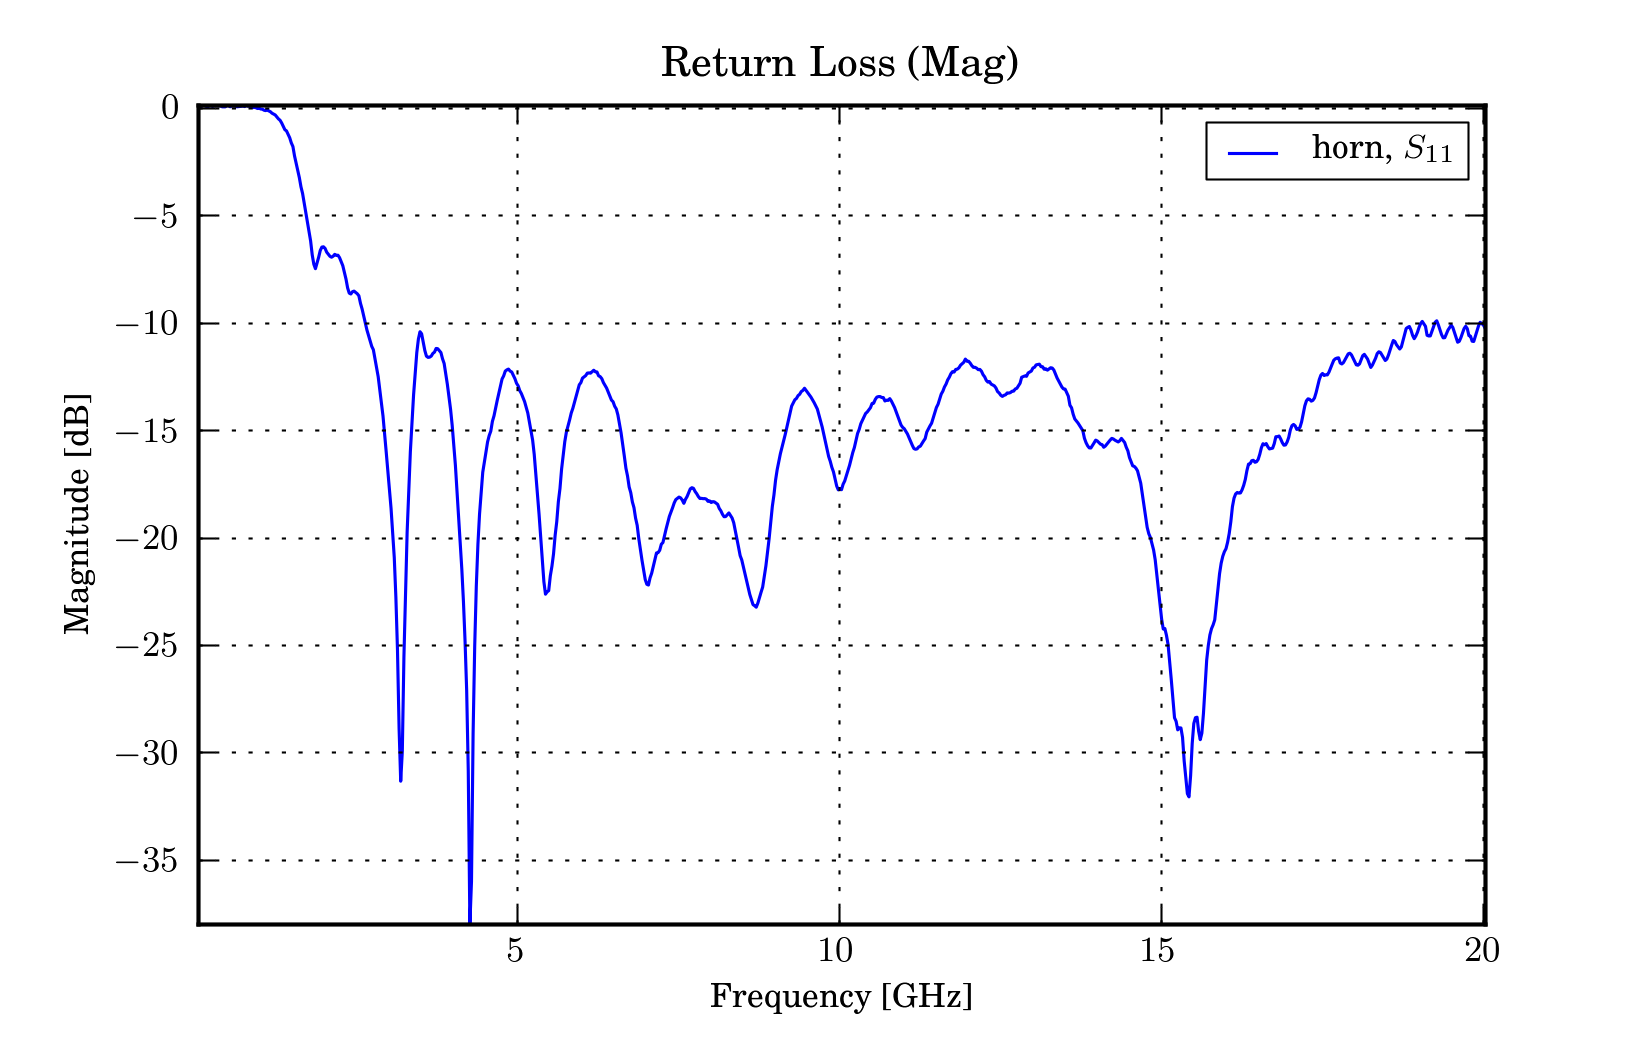
\includegraphics{Return_Loss(Mag).png}
\end{figure}

\begin{Verbatim}[commandchars=\\\{\}]
\PYG{c}{\PYGZsh{} plot phase of S11}
\PYG{n}{pylab}\PYG{o}{.}\PYG{n}{figure}\PYG{p}{(}\PYG{l+m+mi}{2}\PYG{p}{)}
\PYG{n}{pylab}\PYG{o}{.}\PYG{n}{title}\PYG{p}{(}\PYG{l+s}{'}\PYG{l+s}{Return Loss (Phase)}\PYG{l+s}{'}\PYG{p}{)}
\PYG{c}{\PYGZsh{} all keyword arguments are passed to matplotlib.plot command}
\PYG{n}{horn}\PYG{o}{.}\PYG{n}{plot\PYGZus{}s\PYGZus{}deg}\PYG{p}{(}\PYG{l+m+mi}{0}\PYG{p}{,}\PYG{l+m+mi}{0}\PYG{p}{,} \PYG{n}{label}\PYG{o}{=}\PYG{l+s}{'}\PYG{l+s}{Broadband Horn Antenna}\PYG{l+s}{'}\PYG{p}{,} \PYG{n}{color}\PYG{o}{=}\PYG{l+s}{'}\PYG{l+s}{r}\PYG{l+s}{'}\PYG{p}{,} \PYG{n}{linewidth}\PYG{o}{=}\PYG{l+m+mi}{2}\PYG{p}{)}
\end{Verbatim}
\begin{figure}[htbp]
\centering

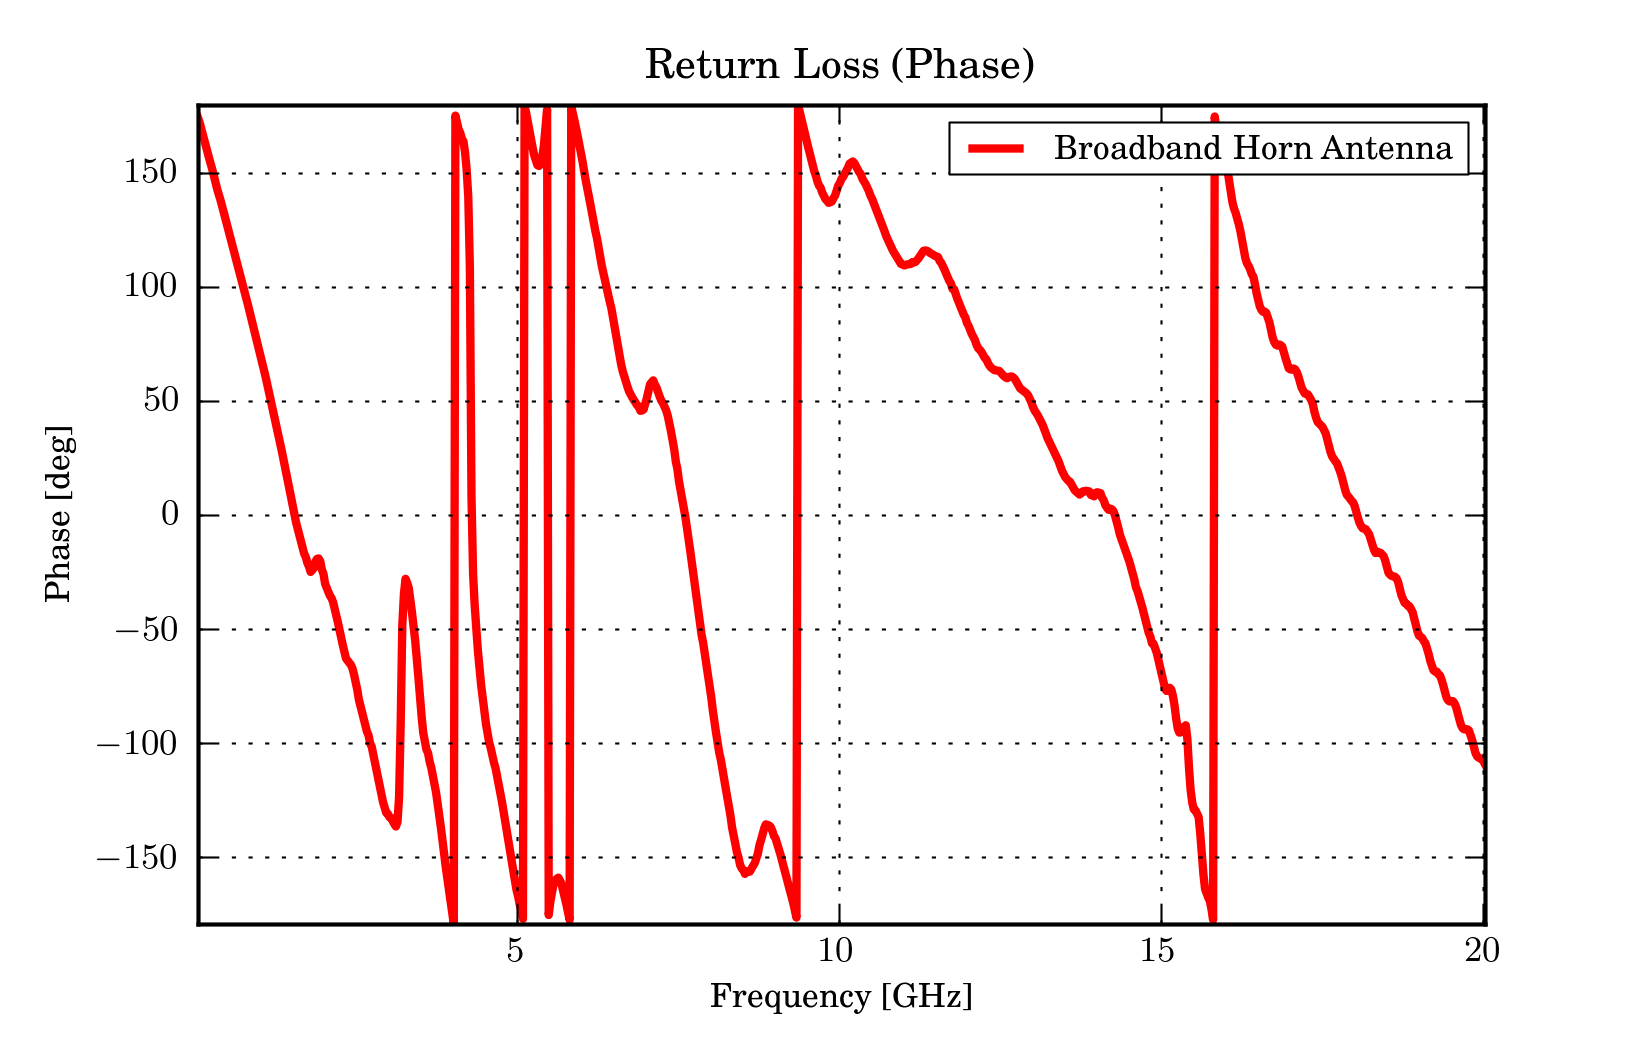
\includegraphics{Return_Loss(Phase).png}
\end{figure}

\begin{Verbatim}[commandchars=\\\{\}]
\PYG{c}{\PYGZsh{} plot unwrapped phase of S11}
\PYG{n}{pylab}\PYG{o}{.}\PYG{n}{figure}\PYG{p}{(}\PYG{l+m+mi}{3}\PYG{p}{)}
\PYG{n}{pylab}\PYG{o}{.}\PYG{n}{title}\PYG{p}{(}\PYG{l+s}{'}\PYG{l+s}{Return Loss (Unwrapped Phase)}\PYG{l+s}{'}\PYG{p}{)}
\PYG{n}{horn}\PYG{o}{.}\PYG{n}{plot\PYGZus{}s\PYGZus{}deg\PYGZus{}unwrapped}\PYG{p}{(}\PYG{l+m+mi}{0}\PYG{p}{,}\PYG{l+m+mi}{0}\PYG{p}{)}
\end{Verbatim}
\begin{figure}[htbp]
\centering

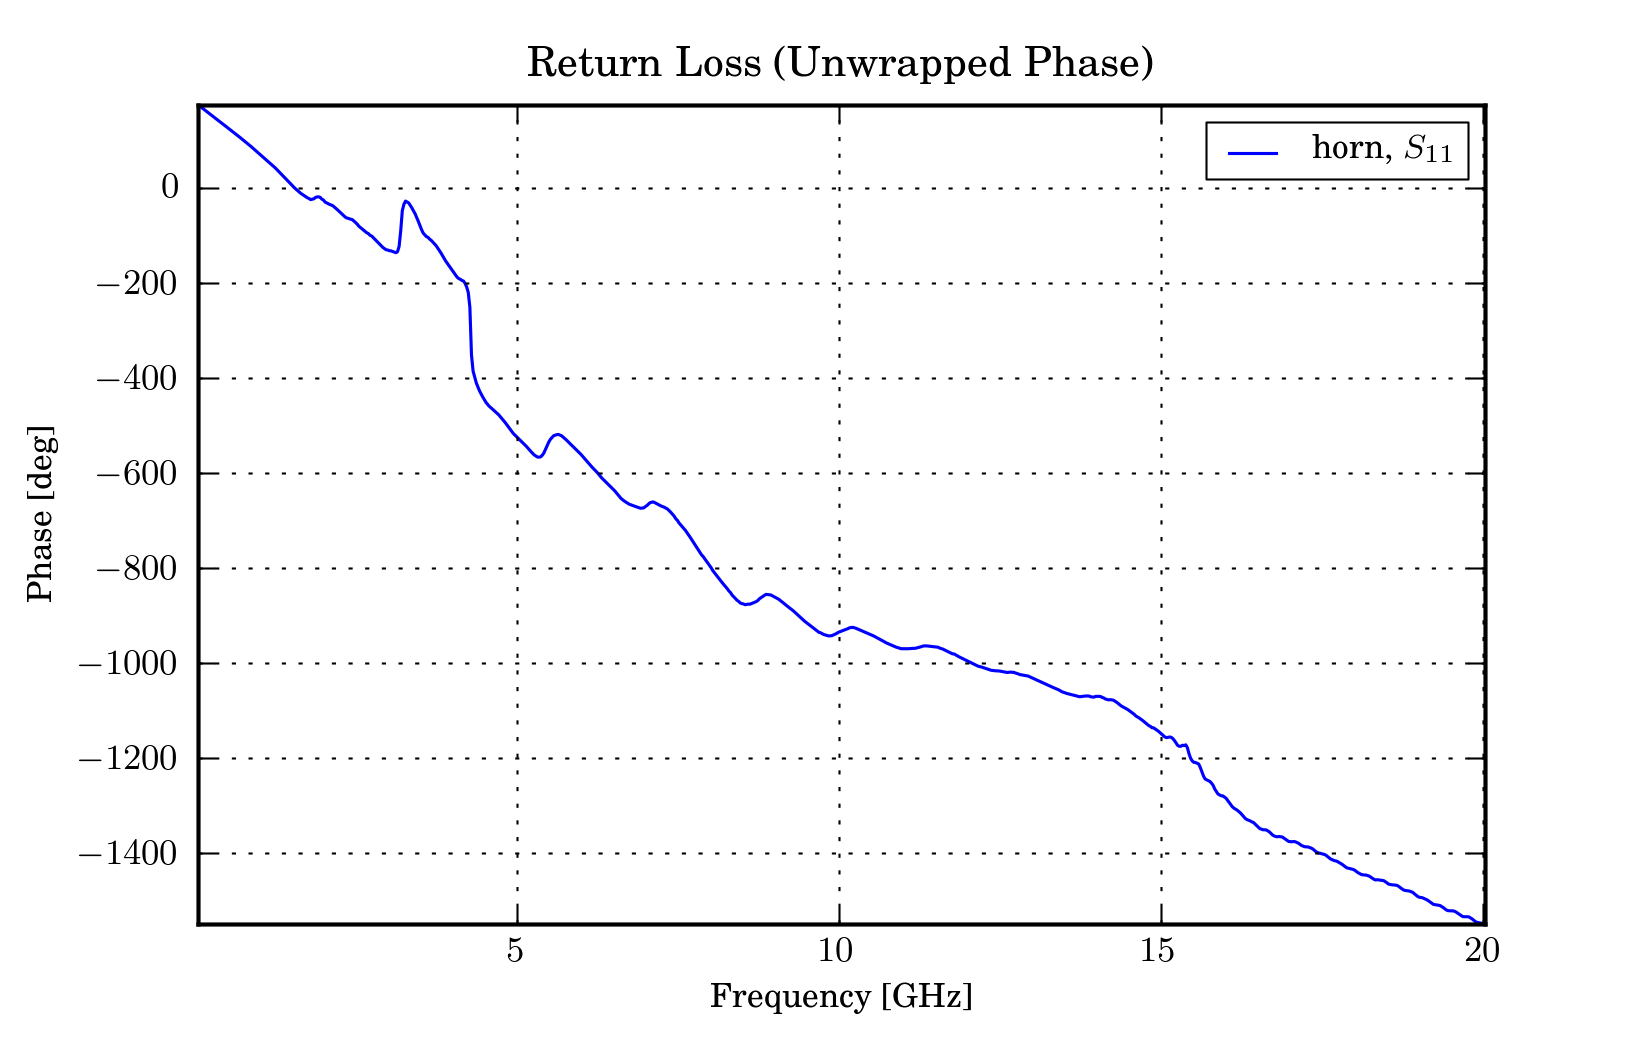
\includegraphics{Return_Loss(Unwrapped_Phase).png}
\end{figure}

\begin{Verbatim}[commandchars=\\\{\}]
\PYG{c}{\PYGZsh{} plot complex S11 on smith chart}
\PYG{n}{pylab}\PYG{o}{.}\PYG{n}{figure}\PYG{p}{(}\PYG{l+m+mi}{5}\PYG{p}{)}
\PYG{n}{horn}\PYG{o}{.}\PYG{n}{plot\PYGZus{}s\PYGZus{}smith}\PYG{p}{(}\PYG{l+m+mi}{0}\PYG{p}{,}\PYG{l+m+mi}{0}\PYG{p}{,} \PYG{n}{show\PYGZus{}legend}\PYG{o}{=}\PYG{n+nb+bp}{False}\PYG{p}{)}
\PYG{n}{pylab}\PYG{o}{.}\PYG{n}{title}\PYG{p}{(}\PYG{l+s}{'}\PYG{l+s}{Return Loss, Smith}\PYG{l+s}{'}\PYG{p}{)}
\end{Verbatim}
\begin{figure}[htbp]
\centering

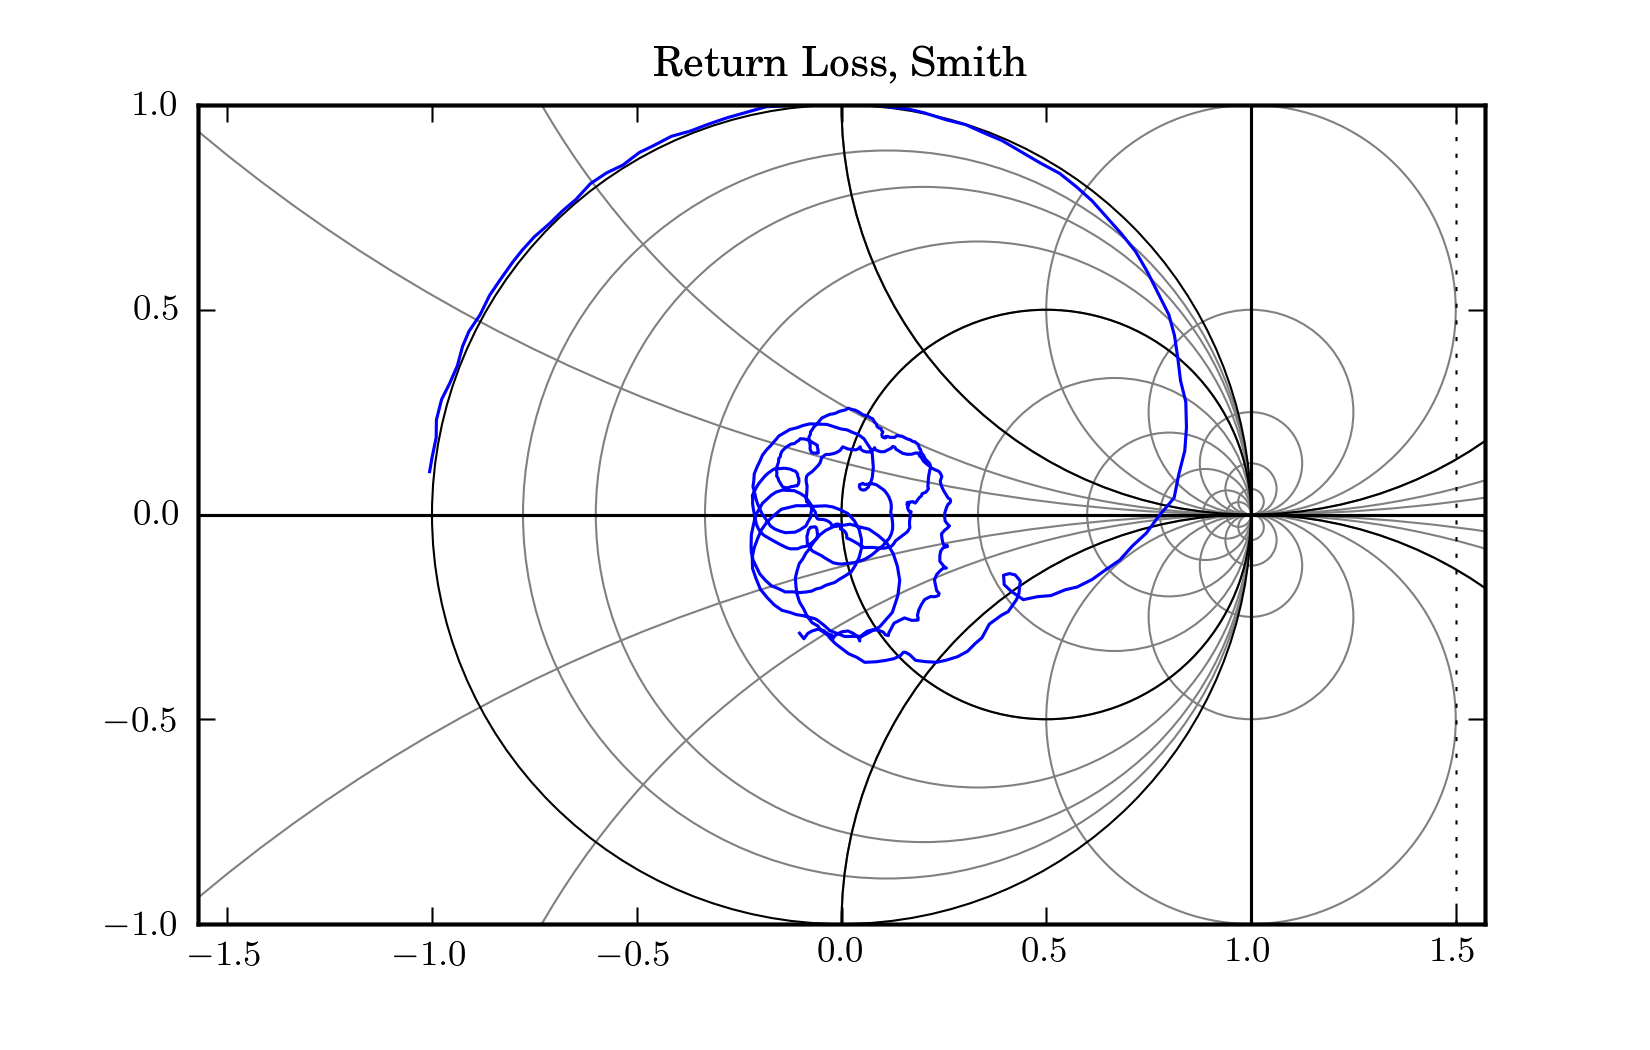
\includegraphics{Return_Loss(Smith).png}
\end{figure}

\begin{Verbatim}[commandchars=\\\{\}]
\PYG{c}{\PYGZsh{} plot complex S11 on polar grid}
\PYG{n}{pylab}\PYG{o}{.}\PYG{n}{figure}\PYG{p}{(}\PYG{l+m+mi}{4}\PYG{p}{)}
\PYG{n}{horn}\PYG{o}{.}\PYG{n}{plot\PYGZus{}s\PYGZus{}polar}\PYG{p}{(}\PYG{l+m+mi}{0}\PYG{p}{,}\PYG{l+m+mi}{0}\PYG{p}{,} \PYG{n}{show\PYGZus{}legend}\PYG{o}{=}\PYG{n+nb+bp}{False}\PYG{p}{)}
\PYG{n}{pylab}\PYG{o}{.}\PYG{n}{title}\PYG{p}{(}\PYG{l+s}{'}\PYG{l+s}{Return Loss, Polar}\PYG{l+s}{'}\PYG{p}{)}
\end{Verbatim}
\begin{figure}[htbp]
\centering

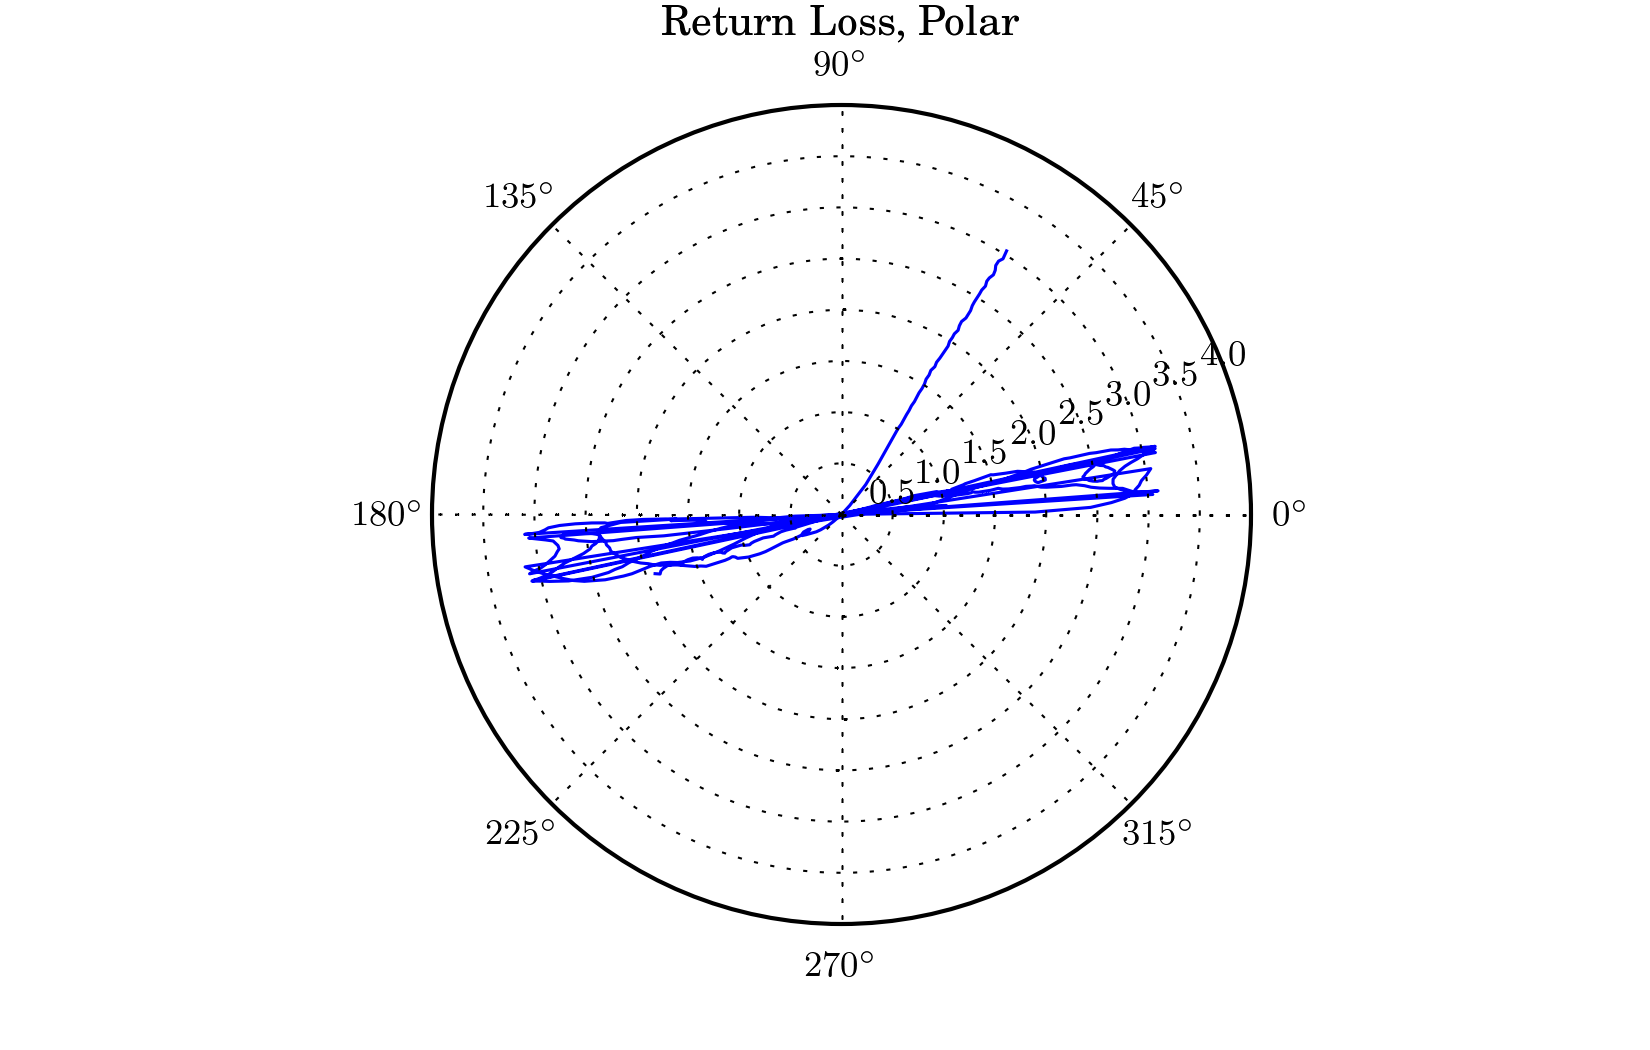
\includegraphics{Return_Loss(Polar).png}
\end{figure}

\begin{Verbatim}[commandchars=\\\{\}]
\PYG{c}{\PYGZsh{}  to save all figures,}
\PYG{n}{mv}\PYG{o}{.}\PYG{n}{save\PYGZus{}all\PYGZus{}figs}\PYG{p}{(}\PYG{l+s}{'}\PYG{l+s}{.}\PYG{l+s}{'}\PYG{p}{,} \PYG{n}{format} \PYG{o}{=} \PYG{p}{[}\PYG{l+s}{'}\PYG{l+s}{png}\PYG{l+s}{'}\PYG{p}{,}\PYG{l+s}{'}\PYG{l+s}{eps}\PYG{l+s}{'}\PYG{p}{]}\PYG{p}{)}
\end{Verbatim}


\section{One-Port Calibration}
\label{examples/oneport_calibration:example-oneport-calibration}\label{examples/oneport_calibration:one-port-calibration}\label{examples/oneport_calibration::doc}

\subsection{Instructive}
\label{examples/oneport_calibration:instructive}
This example is written to be instructive, not concise.:

\begin{Verbatim}[commandchars=\\\{\}]
\PYG{k+kn}{import} \PYG{n+nn}{mwavepy} \PYG{k+kn}{as} \PYG{n+nn}{mv}


\PYG{c}{\PYGZsh{}\PYGZsh{} created necessary data for Calibration class}

\PYG{c}{\PYGZsh{} a list of Network types, holding 'ideal' responses}
\PYG{n}{my\PYGZus{}ideals} \PYG{o}{=} \PYG{p}{[}\PYGZbs{}
        \PYG{n}{mv}\PYG{o}{.}\PYG{n}{Network}\PYG{p}{(}\PYG{l+s}{'}\PYG{l+s}{ideal/short.s1p}\PYG{l+s}{'}\PYG{p}{)}\PYG{p}{,}
        \PYG{n}{mv}\PYG{o}{.}\PYG{n}{Network}\PYG{p}{(}\PYG{l+s}{'}\PYG{l+s}{ideal/open.s1p}\PYG{l+s}{'}\PYG{p}{)}\PYG{p}{,}
        \PYG{n}{mv}\PYG{o}{.}\PYG{n}{Network}\PYG{p}{(}\PYG{l+s}{'}\PYG{l+s}{ideal/load.s1p}\PYG{l+s}{'}\PYG{p}{)}\PYG{p}{,}
        \PYG{p}{]}

\PYG{c}{\PYGZsh{} a list of Network types, holding 'measured' responses}
\PYG{n}{my\PYGZus{}measured} \PYG{o}{=} \PYG{p}{[}\PYGZbs{}
        \PYG{n}{mv}\PYG{o}{.}\PYG{n}{Network}\PYG{p}{(}\PYG{l+s}{'}\PYG{l+s}{measured/short.s1p}\PYG{l+s}{'}\PYG{p}{)}\PYG{p}{,}
        \PYG{n}{mv}\PYG{o}{.}\PYG{n}{Network}\PYG{p}{(}\PYG{l+s}{'}\PYG{l+s}{measured/open.s1p}\PYG{l+s}{'}\PYG{p}{)}\PYG{p}{,}
        \PYG{n}{mv}\PYG{o}{.}\PYG{n}{Network}\PYG{p}{(}\PYG{l+s}{'}\PYG{l+s}{measured/load.s1p}\PYG{l+s}{'}\PYG{p}{)}\PYG{p}{,}
        \PYG{p}{]}

\PYG{c}{\PYGZsh{}\PYGZsh{} create a Calibration instance}
\PYG{n}{cal} \PYG{o}{=} \PYG{n}{mv}\PYG{o}{.}\PYG{n}{Calibration}\PYG{p}{(}\PYGZbs{}
        \PYG{n}{ideals} \PYG{o}{=} \PYG{n}{my\PYGZus{}ideals}\PYG{p}{,}
        \PYG{n}{measured} \PYG{o}{=} \PYG{n}{my\PYGZus{}measured}\PYG{p}{,}
        \PYG{p}{)}


\PYG{c}{\PYGZsh{}\PYGZsh{} run, and apply calibration to a DUT}

\PYG{c}{\PYGZsh{} run calibration algorithm}
\PYG{n}{cal}\PYG{o}{.}\PYG{n}{run}\PYG{p}{(}\PYG{p}{)}

\PYG{c}{\PYGZsh{} apply it to a dut}
\PYG{n}{dut} \PYG{o}{=} \PYG{n}{mv}\PYG{o}{.}\PYG{n}{Network}\PYG{p}{(}\PYG{l+s}{'}\PYG{l+s}{my\PYGZus{}dut.s1p}\PYG{l+s}{'}\PYG{p}{)}
\PYG{n}{dut\PYGZus{}caled} \PYG{o}{=} \PYG{n}{cal}\PYG{o}{.}\PYG{n}{apply\PYGZus{}cal}\PYG{p}{(}\PYG{n}{dut}\PYG{p}{)}

\PYG{c}{\PYGZsh{} plot results}
\PYG{n}{dut\PYGZus{}caled}\PYG{o}{.}\PYG{n}{plot\PYGZus{}s\PYGZus{}db}\PYG{p}{(}\PYG{p}{)}
\PYG{c}{\PYGZsh{} save results}
\PYG{n}{dut\PYGZus{}caled}\PYG{o}{.}\PYG{n}{write\PYGZus{}touchstone}\PYG{p}{(}\PYG{p}{)}
\end{Verbatim}


\subsection{Concise}
\label{examples/oneport_calibration:concise}
This example is meant to be the same as the first except more concise:

\begin{Verbatim}[commandchars=\\\{\}]
\PYG{k+kn}{import} \PYG{n+nn}{mwavepy} \PYG{k+kn}{as} \PYG{n+nn}{mv}

\PYG{n}{my\PYGZus{}ideals} \PYG{o}{=} \PYG{n}{mv}\PYG{o}{.}\PYG{n}{load\PYGZus{}all\PYGZus{}touchstones\PYGZus{}in\PYGZus{}dir}\PYG{p}{(}\PYG{l+s}{'}\PYG{l+s}{ideals/}\PYG{l+s}{'}\PYG{p}{)}
\PYG{n}{my\PYGZus{}measured} \PYG{o}{=} \PYG{n}{mv}\PYG{o}{.}\PYG{n}{load\PYGZus{}all\PYGZus{}touchstones\PYGZus{}in\PYGZus{}dir}\PYG{p}{(}\PYG{l+s}{'}\PYG{l+s}{measured/}\PYG{l+s}{'}\PYG{p}{)}


\PYG{c}{\PYGZsh{}\PYGZsh{} create a Calibration instance}
\PYG{n}{cal} \PYG{o}{=} \PYG{n}{mv}\PYG{o}{.}\PYG{n}{Calibration}\PYG{p}{(}\PYGZbs{}
        \PYG{n}{ideals} \PYG{o}{=} \PYG{p}{[}\PYG{n}{my\PYGZus{}ideals}\PYG{p}{[}\PYG{n}{k}\PYG{p}{]} \PYG{k}{for} \PYG{n}{k} \PYG{o+ow}{in} \PYG{p}{[}\PYG{l+s}{'}\PYG{l+s}{short}\PYG{l+s}{'}\PYG{p}{,}\PYG{l+s}{'}\PYG{l+s}{open}\PYG{l+s}{'}\PYG{p}{,}\PYG{l+s}{'}\PYG{l+s}{load}\PYG{l+s}{'}\PYG{p}{]}\PYG{p}{]}\PYG{p}{,}
        \PYG{n}{measured} \PYG{o}{=} \PYG{p}{[}\PYG{n}{my\PYGZus{}measured}\PYG{p}{[}\PYG{n}{k}\PYG{p}{]} \PYG{k}{for} \PYG{n}{k} \PYG{o+ow}{in} \PYG{p}{[}\PYG{l+s}{'}\PYG{l+s}{short}\PYG{l+s}{'}\PYG{p}{,}\PYG{l+s}{'}\PYG{l+s}{open}\PYG{l+s}{'}\PYG{p}{,}\PYG{l+s}{'}\PYG{l+s}{load}\PYG{l+s}{'}\PYG{p}{]}\PYG{p}{]}\PYG{p}{,}
        \PYG{p}{)}

\PYG{c}{\PYGZsh{}\PYGZsh{} what you do with 'cal' may  may be similar to above example}
\end{Verbatim}


\section{Two-Port Calibration}
\label{examples/twoport_calibration::doc}\label{examples/twoport_calibration:two-port-calibration}
This is an example of how to setup two-port calibration. For more detailed explaination see \code{calibration}:

\begin{Verbatim}[commandchars=\\\{\}]
\PYG{k+kn}{import} \PYG{n+nn}{mwavepy} \PYG{k+kn}{as} \PYG{n+nn}{mv}


\PYG{c}{\PYGZsh{}\PYGZsh{} created necessary data for Calibration class}

\PYG{c}{\PYGZsh{} a list of Network types, holding 'ideal' responses}
\PYG{n}{my\PYGZus{}ideals} \PYG{o}{=} \PYG{p}{[}\PYGZbs{}
        \PYG{n}{mv}\PYG{o}{.}\PYG{n}{Network}\PYG{p}{(}\PYG{l+s}{'}\PYG{l+s}{ideal/thru.s2p}\PYG{l+s}{'}\PYG{p}{)}\PYG{p}{,}
        \PYG{n}{mv}\PYG{o}{.}\PYG{n}{Network}\PYG{p}{(}\PYG{l+s}{'}\PYG{l+s}{ideal/line.s2p}\PYG{l+s}{'}\PYG{p}{)}\PYG{p}{,}
        \PYG{n}{mv}\PYG{o}{.}\PYG{n}{Network}\PYG{p}{(}\PYG{l+s}{'}\PYG{l+s}{ideal/short, short.s2p}\PYG{l+s}{'}\PYG{p}{)}\PYG{p}{,}
        \PYG{p}{]}

\PYG{c}{\PYGZsh{} a list of Network types, holding 'measured' responses}
\PYG{n}{my\PYGZus{}measured} \PYG{o}{=} \PYG{p}{[}\PYGZbs{}
        \PYG{n}{mv}\PYG{o}{.}\PYG{n}{Network}\PYG{p}{(}\PYG{l+s}{'}\PYG{l+s}{measured/thru.s2p}\PYG{l+s}{'}\PYG{p}{)}\PYG{p}{,}
        \PYG{n}{mv}\PYG{o}{.}\PYG{n}{Network}\PYG{p}{(}\PYG{l+s}{'}\PYG{l+s}{measured/line.s2p}\PYG{l+s}{'}\PYG{p}{)}\PYG{p}{,}
        \PYG{n}{mv}\PYG{o}{.}\PYG{n}{Network}\PYG{p}{(}\PYG{l+s}{'}\PYG{l+s}{measured/short, short.s2p}\PYG{l+s}{'}\PYG{p}{)}\PYG{p}{,}
        \PYG{p}{]}


\PYG{c}{\PYGZsh{}\PYGZsh{} create a Calibration instance}
\PYG{n}{cal} \PYG{o}{=} \PYG{n}{mv}\PYG{o}{.}\PYG{n}{Calibration}\PYG{p}{(}\PYGZbs{}
        \PYG{n}{ideals} \PYG{o}{=} \PYG{n}{my\PYGZus{}ideals}\PYG{p}{,}
        \PYG{n}{measured} \PYG{o}{=} \PYG{n}{my\PYGZus{}measured}\PYG{p}{,}
        \PYG{p}{)}


\PYG{c}{\PYGZsh{}\PYGZsh{} run, and apply calibration to a DUT}

\PYG{c}{\PYGZsh{} run calibration algorithm}
\PYG{n}{cal}\PYG{o}{.}\PYG{n}{run}\PYG{p}{(}\PYG{p}{)}

\PYG{c}{\PYGZsh{} apply it to a dut}
\PYG{n}{dut} \PYG{o}{=} \PYG{n}{mv}\PYG{o}{.}\PYG{n}{Network}\PYG{p}{(}\PYG{l+s}{'}\PYG{l+s}{my\PYGZus{}dut.s2p}\PYG{l+s}{'}\PYG{p}{)}
\PYG{n}{dut\PYGZus{}caled} \PYG{o}{=} \PYG{n}{cal}\PYG{o}{.}\PYG{n}{apply\PYGZus{}cal}\PYG{p}{(}\PYG{n}{dut}\PYG{p}{)}

\PYG{c}{\PYGZsh{} plot results}
\PYG{n}{dut\PYGZus{}caled}\PYG{o}{.}\PYG{n}{plot\PYGZus{}s\PYGZus{}db}\PYG{p}{(}\PYG{p}{)}
\PYG{c}{\PYGZsh{} save results}
\PYG{n}{dut\PYGZus{}caled}\PYG{o}{.}\PYG{n}{write\PYGZus{}touchstone}\PYG{p}{(}\PYG{p}{)}
\end{Verbatim}


\section{VNA Noise Analysis}
\label{examples/vna_noise_analysis:vna-noise-analysis}\label{examples/vna_noise_analysis:example-vna-noise-analysis}\label{examples/vna_noise_analysis::doc}
This example records a series of sweeps from a vna to touchstone files, named in a chronological order. These are then used to characterize the noise of a vna


\subsection{Touchstone File Retrieval}
\label{examples/vna_noise_analysis:touchstone-file-retrieval}
\begin{Verbatim}[commandchars=\\\{\}]
\PYG{k+kn}{import} \PYG{n+nn}{mwavepy} \PYG{k+kn}{as} \PYG{n+nn}{mv}
\PYG{k+kn}{import} \PYG{n+nn}{os}\PYG{o}{,}\PYG{n+nn}{datetime}

\PYG{n}{nsweeps} \PYG{o}{=} \PYG{l+m+mi}{101} \PYG{c}{\PYGZsh{} number of sweeps to take}
\PYG{n+nb}{dir} \PYG{o}{=} \PYG{n}{datetime}\PYG{o}{.}\PYG{n}{datetime}\PYG{o}{.}\PYG{n}{now}\PYG{p}{(}\PYG{p}{)}\PYG{o}{.}\PYG{n}{date}\PYG{p}{(}\PYG{p}{)}\PYG{o}{.}\PYG{n}{\PYGZus{}\PYGZus{}str\PYGZus{}\PYGZus{}}\PYG{p}{(}\PYG{p}{)} \PYG{c}{\PYGZsh{} directory to save files in}

\PYG{n}{myvna} \PYG{o}{=} \PYG{n}{mv}\PYG{o}{.}\PYG{n}{vna}\PYG{o}{.}\PYG{n}{HP8720}\PYG{p}{(}\PYG{p}{)} \PYG{c}{\PYGZsh{} HP8510 also available}
\PYG{n}{os}\PYG{o}{.}\PYG{n}{mkdir}\PYG{p}{(}\PYG{n+nb}{dir}\PYG{p}{)}
\PYG{k}{for} \PYG{n}{k} \PYG{o+ow}{in} \PYG{n+nb}{range}\PYG{p}{(}\PYG{n}{nsweeps}\PYG{p}{)}\PYG{p}{:}
        \PYG{k}{print}  \PYG{n}{k}
        \PYG{n}{ntwk} \PYG{o}{=} \PYG{n}{myvna}\PYG{o}{.}\PYG{n}{s11}
        \PYG{n}{date\PYGZus{}string} \PYG{o}{=} \PYG{n}{datetime}\PYG{o}{.}\PYG{n}{datetime}\PYG{o}{.}\PYG{n}{now}\PYG{p}{(}\PYG{p}{)}\PYG{o}{.}\PYG{n}{\PYGZus{}\PYGZus{}str\PYGZus{}\PYGZus{}}\PYG{p}{(}\PYG{p}{)}\PYG{o}{.}\PYG{n}{replace}\PYG{p}{(}\PYG{l+s}{'}\PYG{l+s}{:}\PYG{l+s}{'}\PYG{p}{,}\PYG{l+s}{'}\PYG{l+s}{-}\PYG{l+s}{'}\PYG{p}{)}
        \PYG{n}{ntwk}\PYG{o}{.}\PYG{n}{write\PYGZus{}touchstone}\PYG{p}{(}\PYG{n+nb}{dir} \PYG{o}{+}\PYG{l+s}{'}\PYG{l+s}{/}\PYG{l+s}{'}\PYG{o}{+} \PYG{n}{date\PYGZus{}string}\PYG{p}{)}

\PYG{n}{myvna}\PYG{o}{.}\PYG{n}{close}\PYG{p}{(}\PYG{p}{)}
\end{Verbatim}


\subsection{Noise Analysis}
\label{examples/vna_noise_analysis:noise-analysis}
Calculates and plots various metrics of noise, given a directory of
touchstones files, as would be created from the previous script

\begin{Verbatim}[commandchars=\\\{\}]
\PYG{k+kn}{import} \PYG{n+nn}{mwavepy} \PYG{k+kn}{as} \PYG{n+nn}{mv}
\PYG{k+kn}{from} \PYG{n+nn}{pylab} \PYG{k+kn}{import} \PYG{o}{*}

\PYG{n+nb}{dir} \PYG{o}{=} \PYG{l+s}{'}\PYG{l+s}{2010-12-03}\PYG{l+s}{'} \PYG{c}{\PYGZsh{} directory of touchstone files}
\PYG{n}{npoints} \PYG{o}{=} \PYG{l+m+mi}{3} \PYG{c}{\PYGZsh{} number of frequency points to calculate statistics for}


\PYG{c}{\PYGZsh{} load all touchstones in directory into a dictionary, and sort keys}
\PYG{n}{data} \PYG{o}{=} \PYG{n}{mv}\PYG{o}{.}\PYG{n}{load\PYGZus{}all\PYGZus{}touchstones}\PYG{p}{(}\PYG{n+nb}{dir}\PYG{o}{+}\PYG{l+s}{'}\PYG{l+s}{/}\PYG{l+s}{'}\PYG{p}{)}
\PYG{n}{keys}\PYG{o}{=}\PYG{n}{data}\PYG{o}{.}\PYG{n}{keys}\PYG{p}{(}\PYG{p}{)}
\PYG{n}{keys}\PYG{o}{.}\PYG{n}{sort}\PYG{p}{(}\PYG{p}{)}

\PYG{c}{\PYGZsh{} length of frequency vector of each network}
\PYG{n}{f\PYGZus{}len} \PYG{o}{=} \PYG{n}{data}\PYG{p}{[}\PYG{n}{keys}\PYG{p}{[}\PYG{l+m+mi}{0}\PYG{p}{]}\PYG{p}{]}\PYG{o}{.}\PYG{n}{frequency}\PYG{o}{.}\PYG{n}{npoints}
\PYG{c}{\PYGZsh{} frequency vector indecies at which we will calculate the statistics}
\PYG{n}{f\PYGZus{}vector} \PYG{o}{=} \PYG{p}{[}\PYG{n+nb}{int}\PYG{p}{(}\PYG{n}{k}\PYG{p}{)} \PYG{k}{for} \PYG{n}{k} \PYG{o+ow}{in} \PYG{n}{linspace}\PYG{p}{(}\PYG{l+m+mi}{0}\PYG{p}{,}\PYG{n}{f\PYGZus{}len}\PYG{o}{-}\PYG{l+m+mi}{1}\PYG{p}{,} \PYG{n}{npoints}\PYG{p}{)}\PYG{p}{]}

\PYG{c}{\PYGZsh{}loop through the frequencies of interest and calculate statistics}
\PYG{k}{for} \PYG{n}{f} \PYG{o+ow}{in} \PYG{n}{f\PYGZus{}vector}\PYG{p}{:}
        \PYG{c}{\PYGZsh{} for legends}
        \PYG{n}{f\PYGZus{}scaled} \PYG{o}{=} \PYG{n}{data}\PYG{p}{[}\PYG{n}{keys}\PYG{p}{[}\PYG{l+m+mi}{0}\PYG{p}{]}\PYG{p}{]}\PYG{o}{.}\PYG{n}{frequency}\PYG{o}{.}\PYG{n}{f\PYGZus{}scaled}\PYG{p}{[}\PYG{n}{f}\PYG{p}{]}
        \PYG{n}{f\PYGZus{}unit} \PYG{o}{=} \PYG{n}{data}\PYG{p}{[}\PYG{n}{keys}\PYG{p}{[}\PYG{l+m+mi}{0}\PYG{p}{]}\PYG{p}{]}\PYG{o}{.}\PYG{n}{frequency}\PYG{o}{.}\PYG{n}{unit}

        \PYG{c}{\PYGZsh{} z is 1d complex array of the s11 at the current frequency, it is}
        \PYG{c}{\PYGZsh{} as long as the number of touchsone files}
        \PYG{n}{z} \PYG{o}{=} \PYG{n}{array}\PYG{p}{(} \PYG{p}{[}\PYG{p}{(}\PYG{n}{data}\PYG{p}{[}\PYG{n}{keys}\PYG{p}{[}\PYG{n}{k}\PYG{p}{]}\PYG{p}{]}\PYG{p}{)}\PYG{o}{.}\PYG{n}{s}\PYG{p}{[}\PYG{n}{f}\PYG{p}{,}\PYG{l+m+mi}{0}\PYG{p}{,}\PYG{l+m+mi}{0}\PYG{p}{]} \PYG{k}{for} \PYG{n}{k} \PYG{o+ow}{in} \PYG{n+nb}{range}\PYG{p}{(}\PYG{n+nb}{len}\PYG{p}{(}\PYG{n}{keys}\PYG{p}{)}\PYG{p}{)}\PYG{p}{]}\PYG{p}{)}
        \PYG{n}{phase\PYGZus{}change} \PYG{o}{=} \PYG{n}{mv}\PYG{o}{.}\PYG{n}{complex\PYGZus{}2\PYGZus{}degree}\PYG{p}{(}\PYG{n}{z} \PYG{o}{*} \PYG{l+m+mi}{1}\PYG{o}{/}\PYG{n}{z}\PYG{p}{[}\PYG{l+m+mi}{0}\PYG{p}{]}\PYG{p}{)}
        \PYG{n}{phase\PYGZus{}change} \PYG{o}{=} \PYG{n}{phase\PYGZus{}change} \PYG{o}{-} \PYG{n}{mean}\PYG{p}{(}\PYG{n}{phase\PYGZus{}change}\PYG{p}{)}
        \PYG{n}{mag\PYGZus{}change} \PYG{o}{=} \PYG{n}{mv}\PYG{o}{.}\PYG{n}{complex\PYGZus{}2\PYGZus{}magnitude}\PYG{p}{(}\PYG{n}{z}\PYG{o}{-}\PYG{n}{z}\PYG{p}{[}\PYG{l+m+mi}{0}\PYG{p}{]}\PYG{p}{)}

        \PYG{n}{figure}\PYG{p}{(}\PYG{l+m+mi}{1}\PYG{p}{)}
        \PYG{n}{title}\PYG{p}{(}\PYG{l+s}{'}\PYG{l+s}{Complex Drift}\PYG{l+s}{'}\PYG{p}{)}
        \PYG{n}{plot}\PYG{p}{(}\PYG{n}{z}\PYG{o}{.}\PYG{n}{real}\PYG{p}{,}\PYG{n}{z}\PYG{o}{.}\PYG{n}{imag}\PYG{p}{,}\PYG{l+s}{'}\PYG{l+s}{.}\PYG{l+s}{'}\PYG{p}{,}\PYG{n}{label}\PYG{o}{=}\PYG{l+s}{'}\PYG{l+s}{f = }\PYG{l+s+si}{\PYGZpc{}i}\PYG{l+s+si}{\PYGZpc{}s}\PYG{l+s}{'}\PYG{o}{\PYGZpc{}} \PYG{p}{(} \PYG{n}{f\PYGZus{}scaled}\PYG{p}{,}\PYG{n}{f\PYGZus{}unit}\PYG{p}{)}\PYG{p}{)}
        \PYG{n}{axis}\PYG{p}{(}\PYG{l+s}{'}\PYG{l+s}{equal}\PYG{l+s}{'}\PYG{p}{)}
        \PYG{n}{legend}\PYG{p}{(}\PYG{p}{)}
        \PYG{n}{mv}\PYG{o}{.}\PYG{n}{smith}\PYG{p}{(}\PYG{p}{)}

        \PYG{n}{figure}\PYG{p}{(}\PYG{l+m+mi}{2}\PYG{p}{)}
        \PYG{n}{title}\PYG{p}{(}\PYG{l+s}{'}\PYG{l+s}{Phase Drift vs. Time}\PYG{l+s}{'}\PYG{p}{)}
        \PYG{n}{xlabel}\PYG{p}{(}\PYG{l+s}{'}\PYG{l+s}{Sample [n]}\PYG{l+s}{'}\PYG{p}{)}
        \PYG{n}{ylabel}\PYG{p}{(}\PYG{l+s}{'}\PYG{l+s}{Phase From Mean [deg]}\PYG{l+s}{'}\PYG{p}{)}
        \PYG{n}{plot}\PYG{p}{(}\PYG{n}{phase\PYGZus{}change}\PYG{p}{,}\PYG{n}{label}\PYG{o}{=}\PYG{l+s}{'}\PYG{l+s}{f = }\PYG{l+s+si}{\PYGZpc{}i}\PYG{l+s+si}{\PYGZpc{}s}\PYG{l+s}{, \PYGZdl{}}\PYG{l+s}{\PYGZbs{}}\PYG{l+s}{sigma=}\PYG{l+s+si}{\PYGZpc{}.1f}\PYG{l+s}{\PYGZdl{}}\PYG{l+s}{'}\PYG{o}{\PYGZpc{}}\PYG{p}{(}\PYG{n}{f\PYGZus{}scaled}\PYG{p}{,}\PYG{n}{f\PYGZus{}unit}\PYG{p}{,}\PYG{n}{std}\PYG{p}{(}\PYG{n}{phase\PYGZus{}change}\PYG{p}{)}\PYG{p}{)}\PYG{p}{)}
        \PYG{n}{legend}\PYG{p}{(}\PYG{p}{)}

        \PYG{n}{figure}\PYG{p}{(}\PYG{l+m+mi}{3}\PYG{p}{)}
        \PYG{n}{title}\PYG{p}{(}\PYG{l+s}{'}\PYG{l+s}{Phase Drift Distrobution}\PYG{l+s}{'}\PYG{p}{)}
        \PYG{n}{xlabel}\PYG{p}{(}\PYG{l+s}{'}\PYG{l+s}{Phase From Mean[deg]}\PYG{l+s}{'}\PYG{p}{)}
        \PYG{n}{ylabel}\PYG{p}{(}\PYG{l+s}{'}\PYG{l+s}{Frequency Of Occurrence}\PYG{l+s}{'}\PYG{p}{)}
        \PYG{n}{hist}\PYG{p}{(}\PYG{n}{phase\PYGZus{}change}\PYG{p}{,}\PYG{n}{alpha}\PYG{o}{=}\PYG{o}{.}\PYG{l+m+mi}{5}\PYG{p}{,}\PYG{n}{bins}\PYG{o}{=}\PYG{l+m+mi}{21}\PYG{p}{,}\PYG{n}{histtype}\PYG{o}{=}\PYG{l+s}{'}\PYG{l+s}{stepfilled}\PYG{l+s}{'}\PYG{p}{,}\PYGZbs{}
                \PYG{n}{label}\PYG{o}{=}\PYG{l+s}{'}\PYG{l+s}{f = }\PYG{l+s+si}{\PYGZpc{}i}\PYG{l+s+si}{\PYGZpc{}s}\PYG{l+s}{, \PYGZdl{}}\PYG{l+s}{\PYGZbs{}}\PYG{l+s}{sigma=}\PYG{l+s+si}{\PYGZpc{}.1f}\PYG{l+s}{\PYGZdl{}}\PYG{l+s}{'}\PYG{o}{\PYGZpc{}}\PYG{p}{(}\PYG{n}{f\PYGZus{}scaled}\PYG{p}{,}\PYG{n}{f\PYGZus{}unit}\PYG{p}{,}\PYG{n}{std}\PYG{p}{(}\PYG{n}{phase\PYGZus{}change}\PYG{p}{)}\PYG{p}{)} \PYG{p}{)}
        \PYG{n}{legend}\PYG{p}{(}\PYG{p}{)}
        \PYG{n}{figure}\PYG{p}{(}\PYG{l+m+mi}{4}\PYG{p}{)}
        \PYG{n}{title}\PYG{p}{(}\PYG{l+s}{'}\PYG{l+s}{FFT of Phase Drift}\PYG{l+s}{'}\PYG{p}{)}
        \PYG{n}{ylabel}\PYG{p}{(}\PYG{l+s}{'}\PYG{l+s}{Power [dB]}\PYG{l+s}{'}\PYG{p}{)}
        \PYG{n}{xlabel}\PYG{p}{(}\PYG{l+s}{'}\PYG{l+s}{Sample Frequency [?]}\PYG{l+s}{'}\PYG{p}{)}
        \PYG{n}{plot}\PYG{p}{(}\PYG{n}{log10}\PYG{p}{(}\PYG{n+nb}{abs}\PYG{p}{(}\PYG{n}{fftshift}\PYG{p}{(}\PYG{n}{fft}\PYG{p}{(}\PYG{n}{phase\PYGZus{}change}\PYG{p}{)}\PYG{p}{)}\PYG{p}{)}\PYG{p}{)}\PYG{p}{[}\PYG{n+nb}{len}\PYG{p}{(}\PYG{n}{keys}\PYG{p}{)}\PYG{o}{/}\PYG{l+m+mi}{2}\PYG{o}{+}\PYG{l+m+mi}{1}\PYG{p}{:}\PYG{p}{]}\PYG{p}{)}

\PYG{n}{draw}\PYG{p}{(}\PYG{p}{)}\PYG{p}{;}\PYG{n}{show}\PYG{p}{(}\PYG{p}{)}\PYG{p}{;}
\end{Verbatim}
\begin{figure}[htbp]
\centering

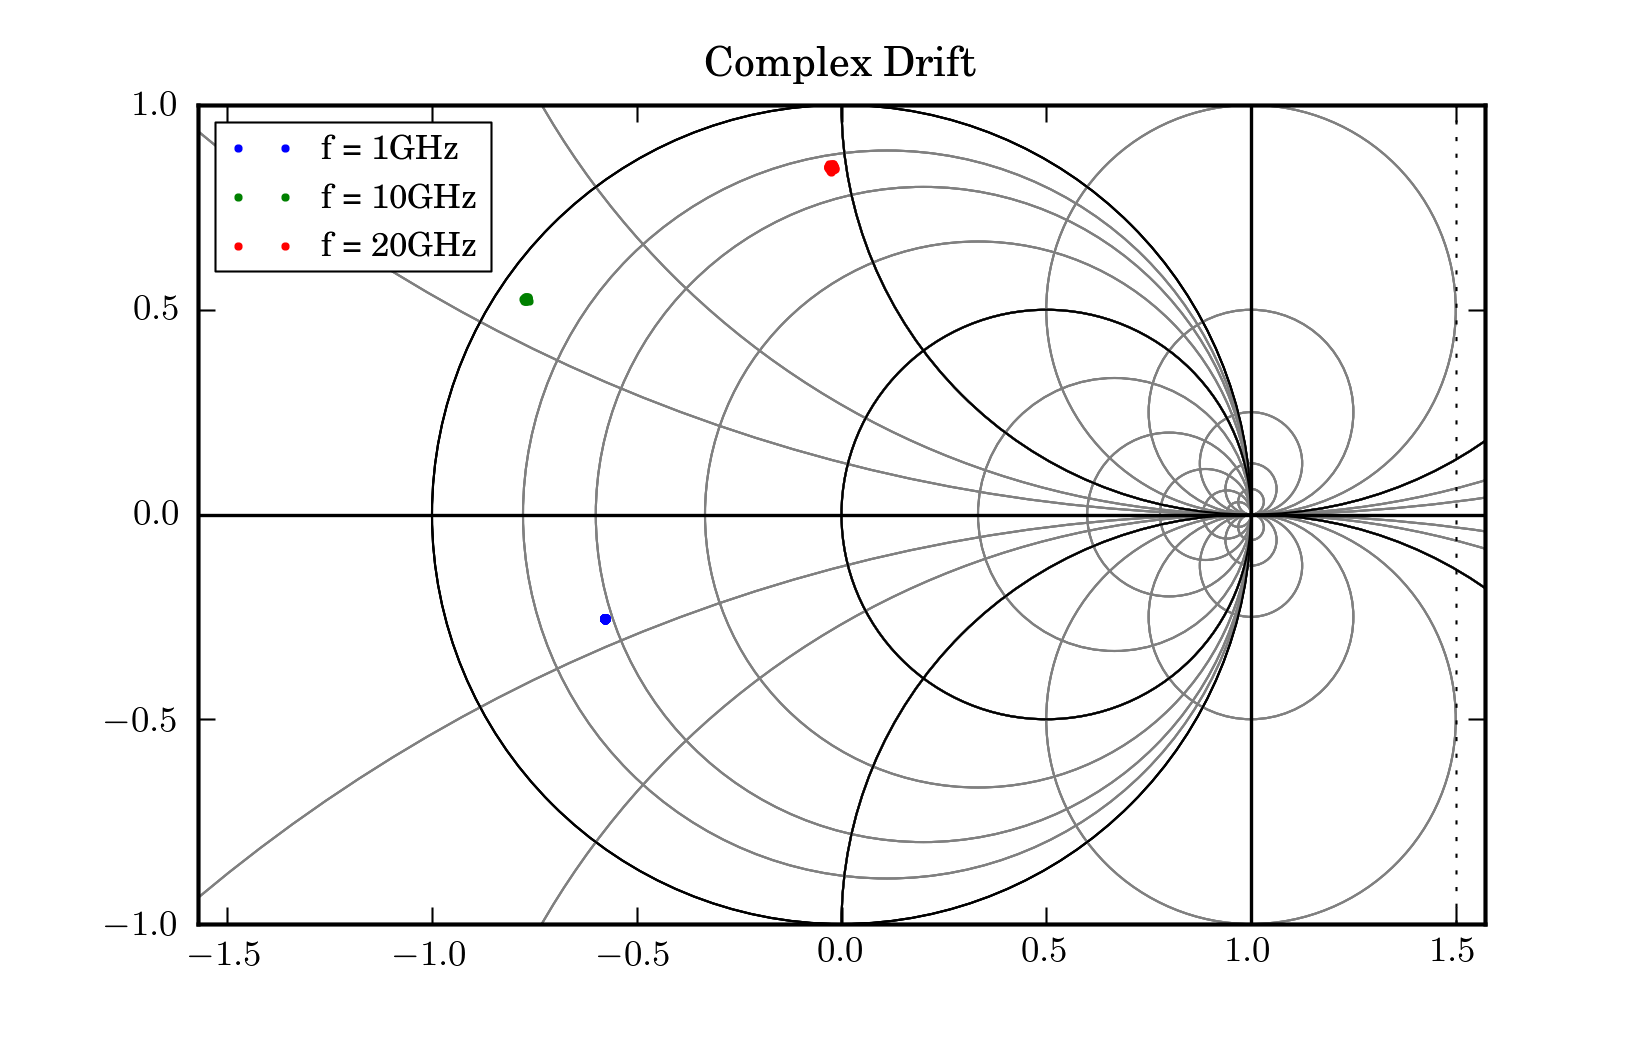
\includegraphics{ComplexDrift.png}
\end{figure}
\begin{figure}[htbp]
\centering

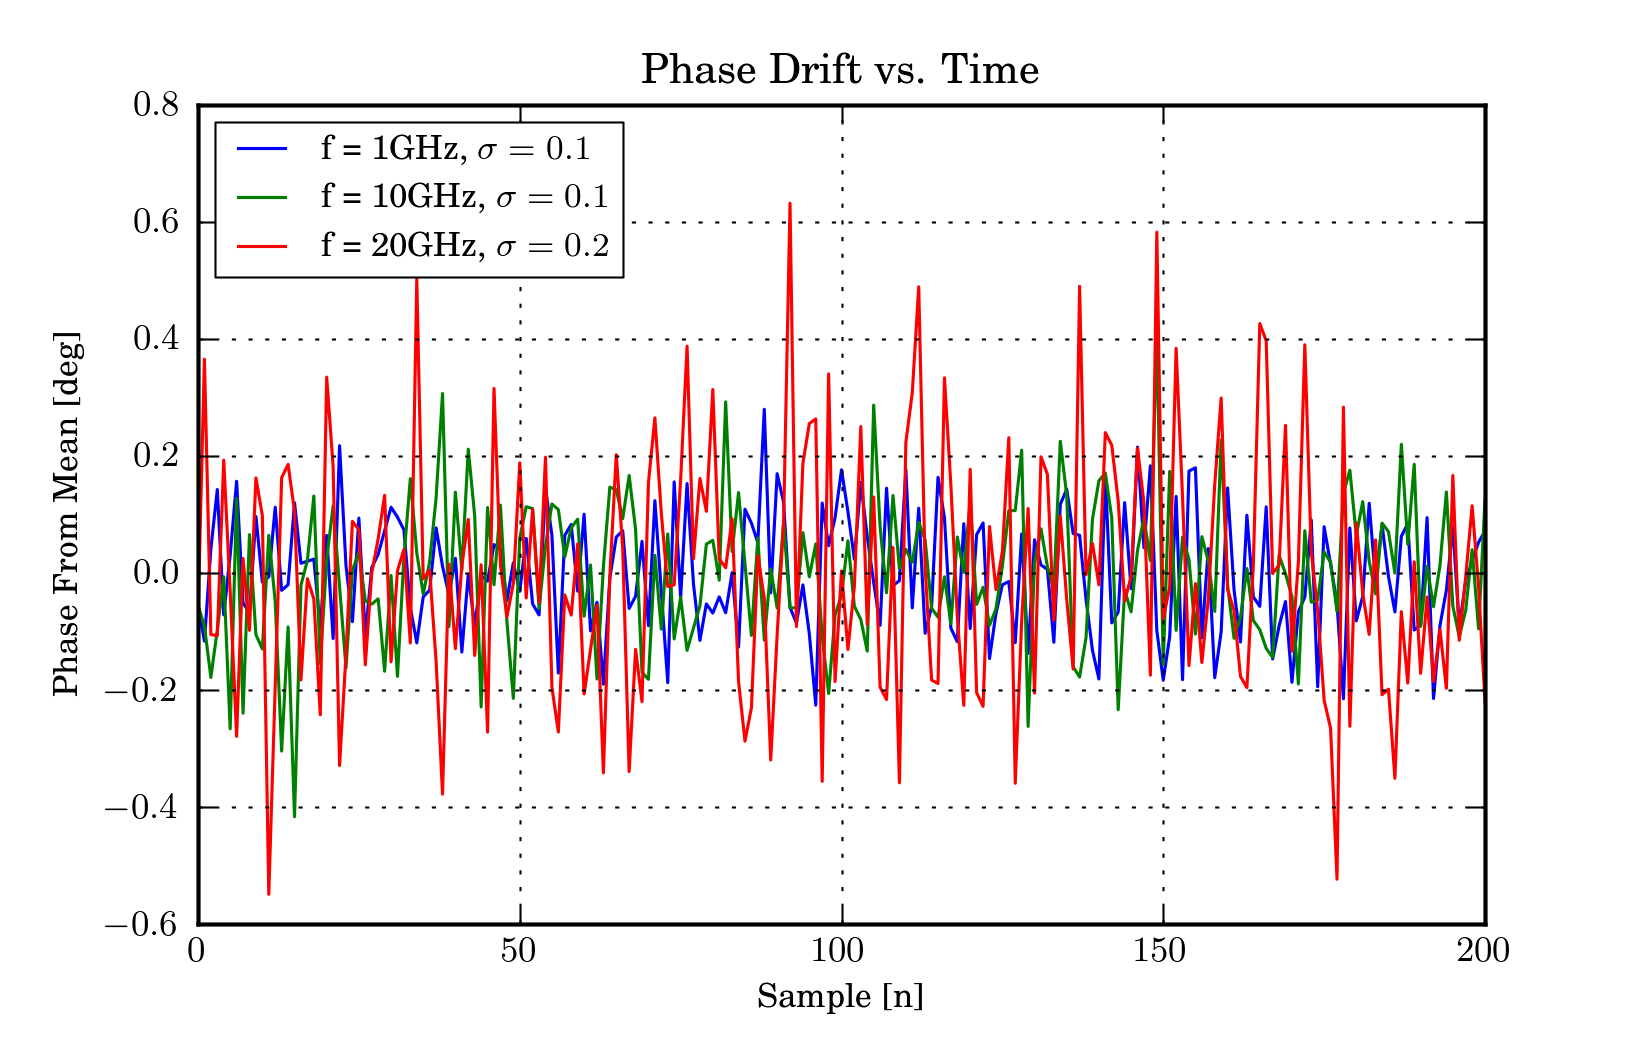
\includegraphics{PhaseDriftvsTime.png}
\end{figure}
\begin{figure}[htbp]
\centering

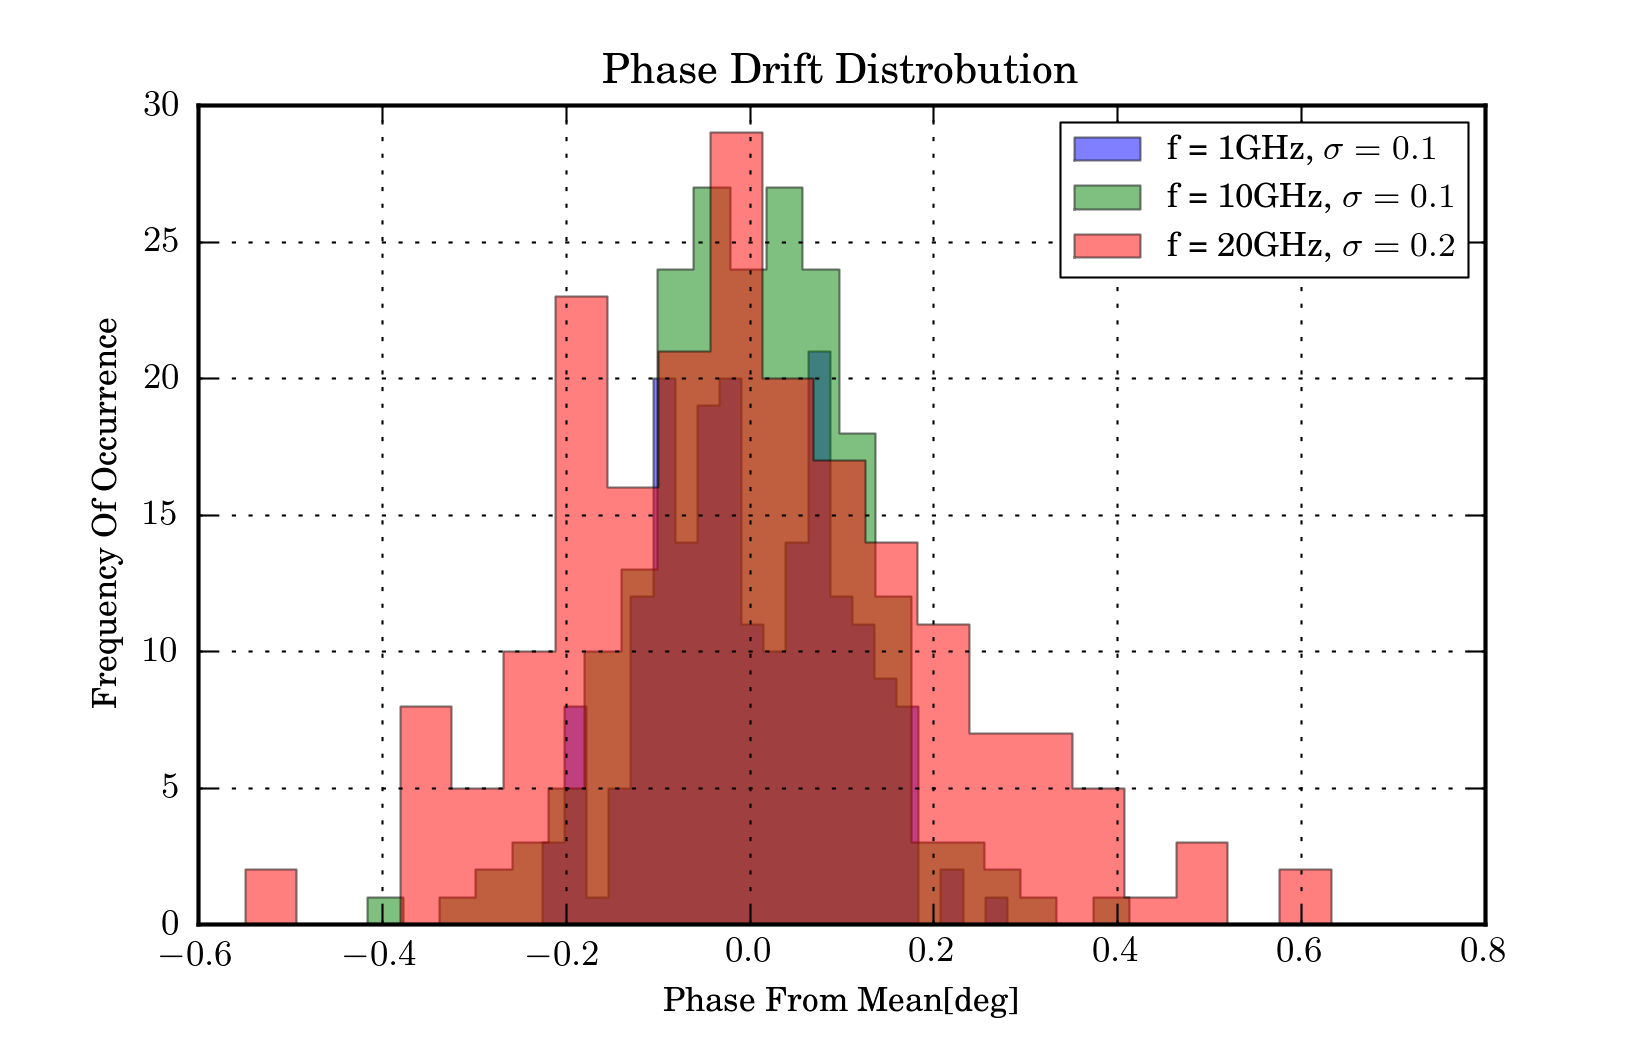
\includegraphics{PhaseDriftDistrobution.png}
\end{figure}
\begin{figure}[htbp]
\centering

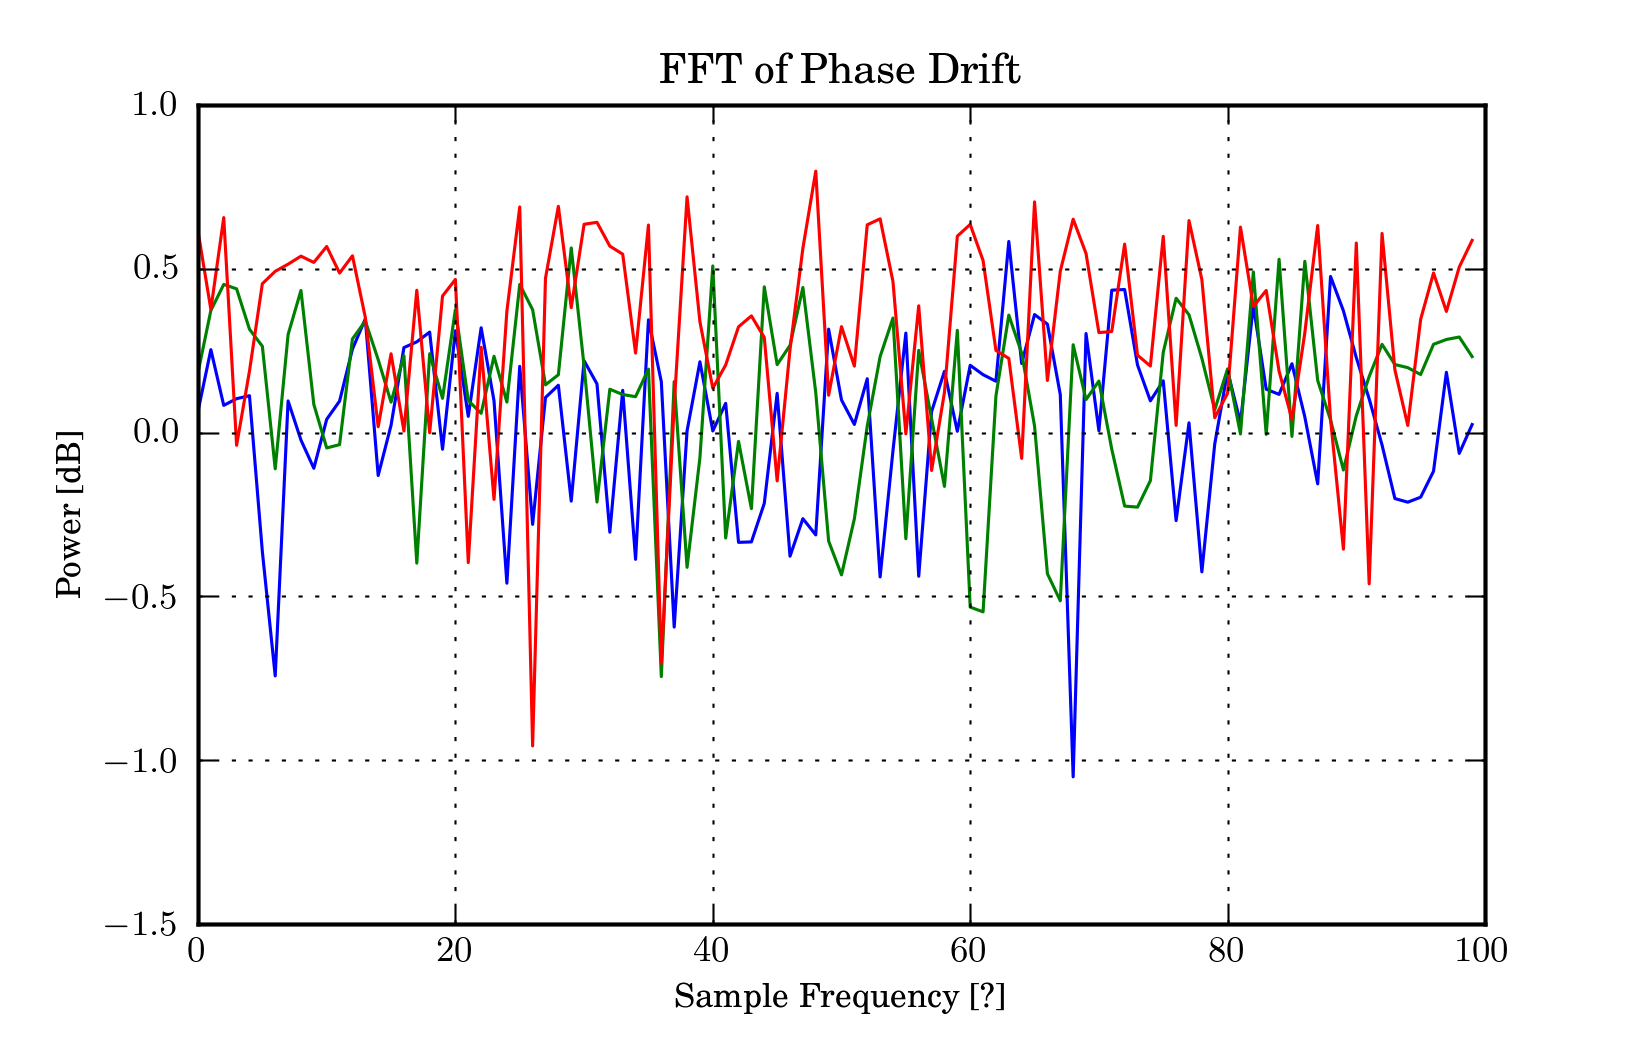
\includegraphics{FFTofPhaseDrift.png}
\end{figure}


\section{Circuit Design: Single Stub Matching Network}
\label{examples/matching_single_stub:example-matching-single-stub}\label{examples/matching_single_stub:circuit-design-single-stub-matching-network}\label{examples/matching_single_stub::doc}

\subsection{Introduction}
\label{examples/matching_single_stub:introduction}
This example illustrates a way to visualize the design space for a single stub matching network. The matching Network consists of a shunt and series stub arranged as shown below, (image taken from R.M. Weikle's Notes)
\begin{figure}[htbp]
\centering

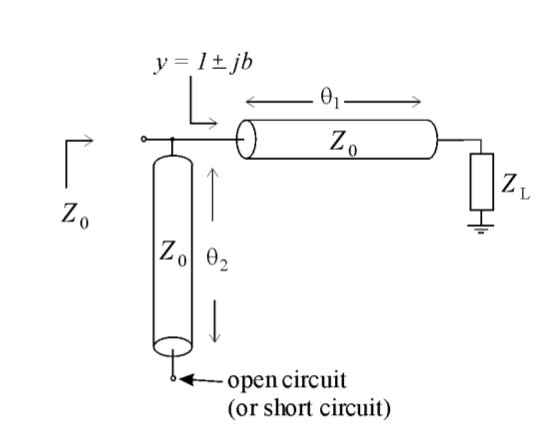
\includegraphics{single_stub_matching_diagram.png}
\end{figure}

A single stub matching network can be designed to produce maximum power transfer to the load, at a single frequency. The matching network has two design parameters:
\begin{itemize}
\item {} 
length of series tline

\item {} 
length of shunt tline

\end{itemize}

This script illustrates how to create a plot of return loss magnitude off the matched load, vs series and shunt line lengths. The optmial designs are then seen as the minima of a 2D surface.


\subsection{Script}
\label{examples/matching_single_stub:script}
\begin{Verbatim}[commandchars=\\\{\}]
\PYG{k+kn}{import} \PYG{n+nn}{mwavepy} \PYG{k+kn}{as} \PYG{n+nn}{mv}
\PYG{k+kn}{from} \PYG{n+nn}{pylab} \PYG{k+kn}{import} \PYG{o}{*}


\PYG{c}{\PYGZsh{} Inputs}
\PYG{n}{wg} \PYG{o}{=} \PYG{n}{mv}\PYG{o}{.}\PYG{n}{wr10} \PYG{c}{\PYGZsh{} The Media class}
\PYG{n}{f0} \PYG{o}{=} \PYG{l+m+mi}{90}                 \PYG{c}{\PYGZsh{} Design Frequency in GHz}
\PYG{n}{d\PYGZus{}start}\PYG{p}{,} \PYG{n}{d\PYGZus{}stop} \PYG{o}{=} \PYG{l+m+mi}{0}\PYG{p}{,}\PYG{l+m+mi}{180} \PYG{c}{\PYGZsh{} span of tline lengths [degrees]}
\PYG{n}{n} \PYG{o}{=} \PYG{l+m+mi}{51}                  \PYG{c}{\PYGZsh{} number of points}
\PYG{n}{Gamma0} \PYG{o}{=} \PYG{o}{.}\PYG{l+m+mi}{5}     \PYG{c}{\PYGZsh{} the reflection coefficient off the load we are matching}


\PYG{c}{\PYGZsh{} change wg.frequency so we only simulat at f0}
\PYG{n}{wg}\PYG{o}{.}\PYG{n}{frequency} \PYG{o}{=} \PYG{n}{mv}\PYG{o}{.}\PYG{n}{Frequency}\PYG{p}{(}\PYG{n}{f0}\PYG{p}{,}\PYG{n}{f0}\PYG{p}{,}\PYG{l+m+mi}{1}\PYG{p}{,}\PYG{l+s}{'}\PYG{l+s}{ghz}\PYG{l+s}{'}\PYG{p}{)}
\PYG{c}{\PYGZsh{} create load network}
\PYG{n}{load} \PYG{o}{=} \PYG{n}{wg}\PYG{o}{.}\PYG{n}{load}\PYG{p}{(}\PYG{o}{.}\PYG{l+m+mi}{5}\PYG{p}{)}
\PYG{c}{\PYGZsh{} the vector of possible line-lengths to simulate at}
\PYG{n}{d\PYGZus{}range} \PYG{o}{=} \PYG{n}{linspace}\PYG{p}{(}\PYG{n}{d\PYGZus{}start}\PYG{p}{,}\PYG{n}{d\PYGZus{}stop}\PYG{p}{,}\PYG{n}{n}\PYG{p}{)}

\PYG{k}{def} \PYG{n+nf}{single\PYGZus{}stub}\PYG{p}{(}\PYG{n}{wb}\PYG{p}{,}\PYG{n}{d}\PYG{p}{)}\PYG{p}{:}
        \PYG{l+s+sd}{'''}
\PYG{l+s+sd}{        function to return series-shunt stub matching network, given a}
\PYG{l+s+sd}{        WorkingBand and the electrical lengths of the stubs}
\PYG{l+s+sd}{        '''}
        \PYG{k}{return} \PYG{n}{wg}\PYG{o}{.}\PYG{n}{shunt\PYGZus{}delay\PYGZus{}open}\PYG{p}{(}\PYG{n}{d}\PYG{p}{[}\PYG{l+m+mi}{1}\PYG{p}{]}\PYG{p}{,}\PYG{l+s}{'}\PYG{l+s}{deg}\PYG{l+s}{'}\PYG{p}{)} \PYG{o}{*}\PYG{o}{*} \PYG{n}{wg}\PYG{o}{.}\PYG{n}{line}\PYG{p}{(}\PYG{n}{d}\PYG{p}{[}\PYG{l+m+mi}{0}\PYG{p}{]}\PYG{p}{,}\PYG{l+s}{'}\PYG{l+s}{deg}\PYG{l+s}{'}\PYG{p}{)}

\PYG{c}{\PYGZsh{} loop through all line-lengths for series and shunt tlines, and store}
\PYG{c}{\PYGZsh{} reflection coefficient magnitude in array}
\PYG{n}{output} \PYG{o}{=} \PYG{n}{array}\PYG{p}{(}\PYG{p}{[}\PYG{p}{[} \PYG{p}{(}\PYG{n}{single\PYGZus{}stub}\PYG{p}{(}\PYG{n}{wb}\PYG{p}{,}\PYG{p}{[}\PYG{n}{d0}\PYG{p}{,}\PYG{n}{d1}\PYG{p}{]}\PYG{p}{)}\PYG{o}{*}\PYG{o}{*}\PYG{n}{load}\PYG{p}{)}\PYG{o}{.}\PYG{n}{s\PYGZus{}mag}\PYG{p}{[}\PYG{l+m+mi}{0}\PYG{p}{,}\PYG{l+m+mi}{0}\PYG{p}{,}\PYG{l+m+mi}{0}\PYG{p}{]} \PYGZbs{}
        \PYG{k}{for} \PYG{n}{d0} \PYG{o+ow}{in} \PYG{n}{d\PYGZus{}range}\PYG{p}{]} \PYG{k}{for} \PYG{n}{d1} \PYG{o+ow}{in} \PYG{n}{d\PYGZus{}range}\PYG{p}{]} \PYG{p}{)}


\PYG{c}{\PYGZsh{} show the resultant return loss for the parameters space}
\PYG{n}{figure}\PYG{p}{(}\PYG{p}{)}
\PYG{n}{title}\PYG{p}{(}\PYG{l+s}{'}\PYG{l+s}{Series-Shunt Stub Matching Network Design Space (2D)}\PYG{l+s}{'}\PYG{p}{)}
\PYG{n}{imshow}\PYG{p}{(}\PYG{n}{output}\PYG{p}{)}
\PYG{n}{xlabel}\PYG{p}{(}\PYG{l+s}{'}\PYG{l+s}{Series T-line [deg]}\PYG{l+s}{'}\PYG{p}{)}
\PYG{n}{ylabel}\PYG{p}{(}\PYG{l+s}{'}\PYG{l+s}{Shunt T-line [deg]}\PYG{l+s}{'}\PYG{p}{)}
\PYG{n}{xticks}\PYG{p}{(}\PYG{n+nb}{range}\PYG{p}{(}\PYG{l+m+mi}{0}\PYG{p}{,}\PYG{n}{n}\PYG{o}{+}\PYG{l+m+mi}{1}\PYG{p}{,}\PYG{n}{n}\PYG{o}{/}\PYG{l+m+mi}{5}\PYG{p}{)}\PYG{p}{,}\PYG{n}{d\PYGZus{}range}\PYG{p}{[}\PYG{l+m+mi}{0}\PYG{p}{:}\PYG{p}{:}\PYG{n}{n}\PYG{o}{/}\PYG{l+m+mi}{5}\PYG{p}{]}\PYG{p}{)}
\PYG{n}{yticks}\PYG{p}{(}\PYG{n+nb}{range}\PYG{p}{(}\PYG{l+m+mi}{0}\PYG{p}{,}\PYG{n}{n}\PYG{o}{+}\PYG{l+m+mi}{1}\PYG{p}{,}\PYG{n}{n}\PYG{o}{/}\PYG{l+m+mi}{5}\PYG{p}{)}\PYG{p}{,}\PYG{n}{d\PYGZus{}range}\PYG{p}{[}\PYG{l+m+mi}{0}\PYG{p}{:}\PYG{p}{:}\PYG{n}{n}\PYG{o}{/}\PYG{l+m+mi}{5}\PYG{p}{]}\PYG{p}{)}
\PYG{n}{cbar} \PYG{o}{=} \PYG{n}{colorbar}\PYG{p}{(}\PYG{p}{)}
\PYG{n}{cbar}\PYG{o}{.}\PYG{n}{set\PYGZus{}label}\PYG{p}{(}\PYG{l+s}{'}\PYG{l+s}{Return Loss Magnitude}\PYG{l+s}{'}\PYG{p}{)}

\PYG{k+kn}{from} \PYG{n+nn}{mpl\PYGZus{}toolkits.mplot3d} \PYG{k+kn}{import} \PYG{n}{Axes3D}

\PYG{n}{fig}\PYG{o}{=}\PYG{n}{figure}\PYG{p}{(}\PYG{p}{)}
\PYG{n}{ax} \PYG{o}{=} \PYG{n}{Axes3D}\PYG{p}{(}\PYG{n}{fig}\PYG{p}{)}
\PYG{n}{x}\PYG{p}{,}\PYG{n}{y} \PYG{o}{=} \PYG{n}{meshgrid}\PYG{p}{(}\PYG{n}{d\PYGZus{}range}\PYG{p}{,} \PYG{n}{d\PYGZus{}range}\PYG{p}{)}
\PYG{n}{ax}\PYG{o}{.}\PYG{n}{plot\PYGZus{}surface}\PYG{p}{(}\PYG{n}{x}\PYG{p}{,}\PYG{n}{y}\PYG{p}{,}\PYG{n}{output}\PYG{p}{,} \PYG{n}{rstride}\PYG{o}{=}\PYG{l+m+mi}{1}\PYG{p}{,} \PYG{n}{cstride}\PYG{o}{=}\PYG{l+m+mi}{1}\PYG{p}{,}\PYG{n}{cmap}\PYG{o}{=}\PYG{n}{cm}\PYG{o}{.}\PYG{n}{jet}\PYG{p}{)}
\PYG{n}{ax}\PYG{o}{.}\PYG{n}{set\PYGZus{}xlabel}\PYG{p}{(}\PYG{l+s}{'}\PYG{l+s}{Series T-line [deg]}\PYG{l+s}{'}\PYG{p}{)}
\PYG{n}{ax}\PYG{o}{.}\PYG{n}{set\PYGZus{}ylabel}\PYG{p}{(}\PYG{l+s}{'}\PYG{l+s}{Shunt T-line[deg]}\PYG{l+s}{'}\PYG{p}{)}
\PYG{n}{ax}\PYG{o}{.}\PYG{n}{set\PYGZus{}zlabel}\PYG{p}{(}\PYG{l+s}{'}\PYG{l+s}{Return Loss Magnitude}\PYG{l+s}{'}\PYG{p}{)}
\PYG{n}{ax}\PYG{o}{.}\PYG{n}{set\PYGZus{}title}\PYG{p}{(}\PYG{l+s}{r'}\PYG{l+s}{Series-Shunt Stub Matching Network Design Space (3D)}\PYG{l+s}{'}\PYG{p}{)}
\PYG{n}{draw}\PYG{p}{(}\PYG{p}{)}
\PYG{n}{show}\PYG{p}{(}\PYG{p}{)}
\end{Verbatim}


\subsection{Output}
\label{examples/matching_single_stub:output}\begin{figure}[htbp]
\centering

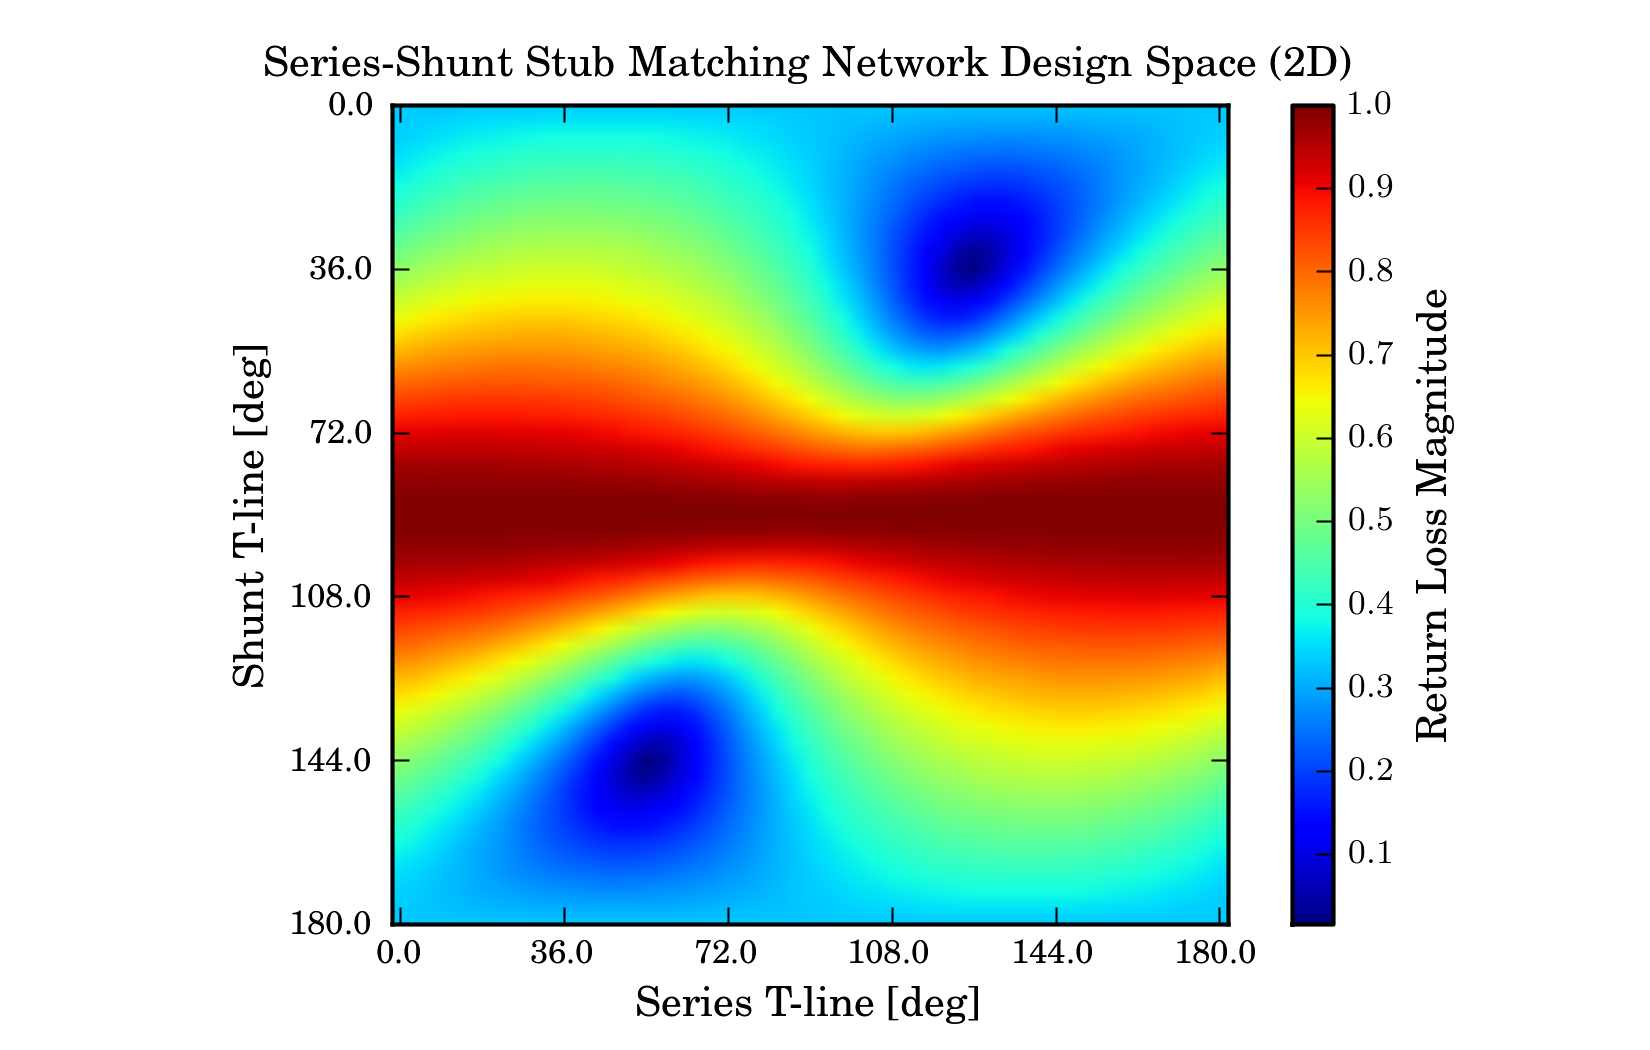
\includegraphics{Series-Shunt_Stub_Matching_2D.png}
\end{figure}
\begin{figure}[htbp]
\centering

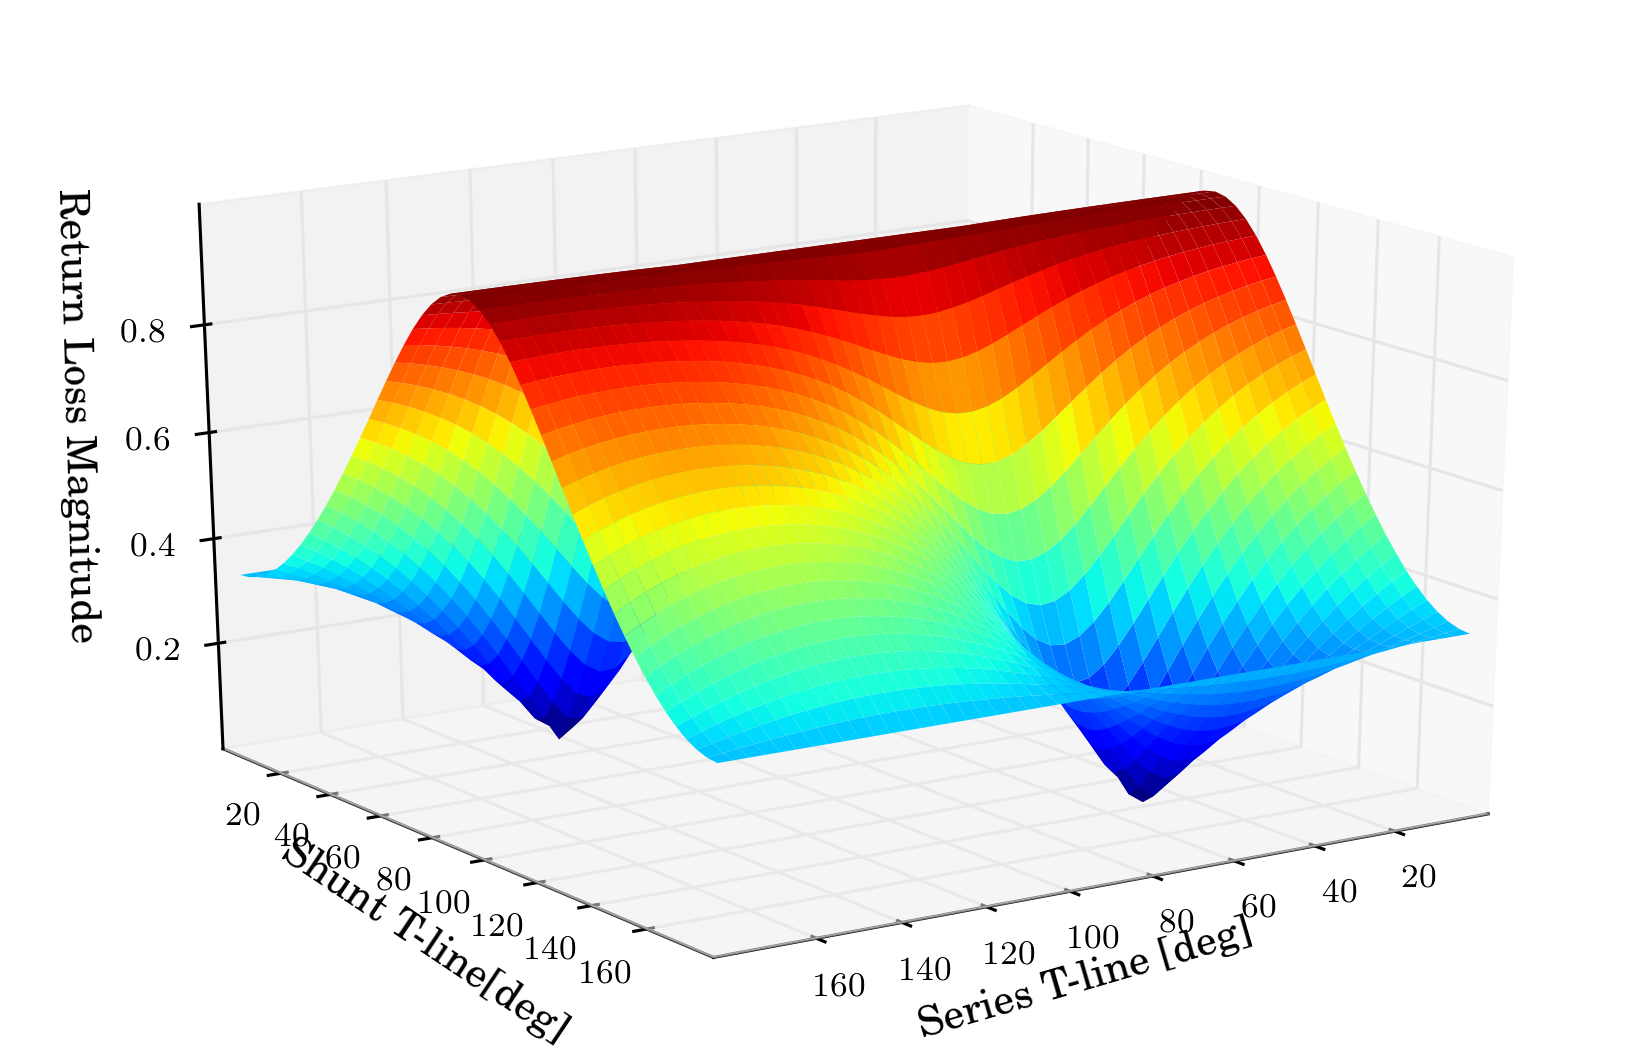
\includegraphics{Series-Shunt_Stub_Matching_3D.png}
\end{figure}

Reference:


\chapter{mwavepy API}
\label{api/modules::doc}\label{api/modules:mwavepy-api}

\section{mwavepy Package}
\label{api/mwavepy:mwavepy-package}\label{api/mwavepy::doc}

\subsection{\texttt{mwavepy} Package}
\label{api/mwavepy:id1}\phantomsection\label{api/mwavepy:module-mwavepy.__init__}\index{mwavepy.\_\_init\_\_ (module)}
mwavepy is an object-oriented approach to microwave engineering, 
implemented in the Python programming language. It provides a set of 
objects and features which can be used to build powerful solutions to 
specific problems. mwavepy's abilities are; touchstone file manipulation,
calibration, VNA data acquisition, circuit design and much more.

This is the main module file for mwavepy. it simply imports classes and
methods. It does this in two ways; import all into the current namespace,
and import modules themselves for coherent  structured referencing


\subsection{\texttt{convenience} Module}
\label{api/mwavepy:convenience-module}\label{api/mwavepy:module-mwavepy.convenience}\index{mwavepy.convenience (module)}
Holds pre-initialized  class's to provide convenience. Also provides
some functions, which cant be categorized as anything better than 
general conviniencies.
\begin{quote}
\begin{description}
\item[{Pre-initialized classes include:}] \leavevmode
Frequency Objects for standard frequency bands
Media objects for standard waveguide bands,

\end{description}
\end{quote}
\index{find\_nearest() (in module mwavepy.convenience)}

\begin{fulllineitems}
\phantomsection\label{api/mwavepy:mwavepy.convenience.find_nearest}\pysiglinewithargsret{\code{mwavepy.convenience.}\bfcode{find\_nearest}}{\emph{array}, \emph{value}}{}
find nearest value in array.
taken from  \href{http://stackoverflow.com/questions/2566412/find-nearest-value-in-numpy-array}{http://stackoverflow.com/questions/2566412/find-nearest-value-in-numpy-array}

\end{fulllineitems}

\index{find\_nearest\_index() (in module mwavepy.convenience)}

\begin{fulllineitems}
\phantomsection\label{api/mwavepy:mwavepy.convenience.find_nearest_index}\pysiglinewithargsret{\code{mwavepy.convenience.}\bfcode{find\_nearest\_index}}{\emph{array}, \emph{value}}{}
find nearest value in array.
taken from  \href{http://stackoverflow.com/questions/2566412/find-nearest-value-in-numpy-array}{http://stackoverflow.com/questions/2566412/find-nearest-value-in-numpy-array}

\end{fulllineitems}

\index{legend\_off() (in module mwavepy.convenience)}

\begin{fulllineitems}
\phantomsection\label{api/mwavepy:mwavepy.convenience.legend_off}\pysiglinewithargsret{\code{mwavepy.convenience.}\bfcode{legend\_off}}{\emph{ax=None}}{}
turn off the legend for a given axes. if no axes is given then 
it will use current axes.

\end{fulllineitems}

\index{now\_string() (in module mwavepy.convenience)}

\begin{fulllineitems}
\phantomsection\label{api/mwavepy:mwavepy.convenience.now_string}\pysiglinewithargsret{\code{mwavepy.convenience.}\bfcode{now\_string}}{}{}
\end{fulllineitems}

\index{plot\_complex() (in module mwavepy.convenience)}

\begin{fulllineitems}
\phantomsection\label{api/mwavepy:mwavepy.convenience.plot_complex}\pysiglinewithargsret{\code{mwavepy.convenience.}\bfcode{plot\_complex}}{\emph{z}, \emph{*args}, \emph{**kwargs}}{}
plots a complex array or list in real vs imaginary.

\end{fulllineitems}

\index{save\_all\_figs() (in module mwavepy.convenience)}

\begin{fulllineitems}
\phantomsection\label{api/mwavepy:mwavepy.convenience.save_all_figs}\pysiglinewithargsret{\code{mwavepy.convenience.}\bfcode{save\_all\_figs}}{\emph{dir='./'}, \emph{format=}\optional{, \emph{`eps'}, \emph{`pdf'}, \emph{`png'}}}{}
\end{fulllineitems}



\subsection{\texttt{frequency} Module}
\label{api/mwavepy:module-mwavepy.frequency}\label{api/mwavepy:frequency-module}\index{mwavepy.frequency (module)}
Provides the Frequency class, and related functions
\index{Frequency (class in mwavepy.frequency)}

\begin{fulllineitems}
\phantomsection\label{api/mwavepy:mwavepy.frequency.Frequency}\pysiglinewithargsret{\strong{class }\code{mwavepy.frequency.}\bfcode{Frequency}}{\emph{start}, \emph{stop}, \emph{npoints}, \emph{unit='hz'}, \emph{sweep\_type='lin'}}{}
Bases: \code{object}

represents a frequency band.
\begin{description}
\item[{attributes:}] \leavevmode
start: starting frequency  (in Hz)
stop: stoping frequency  (in Hz)
npoints: number of points, an int
unit: unit which to scale a formated axis, when accesssed. see
\begin{quote}

formattedAxis
\end{quote}

\end{description}

frequently many calcluations are made in a given band , so this class 
is used in other classes so user doesnt have to continually supply 
frequency info.
\index{center (mwavepy.frequency.Frequency attribute)}

\begin{fulllineitems}
\phantomsection\label{api/mwavepy:mwavepy.frequency.Frequency.center}\pysigline{\bfcode{center}}{}
\end{fulllineitems}

\index{f (mwavepy.frequency.Frequency attribute)}

\begin{fulllineitems}
\phantomsection\label{api/mwavepy:mwavepy.frequency.Frequency.f}\pysigline{\bfcode{f}}{}
returns a frequency vector  in Hz

\end{fulllineitems}

\index{f\_scaled (mwavepy.frequency.Frequency attribute)}

\begin{fulllineitems}
\phantomsection\label{api/mwavepy:mwavepy.frequency.Frequency.f_scaled}\pysigline{\bfcode{f\_scaled}}{}
returns a frequency vector in units of self.unit

\end{fulllineitems}

\index{from\_f() (mwavepy.frequency.Frequency class method)}

\begin{fulllineitems}
\phantomsection\label{api/mwavepy:mwavepy.frequency.Frequency.from_f}\pysiglinewithargsret{\strong{classmethod }\bfcode{from\_f}}{\emph{f}, \emph{*args}, \emph{**kwargs}}{}
alternative constructor from a frequency vector,
takes:
\begin{quote}

f: frequency array (default in Hz)
\end{quote}
\begin{description}
\item[{returns:}] \leavevmode
mwavepy.Frequency object

\end{description}

\end{fulllineitems}

\index{labelXAxis() (mwavepy.frequency.Frequency method)}

\begin{fulllineitems}
\phantomsection\label{api/mwavepy:mwavepy.frequency.Frequency.labelXAxis}\pysiglinewithargsret{\bfcode{labelXAxis}}{\emph{ax=None}}{}
\end{fulllineitems}

\index{multiplier (mwavepy.frequency.Frequency attribute)}

\begin{fulllineitems}
\phantomsection\label{api/mwavepy:mwavepy.frequency.Frequency.multiplier}\pysigline{\bfcode{multiplier}}{}
multiplier for formating axis

\end{fulllineitems}

\index{unit (mwavepy.frequency.Frequency attribute)}

\begin{fulllineitems}
\phantomsection\label{api/mwavepy:mwavepy.frequency.Frequency.unit}\pysigline{\bfcode{unit}}{}
The unit to format the frequency axis in. see formatedAxis

\end{fulllineitems}

\index{w (mwavepy.frequency.Frequency attribute)}

\begin{fulllineitems}
\phantomsection\label{api/mwavepy:mwavepy.frequency.Frequency.w}\pysigline{\bfcode{w}}{}
angular frequency in radians

\end{fulllineitems}


\end{fulllineitems}

\index{f\_2\_frequency() (in module mwavepy.frequency)}

\begin{fulllineitems}
\phantomsection\label{api/mwavepy:mwavepy.frequency.f_2_frequency}\pysiglinewithargsret{\code{mwavepy.frequency.}\bfcode{f\_2\_frequency}}{\emph{f}}{}
convienience function
converts a frequency vector to a Frequency object

!depricated, use classmethod from\_f instead.

\end{fulllineitems}



\subsection{\texttt{mathFunctions} Module}
\label{api/mwavepy:module-mwavepy.mathFunctions}\label{api/mwavepy:mathfunctions-module}\index{mwavepy.mathFunctions (module)}
Provides commonly used math functions.
\index{complex2MagPhase() (in module mwavepy.mathFunctions)}

\begin{fulllineitems}
\phantomsection\label{api/mwavepy:mwavepy.mathFunctions.complex2MagPhase}\pysiglinewithargsret{\code{mwavepy.mathFunctions.}\bfcode{complex2MagPhase}}{\emph{complx}, \emph{deg=False}}{}
\end{fulllineitems}

\index{complex2ReIm() (in module mwavepy.mathFunctions)}

\begin{fulllineitems}
\phantomsection\label{api/mwavepy:mwavepy.mathFunctions.complex2ReIm}\pysiglinewithargsret{\code{mwavepy.mathFunctions.}\bfcode{complex2ReIm}}{\emph{complx}}{}
\end{fulllineitems}

\index{complex2Scalar() (in module mwavepy.mathFunctions)}

\begin{fulllineitems}
\phantomsection\label{api/mwavepy:mwavepy.mathFunctions.complex2Scalar}\pysiglinewithargsret{\code{mwavepy.mathFunctions.}\bfcode{complex2Scalar}}{\emph{input}}{}
\end{fulllineitems}

\index{complex2dB() (in module mwavepy.mathFunctions)}

\begin{fulllineitems}
\phantomsection\label{api/mwavepy:mwavepy.mathFunctions.complex2dB}\pysiglinewithargsret{\code{mwavepy.mathFunctions.}\bfcode{complex2dB}}{\emph{complx}}{}
\end{fulllineitems}

\index{complex\_2\_db() (in module mwavepy.mathFunctions)}

\begin{fulllineitems}
\phantomsection\label{api/mwavepy:mwavepy.mathFunctions.complex_2_db}\pysiglinewithargsret{\code{mwavepy.mathFunctions.}\bfcode{complex\_2\_db}}{\emph{input}}{}
returns the magnitude in dB of a complex number.
\begin{description}
\item[{returns:}] \leavevmode
20*log10({\color{red}\bfseries{}\textbar{}z\textbar{}})

\end{description}

where z is a complex number

\end{fulllineitems}

\index{complex\_2\_degree() (in module mwavepy.mathFunctions)}

\begin{fulllineitems}
\phantomsection\label{api/mwavepy:mwavepy.mathFunctions.complex_2_degree}\pysiglinewithargsret{\code{mwavepy.mathFunctions.}\bfcode{complex\_2\_degree}}{\emph{input}}{}
returns the angle complex number in radians.

\end{fulllineitems}

\index{complex\_2\_magnitude() (in module mwavepy.mathFunctions)}

\begin{fulllineitems}
\phantomsection\label{api/mwavepy:mwavepy.mathFunctions.complex_2_magnitude}\pysiglinewithargsret{\code{mwavepy.mathFunctions.}\bfcode{complex\_2\_magnitude}}{\emph{input}}{}
returns the magnitude of a complex number.

\end{fulllineitems}

\index{complex\_2\_quadrature() (in module mwavepy.mathFunctions)}

\begin{fulllineitems}
\phantomsection\label{api/mwavepy:mwavepy.mathFunctions.complex_2_quadrature}\pysiglinewithargsret{\code{mwavepy.mathFunctions.}\bfcode{complex\_2\_quadrature}}{\emph{z}}{}
takes a complex number and returns quadrature, which is (length, arc-length from real axis)

\end{fulllineitems}

\index{complex\_2\_radian() (in module mwavepy.mathFunctions)}

\begin{fulllineitems}
\phantomsection\label{api/mwavepy:mwavepy.mathFunctions.complex_2_radian}\pysiglinewithargsret{\code{mwavepy.mathFunctions.}\bfcode{complex\_2\_radian}}{\emph{input}}{}
returns the angle complex number in radians.

\end{fulllineitems}

\index{complex\_components() (in module mwavepy.mathFunctions)}

\begin{fulllineitems}
\phantomsection\label{api/mwavepy:mwavepy.mathFunctions.complex_components}\pysiglinewithargsret{\code{mwavepy.mathFunctions.}\bfcode{complex\_components}}{\emph{z}}{}
break up a complex array into all possible scalar components

takes: complex ndarray 
return:
\begin{quote}

c\_real: real part
c\_imag: imaginary part
c\_angle: angle in degrees
c\_mag:  magnitude
c\_arc:  arclength from real axis, angle*magnitude
\end{quote}

\end{fulllineitems}

\index{db\_2\_magnitude() (in module mwavepy.mathFunctions)}

\begin{fulllineitems}
\phantomsection\label{api/mwavepy:mwavepy.mathFunctions.db_2_magnitude}\pysiglinewithargsret{\code{mwavepy.mathFunctions.}\bfcode{db\_2\_magnitude}}{\emph{input}}{}
converts db to normal magnitude
\begin{description}
\item[{returns:}] \leavevmode
10**((z)/20.)

\end{description}

where z is a complex number

\end{fulllineitems}

\index{db\_2\_np() (in module mwavepy.mathFunctions)}

\begin{fulllineitems}
\phantomsection\label{api/mwavepy:mwavepy.mathFunctions.db_2_np}\pysiglinewithargsret{\code{mwavepy.mathFunctions.}\bfcode{db\_2\_np}}{\emph{x}}{}
converts a value in nepers to dB

\end{fulllineitems}

\index{degree\_2\_radian() (in module mwavepy.mathFunctions)}

\begin{fulllineitems}
\phantomsection\label{api/mwavepy:mwavepy.mathFunctions.degree_2_radian}\pysiglinewithargsret{\code{mwavepy.mathFunctions.}\bfcode{degree\_2\_radian}}{\emph{deg}}{}
\end{fulllineitems}

\index{dirac\_delta() (in module mwavepy.mathFunctions)}

\begin{fulllineitems}
\phantomsection\label{api/mwavepy:mwavepy.mathFunctions.dirac_delta}\pysiglinewithargsret{\code{mwavepy.mathFunctions.}\bfcode{dirac\_delta}}{\emph{x}}{}
the dirac function.

can take numpy arrays or numbers
returns 1 or 0

\end{fulllineitems}

\index{magnitude\_2\_db() (in module mwavepy.mathFunctions)}

\begin{fulllineitems}
\phantomsection\label{api/mwavepy:mwavepy.mathFunctions.magnitude_2_db}\pysiglinewithargsret{\code{mwavepy.mathFunctions.}\bfcode{magnitude\_2\_db}}{\emph{input}}{}
converts magnitude to db
\begin{quote}
\begin{description}
\item[{db is given by }] \leavevmode
20*log10({\color{red}\bfseries{}\textbar{}z\textbar{}})

\end{description}
\end{quote}

where z is a complex number

\end{fulllineitems}

\index{neuman() (in module mwavepy.mathFunctions)}

\begin{fulllineitems}
\phantomsection\label{api/mwavepy:mwavepy.mathFunctions.neuman}\pysiglinewithargsret{\code{mwavepy.mathFunctions.}\bfcode{neuman}}{\emph{x}}{}
neumans number

2-dirac\_delta(x)

\end{fulllineitems}

\index{np\_2\_db() (in module mwavepy.mathFunctions)}

\begin{fulllineitems}
\phantomsection\label{api/mwavepy:mwavepy.mathFunctions.np_2_db}\pysiglinewithargsret{\code{mwavepy.mathFunctions.}\bfcode{np\_2\_db}}{\emph{x}}{}
converts a value in dB to neper's

\end{fulllineitems}

\index{null() (in module mwavepy.mathFunctions)}

\begin{fulllineitems}
\phantomsection\label{api/mwavepy:mwavepy.mathFunctions.null}\pysiglinewithargsret{\code{mwavepy.mathFunctions.}\bfcode{null}}{\emph{A}, \emph{eps=1e-15}}{}~\begin{quote}

calculates the null space of matrix A.
\end{quote}

i found this on stack overflow.

\end{fulllineitems}

\index{psd2TimeDomain() (in module mwavepy.mathFunctions)}

\begin{fulllineitems}
\phantomsection\label{api/mwavepy:mwavepy.mathFunctions.psd2TimeDomain}\pysiglinewithargsret{\code{mwavepy.mathFunctions.}\bfcode{psd2TimeDomain}}{\emph{f}, \emph{y}, \emph{windowType='hamming'}}{}
convert a one sided complex spectrum into a real time-signal.
takes
\begin{quote}

f: frequency array, 
y: complex PSD arary 
windowType: windowing function, defaults to rect
\end{quote}
\begin{description}
\item[{returns in the form:}] \leavevmode
{[}timeVector, signalVector{]}

\end{description}

timeVector is in inverse units of the input variable f,
if spectrum is not baseband then, timeSignal is modulated by
\begin{quote}

exp(t*2*pi*f{[}0{]})
\end{quote}

so keep in mind units, also due to this f must be increasing left to right

\end{fulllineitems}

\index{radian\_2\_degree() (in module mwavepy.mathFunctions)}

\begin{fulllineitems}
\phantomsection\label{api/mwavepy:mwavepy.mathFunctions.radian_2_degree}\pysiglinewithargsret{\code{mwavepy.mathFunctions.}\bfcode{radian\_2\_degree}}{\emph{rad}}{}
\end{fulllineitems}

\index{scalar2Complex() (in module mwavepy.mathFunctions)}

\begin{fulllineitems}
\phantomsection\label{api/mwavepy:mwavepy.mathFunctions.scalar2Complex}\pysiglinewithargsret{\code{mwavepy.mathFunctions.}\bfcode{scalar2Complex}}{\emph{input}}{}
\end{fulllineitems}



\subsection{\texttt{network} Module}
\label{api/mwavepy:module-mwavepy.network}\label{api/mwavepy:network-module}\index{mwavepy.network (module)}
Provides the Network class and related functions.
\index{Network (class in mwavepy.network)}

\begin{fulllineitems}
\phantomsection\label{api/mwavepy:mwavepy.network.Network}\pysiglinewithargsret{\strong{class }\code{mwavepy.network.}\bfcode{Network}}{\emph{touchstone\_file=None}, \emph{name=None}}{}
Bases: \code{object}

Represents a n-port microwave network.
\begin{description}
\item[{the most fundemental properties are:}] \leavevmode\begin{description}
\item[{s: scattering matrix. a kxnxn complex matrix where `n' is number}] \leavevmode
of ports of network.

\end{description}

z0: characteristic impedance
f: frequency vector in Hz. see also frequency, which is a
\begin{quote}

Frequency object (see help on this class for more info)
\end{quote}

\item[{The following operators are defined as follows:}] \leavevmode
`+' : element-wise addition of the s-matrix
`-` : element-wise subtraction of the s-matrix
`*' : element-wise multiplication of the s-matrix
`/' : element-wise division of the s-matrix
`**': cascading of 2-port networks
`//': de-embdeding of one network from the other.

\end{description}

various other network properties are accesable as well as plotting
routines are also defined for convenience,

most properties are derived from the specifications given for
touchstone files.
\index{add\_noise\_polar() (mwavepy.network.Network method)}

\begin{fulllineitems}
\phantomsection\label{api/mwavepy:mwavepy.network.Network.add_noise_polar}\pysiglinewithargsret{\bfcode{add\_noise\_polar}}{\emph{mag\_dev}, \emph{phase\_dev}, \emph{**kwargs}}{}
adds a complex zero-mean gaussian white-noise signal of given
standard deviations for magnitude and phase
\begin{description}
\item[{takes:}] \leavevmode
mag\_mag: standard deviation of magnitude
phase\_dev: standard deviation of phase {[}in degrees{]}
n\_ports: number of ports. defualt to 1

\item[{returns:}] \leavevmode
nothing

\end{description}

\end{fulllineitems}

\index{add\_noise\_polar\_flatband() (mwavepy.network.Network method)}

\begin{fulllineitems}
\phantomsection\label{api/mwavepy:mwavepy.network.Network.add_noise_polar_flatband}\pysiglinewithargsret{\bfcode{add\_noise\_polar\_flatband}}{\emph{mag\_dev}, \emph{phase\_dev}, \emph{**kwargs}}{}
adds a flatband complex zero-mean gaussian white-noise signal of
given standard deviations for magnitude and phase
\begin{description}
\item[{takes:}] \leavevmode
mag\_mag: standard deviation of magnitude
phase\_dev: standard deviation of phase {[}in degrees{]}
n\_ports: number of ports. defualt to 1

\item[{returns:}] \leavevmode
nothing

\end{description}

\end{fulllineitems}

\index{change\_frequency() (mwavepy.network.Network method)}

\begin{fulllineitems}
\phantomsection\label{api/mwavepy:mwavepy.network.Network.change_frequency}\pysiglinewithargsret{\bfcode{change\_frequency}}{\emph{new\_frequency}, \emph{**kwargs}}{}
\end{fulllineitems}

\index{f (mwavepy.network.Network attribute)}

\begin{fulllineitems}
\phantomsection\label{api/mwavepy:mwavepy.network.Network.f}\pysigline{\bfcode{f}}{}
the frequency vector for the network, in Hz.

\end{fulllineitems}

\index{flip() (mwavepy.network.Network method)}

\begin{fulllineitems}
\phantomsection\label{api/mwavepy:mwavepy.network.Network.flip}\pysiglinewithargsret{\bfcode{flip}}{}{}
swaps the ports of a two port

\end{fulllineitems}

\index{frequency (mwavepy.network.Network attribute)}

\begin{fulllineitems}
\phantomsection\label{api/mwavepy:mwavepy.network.Network.frequency}\pysigline{\bfcode{frequency}}{}
returns a Frequency object, see  frequency.py

\end{fulllineitems}

\index{interpolate() (mwavepy.network.Network method)}

\begin{fulllineitems}
\phantomsection\label{api/mwavepy:mwavepy.network.Network.interpolate}\pysiglinewithargsret{\bfcode{interpolate}}{\emph{new\_frequency}, \emph{**kwargs}}{}
calculates an interpolated network. defualt interpolation type
is linear. see notes about other interpolation types
\begin{description}
\item[{takes:}] \leavevmode
new\_frequency:
{\color{red}\bfseries{}**}kwargs: passed to scipy.interpolate.interp1d initializer.

\item[{returns:}] \leavevmode
result: an interpolated Network

\item[{note:}] \leavevmode\begin{description}
\item[{usefule keyward for  scipy.interpolate.interp1d:}] \leavevmode\begin{description}
\item[{kind}] \leavevmode{[}str or int{]}
Specifies the kind of interpolation as a string (`linear',
`nearest', `zero', `slinear', `quadratic, `cubic') or as an integer
specifying the order of the spline interpolator to use.

\end{description}

\end{description}

\end{description}

\end{fulllineitems}

\index{inv (mwavepy.network.Network attribute)}

\begin{fulllineitems}
\phantomsection\label{api/mwavepy:mwavepy.network.Network.inv}\pysigline{\bfcode{inv}}{}
a network representing inverse s-parameters, for de-embeding

\end{fulllineitems}

\index{multiply\_noise() (mwavepy.network.Network method)}

\begin{fulllineitems}
\phantomsection\label{api/mwavepy:mwavepy.network.Network.multiply_noise}\pysiglinewithargsret{\bfcode{multiply\_noise}}{\emph{mag\_dev}, \emph{phase\_dev}, \emph{**kwargs}}{}
multiplys a complex bivariate gaussian white-noise signal
of given standard deviations for magnitude and phase.   
magnitude mean is 1, phase mean is 0
\begin{description}
\item[{takes:}] \leavevmode
mag\_dev: standard deviation of magnitude
phase\_dev: standard deviation of phase {[}in degrees{]}
n\_ports: number of ports. defualt to 1

\item[{returns:}] \leavevmode
nothing

\end{description}

\end{fulllineitems}

\index{nudge() (mwavepy.network.Network method)}

\begin{fulllineitems}
\phantomsection\label{api/mwavepy:mwavepy.network.Network.nudge}\pysiglinewithargsret{\bfcode{nudge}}{\emph{amount=1e-12}}{}
perturb s-parameters by small amount. this is usefule to work-around
numerical bugs.
takes:
\begin{quote}

amount: amount to add to s parameters
\end{quote}
\begin{description}
\item[{returns:}] \leavevmode
na

\end{description}

\end{fulllineitems}

\index{number\_of\_ports (mwavepy.network.Network attribute)}

\begin{fulllineitems}
\phantomsection\label{api/mwavepy:mwavepy.network.Network.number_of_ports}\pysigline{\bfcode{number\_of\_ports}}{}
the number of ports the network has.

\end{fulllineitems}

\index{passivity (mwavepy.network.Network attribute)}

\begin{fulllineitems}
\phantomsection\label{api/mwavepy:mwavepy.network.Network.passivity}\pysigline{\bfcode{passivity}}{}~\begin{quote}

passivity metric for a multi-port network. It returns
\end{quote}

a matrix who's diagonals are equal to the total power 
received at all ports, normalized to the power at a single
excitement  port.

mathmatically, this is a test for unitary-ness of the 
s-parameter matrix.
\begin{description}
\item[{for two port this is }] \leavevmode
( {\color{red}\bfseries{}\textbar{}}S11\textbar{}\textasciicircum{}2 + {\color{red}\bfseries{}\textbar{}}S21\textbar{}\textasciicircum{}2, {\color{red}\bfseries{}\textbar{}}S22\textbar{}\textasciicircum{}2+\textbar{}S12\textbar{}\textasciicircum{}2)

\item[{in general it is  }] \leavevmode
S.H * S

\end{description}

where H is conjugate transpose of S, and * is dot product

note:
see more at,
\href{http://en.wikipedia.org/wiki/Scattering\_parameters\#Lossless\_networks}{http://en.wikipedia.org/wiki/Scattering\_parameters\#Lossless\_networks}

\end{fulllineitems}

\index{plot\_polar\_generic() (mwavepy.network.Network method)}

\begin{fulllineitems}
\phantomsection\label{api/mwavepy:mwavepy.network.Network.plot_polar_generic}\pysiglinewithargsret{\bfcode{plot\_polar\_generic}}{\emph{attribute\_r}, \emph{attribute\_theta}, \emph{m=0}, \emph{n=0}, \emph{ax=None}, \emph{show\_legend=True}, \emph{**kwargs}}{}
generic plotting function for plotting a Network's attribute
in polar form

takes:

\end{fulllineitems}

\index{plot\_s\_all\_db() (mwavepy.network.Network method)}

\begin{fulllineitems}
\phantomsection\label{api/mwavepy:mwavepy.network.Network.plot_s_all_db}\pysiglinewithargsret{\bfcode{plot\_s\_all\_db}}{\emph{ax=None}, \emph{show\_legend=True}, \emph{*args}, \emph{**kwargs}}{}
plots all s parameters in log magnitude
\begin{description}
\item[{takes:}] \leavevmode\begin{description}
\item[{ax - matplotlib.axes object to plot on, used in case you}] \leavevmode
want to update an existing plot.

\end{description}

show\_legend: boolean, to turn legend show legend of not
{\color{red}\bfseries{}*}args,**kwargs - passed to the matplotlib.plot command

\end{description}

\end{fulllineitems}

\index{plot\_s\_complex() (mwavepy.network.Network method)}

\begin{fulllineitems}
\phantomsection\label{api/mwavepy:mwavepy.network.Network.plot_s_complex}\pysiglinewithargsret{\bfcode{plot\_s\_complex}}{\emph{m=None}, \emph{n=None}, \emph{ax=None}, \emph{show\_legend=True}, \emph{*args}, \emph{**kwargs}}{}
plots the scattering parameter of indecies m, n on complex plane
\begin{description}
\item[{takes:}] \leavevmode
m - first index, int
n - second indext, int
ax - matplotlib.axes object to plot on, used in case you
\begin{quote}

want to update an existing plot.
\end{quote}

show\_legend: boolean, to turn legend show legend of not
{\color{red}\bfseries{}*}args,**kwargs - passed to the matplotlib.plot command

\end{description}

\end{fulllineitems}

\index{plot\_s\_db() (mwavepy.network.Network method)}

\begin{fulllineitems}
\phantomsection\label{api/mwavepy:mwavepy.network.Network.plot_s_db}\pysiglinewithargsret{\bfcode{plot\_s\_db}}{\emph{m=None}, \emph{n=None}, \emph{ax=None}, \emph{show\_legend=True}, \emph{*args}, \emph{**kwargs}}{}
plots the magnitude of the scattering parameter of indecies m, n
in log magnitude
\begin{description}
\item[{takes:}] \leavevmode
m - first index, int
n - second indext, int
ax - matplotlib.axes object to plot on, used in case you
\begin{quote}

want to update an existing plot.
\end{quote}

show\_legend: boolean, to turn legend show legend of not
{\color{red}\bfseries{}*}args,**kwargs - passed to the matplotlib.plot command

\end{description}

\end{fulllineitems}

\index{plot\_s\_deg() (mwavepy.network.Network method)}

\begin{fulllineitems}
\phantomsection\label{api/mwavepy:mwavepy.network.Network.plot_s_deg}\pysiglinewithargsret{\bfcode{plot\_s\_deg}}{\emph{m=None}, \emph{n=None}, \emph{ax=None}, \emph{show\_legend=True}, \emph{*args}, \emph{**kwargs}}{}
plots the phase of a scattering parameter of indecies m, n in
degrees
\begin{description}
\item[{takes:}] \leavevmode
m - first index, int
n - second indext, int
ax - matplotlib.axes object to plot on, used in case you
\begin{quote}

want to update an existing plot.
\end{quote}

show\_legend: boolean, to turn legend show legend of not
{\color{red}\bfseries{}*}args,**kwargs - passed to the matplotlib.plot command

\end{description}

\end{fulllineitems}

\index{plot\_s\_deg\_unwrap() (mwavepy.network.Network method)}

\begin{fulllineitems}
\phantomsection\label{api/mwavepy:mwavepy.network.Network.plot_s_deg_unwrap}\pysiglinewithargsret{\bfcode{plot\_s\_deg\_unwrap}}{\emph{m=None}, \emph{n=None}, \emph{ax=None}, \emph{show\_legend=True}, \emph{*args}, \emph{**kwargs}}{}
plots the phase of a scattering parameter of indecies m, n in
unwrapped degrees
\begin{description}
\item[{takes:}] \leavevmode
m - first index, int
n - second indext, int
ax - matplotlib.axes object to plot on, used in case you
\begin{quote}

want to update an existing plot.
\end{quote}

show\_legend: boolean, to turn legend show legend of not
{\color{red}\bfseries{}*}args,**kwargs - passed to the matplotlib.plot command

\end{description}

\end{fulllineitems}

\index{plot\_s\_deg\_unwrapped() (mwavepy.network.Network method)}

\begin{fulllineitems}
\phantomsection\label{api/mwavepy:mwavepy.network.Network.plot_s_deg_unwrapped}\pysiglinewithargsret{\bfcode{plot\_s\_deg\_unwrapped}}{\emph{m=None}, \emph{n=None}, \emph{ax=None}, \emph{show\_legend=True}, \emph{*args}, \emph{**kwargs}}{}
plots the phase of a scattering parameter of indecies m, n in
unwrapped degrees
\begin{description}
\item[{takes:}] \leavevmode
m - first index, int
n - second indext, int
ax - matplotlib.axes object to plot on, used in case you
\begin{quote}

want to update an existing plot.
\end{quote}

show\_legend: boolean, to turn legend show legend of not
{\color{red}\bfseries{}*}args,**kwargs - passed to the matplotlib.plot command

\end{description}

\end{fulllineitems}

\index{plot\_s\_mag() (mwavepy.network.Network method)}

\begin{fulllineitems}
\phantomsection\label{api/mwavepy:mwavepy.network.Network.plot_s_mag}\pysiglinewithargsret{\bfcode{plot\_s\_mag}}{\emph{m=None}, \emph{n=None}, \emph{ax=None}, \emph{show\_legend=True}, \emph{*args}, \emph{**kwargs}}{}
plots the magnitude of a scattering parameter of indecies m, n
not in  magnitude
\begin{description}
\item[{takes:}] \leavevmode
m - first index, int
n - second indext, int
ax - matplotlib.axes object to plot on, used in case you
\begin{quote}

want to update an existing plot.
\end{quote}

show\_legend: boolean, to turn legend show legend of not
{\color{red}\bfseries{}*}args,**kwargs - passed to the matplotlib.plot command

\end{description}

\end{fulllineitems}

\index{plot\_s\_polar() (mwavepy.network.Network method)}

\begin{fulllineitems}
\phantomsection\label{api/mwavepy:mwavepy.network.Network.plot_s_polar}\pysiglinewithargsret{\bfcode{plot\_s\_polar}}{\emph{m=0}, \emph{n=0}, \emph{ax=None}, \emph{show\_legend=True}, \emph{*args}, \emph{**kwargs}}{}
plots the scattering parameter of indecies m, n in polar form
\begin{description}
\item[{takes:}] \leavevmode
m - first index, int
n - second indext, int
ax - matplotlib.axes object to plot on, used in case you
\begin{quote}

want to update an existing plot.
\end{quote}

show\_legend: boolean, to turn legend show legend of not
{\color{red}\bfseries{}*}args,**kwargs - passed to the matplotlib.plot command

\end{description}

\end{fulllineitems}

\index{plot\_s\_rad() (mwavepy.network.Network method)}

\begin{fulllineitems}
\phantomsection\label{api/mwavepy:mwavepy.network.Network.plot_s_rad}\pysiglinewithargsret{\bfcode{plot\_s\_rad}}{\emph{m=None}, \emph{n=None}, \emph{ax=None}, \emph{show\_legend=True}, \emph{*args}, \emph{**kwargs}}{}
plots the phase of a scattering parameter of indecies m, n in
radians
\begin{description}
\item[{takes:}] \leavevmode
m - first index, int
n - second indext, int
ax - matplotlib.axes object to plot on, used in case you
\begin{quote}

want to update an existing plot.
\end{quote}

show\_legend: boolean, to turn legend show legend of not
{\color{red}\bfseries{}*}args,**kwargs - passed to the matplotlib.plot command

\end{description}

\end{fulllineitems}

\index{plot\_s\_rad\_unwrapped() (mwavepy.network.Network method)}

\begin{fulllineitems}
\phantomsection\label{api/mwavepy:mwavepy.network.Network.plot_s_rad_unwrapped}\pysiglinewithargsret{\bfcode{plot\_s\_rad\_unwrapped}}{\emph{m=None}, \emph{n=None}, \emph{ax=None}, \emph{show\_legend=True}, \emph{*args}, \emph{**kwargs}}{}
plots the phase of a scattering parameter of indecies m, n in
unwrapped radians
\begin{description}
\item[{takes:}] \leavevmode
m - first index, int
n - second indext, int
ax - matplotlib.axes object to plot on, used in case you
\begin{quote}

want to update an existing plot.
\end{quote}

show\_legend: boolean, to turn legend show legend of not
{\color{red}\bfseries{}*}args,**kwargs - passed to the matplotlib.plot command

\end{description}

\end{fulllineitems}

\index{plot\_s\_smith() (mwavepy.network.Network method)}

\begin{fulllineitems}
\phantomsection\label{api/mwavepy:mwavepy.network.Network.plot_s_smith}\pysiglinewithargsret{\bfcode{plot\_s\_smith}}{\emph{m=None}, \emph{n=None}, \emph{r=1}, \emph{ax=None}, \emph{show\_legend=True}, \emph{chart\_type='z'}, \emph{*args}, \emph{**kwargs}}{}
plots the scattering parameter of indecies m, n on smith chart
\begin{description}
\item[{takes:}] \leavevmode
m - first index, int
n - second indext, int
r -  radius of smith chart
ax - matplotlib.axes object to plot on, used in case you
\begin{quote}

want to update an existing plot.
\end{quote}

show\_legend: boolean, to turn legend show legend of not
chart\_type: string determining countour type. options are:
\begin{quote}

`z': impedance contours (default)
`y': admittance contours
\end{quote}

{\color{red}\bfseries{}*}args,**kwargs - passed to the matplotlib.plot command

\end{description}

\end{fulllineitems}

\index{plot\_vs\_frequency\_generic() (mwavepy.network.Network method)}

\begin{fulllineitems}
\phantomsection\label{api/mwavepy:mwavepy.network.Network.plot_vs_frequency_generic}\pysiglinewithargsret{\bfcode{plot\_vs\_frequency\_generic}}{\emph{attribute}, \emph{y\_label=None}, \emph{m=None}, \emph{n=None}, \emph{ax=None}, \emph{show\_legend=True}, \emph{**kwargs}}{}
generic plotting function for plotting a Network's attribute
vs frequency.

takes:

\end{fulllineitems}

\index{read\_touchstone() (mwavepy.network.Network method)}

\begin{fulllineitems}
\phantomsection\label{api/mwavepy:mwavepy.network.Network.read_touchstone}\pysiglinewithargsret{\bfcode{read\_touchstone}}{\emph{filename}}{}
loads  values from a touchstone file.
\begin{description}
\item[{takes:}] \leavevmode
filename - touchstone file name, string.

\item[{note: }] \leavevmode
ONLY `S' FORMAT SUPORTED AT THE MOMENT 
all work is tone in the touchstone class.

\end{description}

\end{fulllineitems}

\index{s (mwavepy.network.Network attribute)}

\begin{fulllineitems}
\phantomsection\label{api/mwavepy:mwavepy.network.Network.s}\pysigline{\bfcode{s}}{}
The scattering parameter matrix.

s-matrix has shape fxnxn, 
where;
\begin{quote}

f is frequency axis and,
n's are port indicies
\end{quote}

\end{fulllineitems}

\index{s11 (mwavepy.network.Network attribute)}

\begin{fulllineitems}
\phantomsection\label{api/mwavepy:mwavepy.network.Network.s11}\pysigline{\bfcode{s11}}{}
\end{fulllineitems}

\index{s12 (mwavepy.network.Network attribute)}

\begin{fulllineitems}
\phantomsection\label{api/mwavepy:mwavepy.network.Network.s12}\pysigline{\bfcode{s12}}{}
\end{fulllineitems}

\index{s21 (mwavepy.network.Network attribute)}

\begin{fulllineitems}
\phantomsection\label{api/mwavepy:mwavepy.network.Network.s21}\pysigline{\bfcode{s21}}{}
\end{fulllineitems}

\index{s22 (mwavepy.network.Network attribute)}

\begin{fulllineitems}
\phantomsection\label{api/mwavepy:mwavepy.network.Network.s22}\pysigline{\bfcode{s22}}{}
\end{fulllineitems}

\index{s\_db (mwavepy.network.Network attribute)}

\begin{fulllineitems}
\phantomsection\label{api/mwavepy:mwavepy.network.Network.s_db}\pysigline{\bfcode{s\_db}}{}
returns the magnitude of the s-parameters, in dB
\begin{description}
\item[{note:}] \leavevmode\begin{description}
\item[{dB is calculated by }] \leavevmode
20*log10({\color{red}\bfseries{}\textbar{}s\textbar{}})

\end{description}

\end{description}

\end{fulllineitems}

\index{s\_deg (mwavepy.network.Network attribute)}

\begin{fulllineitems}
\phantomsection\label{api/mwavepy:mwavepy.network.Network.s_deg}\pysigline{\bfcode{s\_deg}}{}
returns the phase of the s-parameters, in radians

\end{fulllineitems}

\index{s\_deg\_unwrap (mwavepy.network.Network attribute)}

\begin{fulllineitems}
\phantomsection\label{api/mwavepy:mwavepy.network.Network.s_deg_unwrap}\pysigline{\bfcode{s\_deg\_unwrap}}{}
returns the unwrapped phase of the s-paramerts, in degrees

\end{fulllineitems}

\index{s\_mag (mwavepy.network.Network attribute)}

\begin{fulllineitems}
\phantomsection\label{api/mwavepy:mwavepy.network.Network.s_mag}\pysigline{\bfcode{s\_mag}}{}
returns the magnitude of the s-parameters.

\end{fulllineitems}

\index{s\_rad (mwavepy.network.Network attribute)}

\begin{fulllineitems}
\phantomsection\label{api/mwavepy:mwavepy.network.Network.s_rad}\pysigline{\bfcode{s\_rad}}{}
returns the phase of the s-parameters, in radians.

\end{fulllineitems}

\index{s\_rad\_unwrap (mwavepy.network.Network attribute)}

\begin{fulllineitems}
\phantomsection\label{api/mwavepy:mwavepy.network.Network.s_rad_unwrap}\pysigline{\bfcode{s\_rad\_unwrap}}{}
returns the unwrapped phase of the s-parameters, in radians.

\end{fulllineitems}

\index{t (mwavepy.network.Network attribute)}

\begin{fulllineitems}
\phantomsection\label{api/mwavepy:mwavepy.network.Network.t}\pysigline{\bfcode{t}}{}
returns the t-parameters, which are also known as wave cascading
matrix.

\end{fulllineitems}

\index{write\_touchstone() (mwavepy.network.Network method)}

\begin{fulllineitems}
\phantomsection\label{api/mwavepy:mwavepy.network.Network.write_touchstone}\pysiglinewithargsret{\bfcode{write\_touchstone}}{\emph{filename=None}, \emph{dir='./'}}{}
write a touchstone file representing this network.  the only 
format supported at the moment is :
\begin{quote}

HZ S RI
\end{quote}
\begin{description}
\item[{takes: }] \leavevmode\begin{description}
\item[{filename: a string containing filename without }] \leavevmode
extension{[}None{]}. if `None', then will use the network's 
name. if this is empty, then throws an error.

\item[{dir: the directory to save the file in. {[}string{]}. Defaults }] \leavevmode
to `./'

\end{description}

\item[{note:}] \leavevmode
in the future could make possible use of the touchtone 
class, but at the moment this would not provide any benefit 
as it has not {\color{red}\bfseries{}set\_} functions.

\end{description}

\end{fulllineitems}

\index{y (mwavepy.network.Network attribute)}

\begin{fulllineitems}
\phantomsection\label{api/mwavepy:mwavepy.network.Network.y}\pysigline{\bfcode{y}}{}
\end{fulllineitems}

\index{z0 (mwavepy.network.Network attribute)}

\begin{fulllineitems}
\phantomsection\label{api/mwavepy:mwavepy.network.Network.z0}\pysigline{\bfcode{z0}}{}
the characteristic impedance of the network.

z0 can be may be a number, or numpy.ndarray of shape n or fxn.

\end{fulllineitems}


\end{fulllineitems}

\index{average() (in module mwavepy.network)}

\begin{fulllineitems}
\phantomsection\label{api/mwavepy:mwavepy.network.average}\pysiglinewithargsret{\code{mwavepy.network.}\bfcode{average}}{\emph{list\_of\_networks}}{}
calculates the average network from a list of Networks. 
this is complex average of the s-parameters for a  list of Networks
\begin{description}
\item[{takes:}] \leavevmode
list\_of\_networks: a list of Networks

\item[{returns:}] \leavevmode
ntwk: the resultant averaged Network {[}mwavepy.Network{]}

\end{description}

\end{fulllineitems}

\index{cascade() (in module mwavepy.network)}

\begin{fulllineitems}
\phantomsection\label{api/mwavepy:mwavepy.network.cascade}\pysiglinewithargsret{\code{mwavepy.network.}\bfcode{cascade}}{\emph{a}, \emph{b}}{}
DEPRECATED. see connect\_s() instead.

cascade two s-matricies together.

a's port 2 == b's port 1

if you want a different port configuration use the flip() fuction
takes:
\begin{quote}

a: a 2x2 or kx2x2 s-matrix
b: a 2x2, kx2x2, 1x1, or kx1x1 s-matrix
\end{quote}
\begin{description}
\item[{note:}] \leavevmode
BE AWARE! this relies on s2t function which has a inf problem 
if s11 or s22 is 1.

\end{description}

\end{fulllineitems}

\index{connect() (in module mwavepy.network)}

\begin{fulllineitems}
\phantomsection\label{api/mwavepy:mwavepy.network.connect}\pysiglinewithargsret{\code{mwavepy.network.}\bfcode{connect}}{\emph{ntwkA}, \emph{k}, \emph{ntwkB}, \emph{l}}{}
connect two n-port networks together. specifically, connect port `k'
on ntwkA to port `l' on ntwkB. The resultant network has
(ntwkA.nports+ntwkB.nports -2) ports. The port index's (`k','l') 
start from 0. Port impedances are taken into account.
\begin{description}
\item[{takes:}] \leavevmode
ntwkA: network `A', {[}mwavepy.Network{]}
k: port index on ntwkA {[}int{]} ( port indecies start from 0 )
ntwkB: network `B', {[}mwavepy.Network{]}
l: port index on ntwkB {[}int{]}

\item[{returns:}] \leavevmode
ntwkC': new network of rank (ntwkA.nports+ntwkB.nports -2)-ports

\item[{note:}] \leavevmode
see functions connect\_s() and innerconnect\_s() for actual

\end{description}

S-parameter connection algorithm.
\begin{quote}

the effect of mis-matched port impedances is handled by inserting
\end{quote}

a 2-port `mismatch' network between the two connected ports.

\end{fulllineitems}

\index{connect\_s() (in module mwavepy.network)}

\begin{fulllineitems}
\phantomsection\label{api/mwavepy:mwavepy.network.connect_s}\pysiglinewithargsret{\code{mwavepy.network.}\bfcode{connect\_s}}{\emph{S}, \emph{k}, \emph{T}, \emph{l}}{}
connect two n-port networks together. specifically, connect port `k'
on network `S' to port `l' on network `T'. The resultant network has
(S.rank + T.rank-2)-ports
\begin{description}
\item[{takes:}] \leavevmode
S: S-parameter matrix {[}numpy.ndarray{]}.
k: port index on S (port indecies start from 0) {[}int{]}
T: S-parameter matrix {[}numpy.ndarray{]}
l: port index on T {[}int{]}

\item[{returns:}] \leavevmode
S': new S-parameter matrix {[}numpy.ndarry{]}

\item[{note: }] \leavevmode
shape of S-parameter matrices can be either nxn, or fxnxn, where

\item[{f is the frequency axis. }] \leavevmode
internally, this function creates a larger composite network

\end{description}

and calls the  innerconnect() function. see that function for more 
details about the implementation

\end{fulllineitems}

\index{csv\_2\_touchstone() (in module mwavepy.network)}

\begin{fulllineitems}
\phantomsection\label{api/mwavepy:mwavepy.network.csv_2_touchstone}\pysiglinewithargsret{\code{mwavepy.network.}\bfcode{csv\_2\_touchstone}}{\emph{filename}}{}
converts a csv file saved from a Rhode swarz and possibly other
\begin{description}
\item[{takes:}] \leavevmode
filename: name of file

\item[{returns:}] \leavevmode
Network object

\end{description}

\end{fulllineitems}

\index{de\_embed() (in module mwavepy.network)}

\begin{fulllineitems}
\phantomsection\label{api/mwavepy:mwavepy.network.de_embed}\pysiglinewithargsret{\code{mwavepy.network.}\bfcode{de\_embed}}{\emph{a}, \emph{b}}{}
de-embed a 2x2 s-matrix from another 2x2 s-matrix

c = b**-1 * a
\begin{description}
\item[{note:}] \leavevmode
BE AWARE! this relies on s2t function which has a inf problem 
if s11 or s22 is 1.

\end{description}

\end{fulllineitems}

\index{flip() (in module mwavepy.network)}

\begin{fulllineitems}
\phantomsection\label{api/mwavepy:mwavepy.network.flip}\pysiglinewithargsret{\code{mwavepy.network.}\bfcode{flip}}{\emph{a}}{}
invert the ports of a networks s-matrix, `flipping' it over
\begin{description}
\item[{note:}] \leavevmode
only works for 2-ports at the moment

\end{description}

\end{fulllineitems}

\index{fon() (in module mwavepy.network)}

\begin{fulllineitems}
\phantomsection\label{api/mwavepy:mwavepy.network.fon}\pysiglinewithargsret{\code{mwavepy.network.}\bfcode{fon}}{\emph{ntwk\_list}, \emph{func}, \emph{attribute='s'}, \emph{*args}, \emph{**kwargs}}{}
Applies a function to some attribute of aa list of networks, and 
returns the result in the form of a Network. This means information 
that may not be s-parameters is stored in the s-matrix of the
returned Network.
\begin{description}
\item[{takes:}] \leavevmode
ntwk\_list: list of mwavepy.Network types
func: function to operate on ntwk\_list s-matrices
attribute: attribute of Network's  in ntwk\_list for func to act on
{\color{red}\bfseries{}*}args: passed to func
{\color{red}\bfseries{}**}kwargs: passed to func

\item[{returns:}] \leavevmode\begin{description}
\item[{mwavepy.Network type, with s-matrix the result of func, }] \leavevmode
operating on ntwk\_list's s-matrices

\end{description}

\item[{example:}] \leavevmode\begin{description}
\item[{averaging can be implemented with func\_on\_networks by }] \leavevmode
func\_on\_networks(ntwk\_list,mean)

\end{description}

\end{description}

\end{fulllineitems}

\index{func\_on\_networks() (in module mwavepy.network)}

\begin{fulllineitems}
\phantomsection\label{api/mwavepy:mwavepy.network.func_on_networks}\pysiglinewithargsret{\code{mwavepy.network.}\bfcode{func\_on\_networks}}{\emph{ntwk\_list}, \emph{func}, \emph{attribute='s'}, \emph{*args}, \emph{**kwargs}}{}
Applies a function to some attribute of aa list of networks, and 
returns the result in the form of a Network. This means information 
that may not be s-parameters is stored in the s-matrix of the
returned Network.
\begin{description}
\item[{takes:}] \leavevmode
ntwk\_list: list of mwavepy.Network types
func: function to operate on ntwk\_list s-matrices
attribute: attribute of Network's  in ntwk\_list for func to act on
{\color{red}\bfseries{}*}args: passed to func
{\color{red}\bfseries{}**}kwargs: passed to func

\item[{returns:}] \leavevmode\begin{description}
\item[{mwavepy.Network type, with s-matrix the result of func, }] \leavevmode
operating on ntwk\_list's s-matrices

\end{description}

\item[{example:}] \leavevmode\begin{description}
\item[{averaging can be implemented with func\_on\_networks by }] \leavevmode
func\_on\_networks(ntwk\_list,mean)

\end{description}

\end{description}

\end{fulllineitems}

\index{impedance\_mismatch() (in module mwavepy.network)}

\begin{fulllineitems}
\phantomsection\label{api/mwavepy:mwavepy.network.impedance_mismatch}\pysiglinewithargsret{\code{mwavepy.network.}\bfcode{impedance\_mismatch}}{\emph{z1}, \emph{z2}}{}
returns a two-port network for a impedance mis-match
\begin{description}
\item[{takes:}] \leavevmode
z1: complex impedance of port 1 {[} number, list, or 1D ndarray{]}
z2: complex impedance of port 2 {[} number, list, or 1D ndarray{]}

\item[{returns:}] \leavevmode
2-port s-matrix for the impedance mis-match

\end{description}

\end{fulllineitems}

\index{innerconnect() (in module mwavepy.network)}

\begin{fulllineitems}
\phantomsection\label{api/mwavepy:mwavepy.network.innerconnect}\pysiglinewithargsret{\code{mwavepy.network.}\bfcode{innerconnect}}{\emph{ntwkA}, \emph{k}, \emph{l}}{}
connect two ports of a single n-port network, resulting in a 
(n-2)-port network. port indecies start from 0.
\begin{description}
\item[{takes:}] \leavevmode
ntwk: the network. {[}mwavepy.Network{]}
k: port index {[}int{]} (port indecies start from 0)
l: port index {[}int{]}

\item[{returns:}] \leavevmode
ntwk': new network of with n-2 ports. {[}mwavepy.Network{]}

\item[{note:}] \leavevmode
see functions connect\_s() and innerconnect\_s() for actual

\end{description}

S-parameter connection algorithm.

\end{fulllineitems}

\index{innerconnect\_s() (in module mwavepy.network)}

\begin{fulllineitems}
\phantomsection\label{api/mwavepy:mwavepy.network.innerconnect_s}\pysiglinewithargsret{\code{mwavepy.network.}\bfcode{innerconnect\_s}}{\emph{S}, \emph{k}, \emph{l}}{}
connect two ports of a single n-port network, resulting in a 
(n-2)-port network.
\begin{description}
\item[{takes:}] \leavevmode
S: S-parameter matrix {[}numpy.ndarray{]} 
k: port index {[}int{]}
l: port index {[}int{]}

\item[{returns:}] \leavevmode
S': new S-parameter matrix {[}numpy.ndarry{]}

\item[{This function is based on the algorithm presented in the paper:}] \leavevmode\begin{description}
\item[{`Perspectives in Microwave Circuit Analysis' by R. C. Compton}] \leavevmode
and D. B. Rutledge

\end{description}

\item[{The original algorithm is given in }] \leavevmode
`A NEW GENERAL COMPUTER ALGORITHM FOR S-MATRIX CALCULATION OF
INTERCONNECTED MULTIPORTS' by Gunnar Filipsson

\end{description}

\end{fulllineitems}

\index{inv() (in module mwavepy.network)}

\begin{fulllineitems}
\phantomsection\label{api/mwavepy:mwavepy.network.inv}\pysiglinewithargsret{\code{mwavepy.network.}\bfcode{inv}}{\emph{s}}{}
inverse s-parameters, used for de-embeding

\end{fulllineitems}

\index{load\_all\_touchstones() (in module mwavepy.network)}

\begin{fulllineitems}
\phantomsection\label{api/mwavepy:mwavepy.network.load_all_touchstones}\pysiglinewithargsret{\code{mwavepy.network.}\bfcode{load\_all\_touchstones}}{\emph{dir='.'}, \emph{contains=None}, \emph{f\_unit=None}}{}
loads all touchtone files in a given dir
\begin{description}
\item[{takes:}] \leavevmode
dir  - the path to the dir, passed as a string (defalut is cwd)
contains - string which filename must contain to be loaded, not
\begin{quote}

used if None.(default None)
\end{quote}

\item[{returns:}] \leavevmode\begin{description}
\item[{ntwkDict - a Dictonary with keys equal to the file name (without}] \leavevmode
a suffix), and values equal to the corresponding ntwk types

\end{description}

\end{description}

\end{fulllineitems}

\index{one\_port\_2\_two\_port() (in module mwavepy.network)}

\begin{fulllineitems}
\phantomsection\label{api/mwavepy:mwavepy.network.one_port_2_two_port}\pysiglinewithargsret{\code{mwavepy.network.}\bfcode{one\_port\_2\_two\_port}}{\emph{ntwk}}{}
calculates the two-port network given a  symetric, reciprocal and 
lossless one-port network.
\begin{description}
\item[{takes:}] \leavevmode
ntwk: a symetric, reciprocal and lossless one-port network.

\item[{returns:}] \leavevmode
ntwk: the resultant two-port Network

\end{description}

\end{fulllineitems}

\index{plot\_uncertainty\_bounds() (in module mwavepy.network)}

\begin{fulllineitems}
\phantomsection\label{api/mwavepy:mwavepy.network.plot_uncertainty_bounds}\pysiglinewithargsret{\code{mwavepy.network.}\bfcode{plot\_uncertainty\_bounds}}{\emph{ntwk\_list}, \emph{attribute='s\_mag'}, \emph{m=0}, \emph{n=0}, \emph{n\_deviations=3}, \emph{alpha=0.3}, \emph{*args}, \emph{**kwargs}}{}
plots mean value with +- uncertainty bounds in an Network attribute,
for a list of Networks.
\begin{description}
\item[{takes:}] \leavevmode
ntwk\_list: list of Netmwork types {[}list{]}
attribute: attribute of Network type to analyze {[}string{]} 
m: first index of attribute matrix {[}int{]}
n: second index of attribute matrix {[}int{]}
n\_deviations: number of std deviations to plot as bounds {[}number{]}
alpha: passed to matplotlib.fill\_between() command. {[}number, 0-1{]}
{\color{red}\bfseries{}*}args,**kwargs: passed to {\color{red}\bfseries{}Network.plot\_}`attribute' command

\item[{returns:}] \leavevmode
None

\item[{Caution:}] \leavevmode\begin{quote}

if your list\_of\_networks is for a calibrated short, then the
\end{quote}

std dev of deg\_unwrap might blow up, because even though each
network is unwrapped, they may fall on either side fo the pi 
relative to one another.

\end{description}

\end{fulllineitems}

\index{plot\_uncertainty\_bounds\_s\_deg() (in module mwavepy.network)}

\begin{fulllineitems}
\phantomsection\label{api/mwavepy:mwavepy.network.plot_uncertainty_bounds_s_deg}\pysiglinewithargsret{\code{mwavepy.network.}\bfcode{plot\_uncertainty\_bounds\_s\_deg}}{\emph{*args}, \emph{**kwargs}}{}~\begin{description}
\item[{this just calls }] \leavevmode
plot\_uncertainty\_bounds(attribute= `s\_deg',*args,**kwargs)

\end{description}

see plot\_uncertainty\_bounds for help

\end{fulllineitems}

\index{plot\_uncertainty\_bounds\_s\_mag() (in module mwavepy.network)}

\begin{fulllineitems}
\phantomsection\label{api/mwavepy:mwavepy.network.plot_uncertainty_bounds_s_mag}\pysiglinewithargsret{\code{mwavepy.network.}\bfcode{plot\_uncertainty\_bounds\_s\_mag}}{\emph{*args}, \emph{**kwargs}}{}~\begin{description}
\item[{this just calls }] \leavevmode
plot\_uncertainty\_bounds(attribute= `s\_mag',*args,**kwargs)

\end{description}

see plot\_uncertainty\_bounds for help

\end{fulllineitems}

\index{s2t() (in module mwavepy.network)}

\begin{fulllineitems}
\phantomsection\label{api/mwavepy:mwavepy.network.s2t}\pysiglinewithargsret{\code{mwavepy.network.}\bfcode{s2t}}{\emph{s}}{}
converts a scattering parameters to `wave cascading parameters'

input matrix shape should be should be 2x2, or kx2x2

BUG: if s -matrix has ones for reflection, thsi will produce inf's
you cant cascade a matrix like this anyway, but we should handle it 
better

\end{fulllineitems}

\index{t2s() (in module mwavepy.network)}

\begin{fulllineitems}
\phantomsection\label{api/mwavepy:mwavepy.network.t2s}\pysiglinewithargsret{\code{mwavepy.network.}\bfcode{t2s}}{\emph{t}}{}
converts a `wave cascading parameters' to scattering parameters

input matrix shape should be should be 2x2, or kx2x2

\end{fulllineitems}

\index{two\_port\_reflect() (in module mwavepy.network)}

\begin{fulllineitems}
\phantomsection\label{api/mwavepy:mwavepy.network.two_port_reflect}\pysiglinewithargsret{\code{mwavepy.network.}\bfcode{two\_port\_reflect}}{\emph{ntwk1}, \emph{ntwk2}, \emph{**kwargs}}{}~\begin{description}
\item[{generates a two-port reflective (S21=S12=0) network, from the}] \leavevmode
2 one-port networks

\item[{takes:}] \leavevmode
ntwk1: Network on  port 1 {[}mwavepy.Network{]}
ntwk2: Network on  port 2 {[}mwavepy.Network{]}

\item[{returns:}] \leavevmode
result: two-port reflective network, S12=S21=0 {[}mwavepy.Network{]}

\end{description}

example:
to use a working band to create a two-port reflective standard from
two one-port standards
\begin{quote}

my\_media= ...
two\_port\_reflect(my\_media.short(), my\_media.match())
\end{quote}

\end{fulllineitems}

\index{write\_dict\_of\_networks() (in module mwavepy.network)}

\begin{fulllineitems}
\phantomsection\label{api/mwavepy:mwavepy.network.write_dict_of_networks}\pysiglinewithargsret{\code{mwavepy.network.}\bfcode{write\_dict\_of\_networks}}{\emph{ntwkDict}, \emph{dir='.'}}{}
writes a dictionary of networks to a given directory

\end{fulllineitems}



\subsection{\texttt{plotting} Module}
\label{api/mwavepy:plotting-module}\label{api/mwavepy:module-mwavepy.plotting}\index{mwavepy.plotting (module)}
provides plotting functions, which dont belong to any class.
\index{smith() (in module mwavepy.plotting)}

\begin{fulllineitems}
\phantomsection\label{api/mwavepy:mwavepy.plotting.smith}\pysiglinewithargsret{\code{mwavepy.plotting.}\bfcode{smith}}{\emph{smithR=1}, \emph{chart\_type='z'}, \emph{ax=None}}{}
plots the smith chart of a given radius
takes:
\begin{quote}

smithR - radius of smith chart
chart\_type: string representing contour type: acceptable values are
\begin{quote}

`z': lines of constant impedance
`y': lines of constant admittance
\end{quote}

ax - matplotlib.axes instance
\end{quote}

\end{fulllineitems}



\subsection{\texttt{tlineFunctions} Module}
\label{api/mwavepy:module-mwavepy.tlineFunctions}\label{api/mwavepy:tlinefunctions-module}\index{mwavepy.tlineFunctions (module)}
transmission line theory related functions
\index{Gamma0\_2\_Gamma\_in() (in module mwavepy.tlineFunctions)}

\begin{fulllineitems}
\phantomsection\label{api/mwavepy:mwavepy.tlineFunctions.Gamma0_2_Gamma_in}\pysiglinewithargsret{\code{mwavepy.tlineFunctions.}\bfcode{Gamma0\_2\_Gamma\_in}}{\emph{Gamma0}, \emph{theta}}{}
reflection coefficient at electrical length theta
takes:
\begin{quote}

Gamma0: reflection coefficient at theta=0
theta: electrical length, (may be complex)
\end{quote}
\begin{description}
\item[{returns:}] \leavevmode
Gamma\_in

\item[{note: }] \leavevmode
= Gamma0 * exp(-2j* theta)

\end{description}

\end{fulllineitems}

\index{Gamma0\_2\_zin() (in module mwavepy.tlineFunctions)}

\begin{fulllineitems}
\phantomsection\label{api/mwavepy:mwavepy.tlineFunctions.Gamma0_2_zin}\pysiglinewithargsret{\code{mwavepy.tlineFunctions.}\bfcode{Gamma0\_2\_zin}}{\emph{z0}, \emph{Gamma0}, \emph{theta}}{}
calculates the input impedance at electrical length theta, given a
reflection coefficient and characterisitc impedance of the medium
takes:
\begin{quote}

z0 - characteristic impedance. 
Gamma: reflection coefficient
theta: electrical length of the line, (may be complex)
\end{quote}
\begin{description}
\item[{returns }] \leavevmode
zin: input impedance at theta

\end{description}

\end{fulllineitems}

\index{Gamma0\_2\_zl() (in module mwavepy.tlineFunctions)}

\begin{fulllineitems}
\phantomsection\label{api/mwavepy:mwavepy.tlineFunctions.Gamma0_2_zl}\pysiglinewithargsret{\code{mwavepy.tlineFunctions.}\bfcode{Gamma0\_2\_zl}}{\emph{z0}, \emph{Gamma}}{}
calculates the input impedance given a reflection coefficient and 
characterisitc impedance of the medium
takes:
\begin{quote}

Gamma: reflection coefficient
z0 - characteristic impedance.
\end{quote}

\end{fulllineitems}

\index{distance\_2\_electrical\_length() (in module mwavepy.tlineFunctions)}

\begin{fulllineitems}
\phantomsection\label{api/mwavepy:mwavepy.tlineFunctions.distance_2_electrical_length}\pysiglinewithargsret{\code{mwavepy.tlineFunctions.}\bfcode{distance\_2\_electrical\_length}}{\emph{gamma}, \emph{f}, \emph{d}, \emph{deg=False}}{}
calculates the electrical length of a section of transmission line.
\begin{description}
\item[{takes:}] \leavevmode\begin{description}
\item[{gamma: propagation constant function {[}function{]}, }] \leavevmode
(a function which takes frequency in hz )

\end{description}

l: length of line. in meters
f: frequency at which to calculate. {[}array-like or float{]}. 
deg: return in degrees or not. {[}boolean{]}.

\item[{returns:}] \leavevmode\begin{description}
\item[{theta: electrical length in radians or degrees, }] \leavevmode
depending on  value of deg.

\end{description}

\end{description}

\end{fulllineitems}

\index{distributed\_circuit\_2\_propagation\_impedance() (in module mwavepy.tlineFunctions)}

\begin{fulllineitems}
\phantomsection\label{api/mwavepy:mwavepy.tlineFunctions.distributed_circuit_2_propagation_impedance}\pysiglinewithargsret{\code{mwavepy.tlineFunctions.}\bfcode{distributed\_circuit\_2\_propagation\_impedance}}{\emph{distributed\_admittance}, \emph{distributed\_impedance}}{}
converts complex distributed impedance and admittance to propagation 
constant and characteristic impedance.
\begin{description}
\item[{takes:}] \leavevmode
distributed\_admittance: what it says {[}complex number or array{]}
distributed\_impedance: what it says {[}complex number or array{]}

\item[{returns:}] \leavevmode
propagation\_constant: what it says {[}complex number or array{]}
characteristic\_impedance: what it says {[}complex number or array{]}

\end{description}

\end{fulllineitems}

\index{electrical\_length() (in module mwavepy.tlineFunctions)}

\begin{fulllineitems}
\phantomsection\label{api/mwavepy:mwavepy.tlineFunctions.electrical_length}\pysiglinewithargsret{\code{mwavepy.tlineFunctions.}\bfcode{electrical\_length}}{\emph{gamma}, \emph{f}, \emph{d}, \emph{deg=False}}{}
calculates the electrical length of a section of transmission line.
\begin{description}
\item[{takes:}] \leavevmode\begin{description}
\item[{gamma: propagation constant function {[}function{]}, }] \leavevmode
(a function which takes frequency in hz )

\end{description}

l: length of line. in meters
f: frequency at which to calculate. {[}array-like or float{]}. 
deg: return in degrees or not. {[}boolean{]}.

\item[{returns:}] \leavevmode\begin{description}
\item[{theta: electrical length in radians or degrees, }] \leavevmode
depending on  value of deg.

\end{description}

\end{description}

\end{fulllineitems}

\index{electrical\_length\_2\_distance() (in module mwavepy.tlineFunctions)}

\begin{fulllineitems}
\phantomsection\label{api/mwavepy:mwavepy.tlineFunctions.electrical_length_2_distance}\pysiglinewithargsret{\code{mwavepy.tlineFunctions.}\bfcode{electrical\_length\_2\_distance}}{\emph{theta}, \emph{gamma}, \emph{f0}, \emph{deg=True}}{}
convert electrical length to a physical distance.
\begin{description}
\item[{takes:}] \leavevmode
theta: electrical length
gamma: propagation constant function {[}function{]}
f0:     frequency of interest {[}number{]}
deg: is theta in degrees {[}Boolean{]}

\item[{returns:}] \leavevmode
d: physical distance

\end{description}

note: the gamma function must take a single variable, that is 
frequency and return complex propagation constant such that the 
propagating part is positive imag part.

\end{fulllineitems}

\index{input\_impedance\_2\_reflection\_coefficient() (in module mwavepy.tlineFunctions)}

\begin{fulllineitems}
\phantomsection\label{api/mwavepy:mwavepy.tlineFunctions.input_impedance_2_reflection_coefficient}\pysiglinewithargsret{\code{mwavepy.tlineFunctions.}\bfcode{input\_impedance\_2\_reflection\_coefficient}}{\emph{z0}, \emph{zl}}{}
calculates the reflection coefficient for a given input impedance 
takes:
\begin{quote}

zl: input (load) impedance {[}number of array{]}.  
z0 - characteristic impedance{[}number of array{]}.
\end{quote}
\begin{description}
\item[{note:}] \leavevmode
input data is typecasted to 1D complex array

\end{description}

\end{fulllineitems}

\index{input\_impedance\_2\_reflection\_coefficient\_at\_theta() (in module mwavepy.tlineFunctions)}

\begin{fulllineitems}
\phantomsection\label{api/mwavepy:mwavepy.tlineFunctions.input_impedance_2_reflection_coefficient_at_theta}\pysiglinewithargsret{\code{mwavepy.tlineFunctions.}\bfcode{input\_impedance\_2\_reflection\_coefficient\_at\_theta}}{\emph{z0}, \emph{zl}, \emph{theta}}{}
\end{fulllineitems}

\index{input\_impedance\_at\_theta() (in module mwavepy.tlineFunctions)}

\begin{fulllineitems}
\phantomsection\label{api/mwavepy:mwavepy.tlineFunctions.input_impedance_at_theta}\pysiglinewithargsret{\code{mwavepy.tlineFunctions.}\bfcode{input\_impedance\_at\_theta}}{\emph{z0}, \emph{zl}, \emph{theta}}{}
input impedance of load impedance zl at electrical length theta, 
given characteristic impedance z0.
\begin{description}
\item[{takes:}] \leavevmode
z0 - characteristic impedance. 
zl: load impedance
theta: electrical length of the line, (may be complex)

\end{description}

\end{fulllineitems}

\index{propagation\_impedance\_2\_distributed\_circuit() (in module mwavepy.tlineFunctions)}

\begin{fulllineitems}
\phantomsection\label{api/mwavepy:mwavepy.tlineFunctions.propagation_impedance_2_distributed_circuit}\pysiglinewithargsret{\code{mwavepy.tlineFunctions.}\bfcode{propagation\_impedance\_2\_distributed\_circuit}}{\emph{propagation\_constant}, \emph{characteristic\_impedance}}{}
converts complex propagation constant and characteristic impedance 
to distributed impedance and admittance.
\begin{description}
\item[{takes:}] \leavevmode
propagation\_constant: what it says {[}complex number or array{]}
characteristic\_impedance: what it says {[}complex number or array{]}

\item[{returns:}] \leavevmode
distributed\_admittance: what it says {[}complex number or array{]}
distributed\_impedance: what it says {[}complex number or array{]}

\end{description}

\end{fulllineitems}

\index{reflection\_coefficient\_2\_input\_impedance() (in module mwavepy.tlineFunctions)}

\begin{fulllineitems}
\phantomsection\label{api/mwavepy:mwavepy.tlineFunctions.reflection_coefficient_2_input_impedance}\pysiglinewithargsret{\code{mwavepy.tlineFunctions.}\bfcode{reflection\_coefficient\_2\_input\_impedance}}{\emph{z0}, \emph{Gamma}}{}
calculates the input impedance given a reflection coefficient and 
characterisitc impedance of the medium
takes:
\begin{quote}

Gamma: reflection coefficient
z0 - characteristic impedance.
\end{quote}

\end{fulllineitems}

\index{reflection\_coefficient\_2\_input\_impedance\_at\_theta() (in module mwavepy.tlineFunctions)}

\begin{fulllineitems}
\phantomsection\label{api/mwavepy:mwavepy.tlineFunctions.reflection_coefficient_2_input_impedance_at_theta}\pysiglinewithargsret{\code{mwavepy.tlineFunctions.}\bfcode{reflection\_coefficient\_2\_input\_impedance\_at\_theta}}{\emph{z0}, \emph{Gamma0}, \emph{theta}}{}
calculates the input impedance at electrical length theta, given a
reflection coefficient and characterisitc impedance of the medium
takes:
\begin{quote}

z0 - characteristic impedance. 
Gamma: reflection coefficient
theta: electrical length of the line, (may be complex)
\end{quote}
\begin{description}
\item[{returns }] \leavevmode
zin: input impedance at theta

\end{description}

\end{fulllineitems}

\index{reflection\_coefficient\_at\_theta() (in module mwavepy.tlineFunctions)}

\begin{fulllineitems}
\phantomsection\label{api/mwavepy:mwavepy.tlineFunctions.reflection_coefficient_at_theta}\pysiglinewithargsret{\code{mwavepy.tlineFunctions.}\bfcode{reflection\_coefficient\_at\_theta}}{\emph{Gamma0}, \emph{theta}}{}
reflection coefficient at electrical length theta
takes:
\begin{quote}

Gamma0: reflection coefficient at theta=0
theta: electrical length, (may be complex)
\end{quote}
\begin{description}
\item[{returns:}] \leavevmode
Gamma\_in

\item[{note: }] \leavevmode
= Gamma0 * exp(-2j* theta)

\end{description}

\end{fulllineitems}

\index{skin\_depth() (in module mwavepy.tlineFunctions)}

\begin{fulllineitems}
\phantomsection\label{api/mwavepy:mwavepy.tlineFunctions.skin_depth}\pysiglinewithargsret{\code{mwavepy.tlineFunctions.}\bfcode{skin\_depth}}{\emph{f}, \emph{rho}, \emph{mu\_r}}{}
the skin depth for a material. see www.microwaves101.com for more info.
\begin{description}
\item[{takes:}] \leavevmode
f: frequency, in Hz
rho: bulk resistivity of material, in ohm*m
mu\_r: relative permiability of material

\item[{returns:}] \leavevmode
skin depth: in m

\end{description}

\end{fulllineitems}

\index{surface\_resistivity() (in module mwavepy.tlineFunctions)}

\begin{fulllineitems}
\phantomsection\label{api/mwavepy:mwavepy.tlineFunctions.surface_resistivity}\pysiglinewithargsret{\code{mwavepy.tlineFunctions.}\bfcode{surface\_resistivity}}{\emph{f}, \emph{rho}, \emph{mu\_r}}{}
surface resistivity. see www.microwaves101.com for more info.
\begin{description}
\item[{takes:}] \leavevmode
f: frequency, in Hz
rho: bulk resistivity of material, in ohm*m
mu\_r: relative permiability of material

\item[{returns:}] \leavevmode
surface resistivity: ohms/square

\end{description}

\end{fulllineitems}

\index{theta() (in module mwavepy.tlineFunctions)}

\begin{fulllineitems}
\phantomsection\label{api/mwavepy:mwavepy.tlineFunctions.theta}\pysiglinewithargsret{\code{mwavepy.tlineFunctions.}\bfcode{theta}}{\emph{gamma}, \emph{f}, \emph{d}, \emph{deg=False}}{}
calculates the electrical length of a section of transmission line.
\begin{description}
\item[{takes:}] \leavevmode\begin{description}
\item[{gamma: propagation constant function {[}function{]}, }] \leavevmode
(a function which takes frequency in hz )

\end{description}

l: length of line. in meters
f: frequency at which to calculate. {[}array-like or float{]}. 
deg: return in degrees or not. {[}boolean{]}.

\item[{returns:}] \leavevmode\begin{description}
\item[{theta: electrical length in radians or degrees, }] \leavevmode
depending on  value of deg.

\end{description}

\end{description}

\end{fulllineitems}

\index{zl\_2\_Gamma0() (in module mwavepy.tlineFunctions)}

\begin{fulllineitems}
\phantomsection\label{api/mwavepy:mwavepy.tlineFunctions.zl_2_Gamma0}\pysiglinewithargsret{\code{mwavepy.tlineFunctions.}\bfcode{zl\_2\_Gamma0}}{\emph{z0}, \emph{zl}}{}
calculates the reflection coefficient for a given input impedance 
takes:
\begin{quote}

zl: input (load) impedance {[}number of array{]}.  
z0 - characteristic impedance{[}number of array{]}.
\end{quote}
\begin{description}
\item[{note:}] \leavevmode
input data is typecasted to 1D complex array

\end{description}

\end{fulllineitems}

\index{zl\_2\_Gamma\_in() (in module mwavepy.tlineFunctions)}

\begin{fulllineitems}
\phantomsection\label{api/mwavepy:mwavepy.tlineFunctions.zl_2_Gamma_in}\pysiglinewithargsret{\code{mwavepy.tlineFunctions.}\bfcode{zl\_2\_Gamma\_in}}{\emph{z0}, \emph{zl}, \emph{theta}}{}
\end{fulllineitems}

\index{zl\_2\_zin() (in module mwavepy.tlineFunctions)}

\begin{fulllineitems}
\phantomsection\label{api/mwavepy:mwavepy.tlineFunctions.zl_2_zin}\pysiglinewithargsret{\code{mwavepy.tlineFunctions.}\bfcode{zl\_2\_zin}}{\emph{z0}, \emph{zl}, \emph{theta}}{}
input impedance of load impedance zl at electrical length theta, 
given characteristic impedance z0.
\begin{description}
\item[{takes:}] \leavevmode
z0 - characteristic impedance. 
zl: load impedance
theta: electrical length of the line, (may be complex)

\end{description}

\end{fulllineitems}



\subsection{\texttt{touchstone} Module}
\label{api/mwavepy:module-mwavepy.touchstone}\label{api/mwavepy:touchstone-module}\index{mwavepy.touchstone (module)}
contains touchstone class
( written by Werner Hoch )
\index{touchstone (class in mwavepy.touchstone)}

\begin{fulllineitems}
\phantomsection\label{api/mwavepy:mwavepy.touchstone.touchstone}\pysiglinewithargsret{\strong{class }\code{mwavepy.touchstone.}\bfcode{touchstone}}{\emph{filename}}{}
class to read touchstone s-parameter files
The reference for writing this class is the draft of the
Touchstone(R) File Format Specification Rev 2.0
\href{http://www.eda-stds.org/ibis/adhoc/interconnect/touchstone\_spec2\_draft.pdf}{http://www.eda-stds.org/ibis/adhoc/interconnect/touchstone\_spec2\_draft.pdf}
\index{get\_format() (mwavepy.touchstone.touchstone method)}

\begin{fulllineitems}
\phantomsection\label{api/mwavepy:mwavepy.touchstone.touchstone.get_format}\pysiglinewithargsret{\bfcode{get\_format}}{\emph{format='ri'}}{}
returns the file format string used for the given format.
This is usefull to get some informations.

\end{fulllineitems}

\index{get\_noise\_data() (mwavepy.touchstone.touchstone method)}

\begin{fulllineitems}
\phantomsection\label{api/mwavepy:mwavepy.touchstone.touchstone.get_noise_data}\pysiglinewithargsret{\bfcode{get\_noise\_data}}{}{}
TODO: NIY

\end{fulllineitems}

\index{get\_noise\_names() (mwavepy.touchstone.touchstone method)}

\begin{fulllineitems}
\phantomsection\label{api/mwavepy:mwavepy.touchstone.touchstone.get_noise_names}\pysiglinewithargsret{\bfcode{get\_noise\_names}}{}{}
TODO: NIY

\end{fulllineitems}

\index{get\_sparameter\_arrays() (mwavepy.touchstone.touchstone method)}

\begin{fulllineitems}
\phantomsection\label{api/mwavepy:mwavepy.touchstone.touchstone.get_sparameter_arrays}\pysiglinewithargsret{\bfcode{get\_sparameter\_arrays}}{}{}
returns the sparameters as a tuple of arrays, where the first element is
the frequency vector (in Hz) and the s-parameters are a 3d numpy array.
The values of the sparameters are complex number.
usage:
\begin{quote}

f,a = self.sgetparameter\_arrays()
s11 = a{[}:,0,0{]}
\end{quote}

\end{fulllineitems}

\index{get\_sparameter\_data() (mwavepy.touchstone.touchstone method)}

\begin{fulllineitems}
\phantomsection\label{api/mwavepy:mwavepy.touchstone.touchstone.get_sparameter_data}\pysiglinewithargsret{\bfcode{get\_sparameter\_data}}{\emph{format='ri'}}{}
get the data of the sparameter with the given format.
supported formats are:
\begin{quote}

orig:  unmodified s-parameter data
ri:    data in real/imaginary
ma:    data in magnitude and angle (degree)
db:    data in log magnitute and angle (degree)
\end{quote}

Returns a list of numpy.arrays

\end{fulllineitems}

\index{get\_sparameter\_names() (mwavepy.touchstone.touchstone method)}

\begin{fulllineitems}
\phantomsection\label{api/mwavepy:mwavepy.touchstone.touchstone.get_sparameter_names}\pysiglinewithargsret{\bfcode{get\_sparameter\_names}}{\emph{format='ri'}}{}
generate a list of column names for the s-parameter data
The names are different for each format.
posible format parameters:
\begin{quote}

ri, ma, db, orig  (where orig refers to one of the three others)
\end{quote}

returns a list of strings.

\end{fulllineitems}

\index{load\_file() (mwavepy.touchstone.touchstone method)}

\begin{fulllineitems}
\phantomsection\label{api/mwavepy:mwavepy.touchstone.touchstone.load_file}\pysiglinewithargsret{\bfcode{load\_file}}{\emph{filename}}{}
Load the touchstone file into the interal data structures

\end{fulllineitems}


\end{fulllineitems}



\subsection{Subpackages}
\label{api/mwavepy:subpackages}

\subsubsection{media Package}
\label{api/mwavepy.media:api-media}\label{api/mwavepy.media::doc}\label{api/mwavepy.media:media-package}

\paragraph{\texttt{media} Package}
\label{api/mwavepy.media:id1}\phantomsection\label{api/mwavepy.media:module-mwavepy.media}\index{mwavepy.media (module)}
Provides Media super-Class and instances of Media Class's for various 
transmission-line mediums.

Instances of the Media Class are objects which provide methods to
create network objects. See media for more detailed information.


\paragraph{\texttt{cpw} Module}
\label{api/mwavepy.media:module-mwavepy.media.cpw}\label{api/mwavepy.media:cpw-module}\index{mwavepy.media.cpw (module)}
contains CPW class
\index{CPW (class in mwavepy.media.cpw)}

\begin{fulllineitems}
\phantomsection\label{api/mwavepy.media:mwavepy.media.cpw.CPW}\pysiglinewithargsret{\strong{class }\code{mwavepy.media.cpw.}\bfcode{CPW}}{\emph{frequency}, \emph{w}, \emph{s}, \emph{ep\_r}, \emph{t=None}, \emph{rho=None}, \emph{*args}, \emph{**kwargs}}{}
Bases: {\hyperref[api/mwavepy.media:mwavepy.media.media.Media]{\code{mwavepy.media.media.Media}}}

Coplanar waveguide class

This class was made from the the documentation from the
qucs project ( qucs.sourceforge.net/ ).
\index{K\_ratio (mwavepy.media.cpw.CPW attribute)}

\begin{fulllineitems}
\phantomsection\label{api/mwavepy.media:mwavepy.media.cpw.CPW.K_ratio}\pysigline{\bfcode{K\_ratio}}{}
intermediary parameter. see qucs docs on cpw lines.

\end{fulllineitems}

\index{Z0() (mwavepy.media.cpw.CPW method)}

\begin{fulllineitems}
\phantomsection\label{api/mwavepy.media:mwavepy.media.cpw.CPW.Z0}\pysiglinewithargsret{\bfcode{Z0}}{}{}
characterisitc impedance

\end{fulllineitems}

\index{alpha\_conductor (mwavepy.media.cpw.CPW attribute)}

\begin{fulllineitems}
\phantomsection\label{api/mwavepy.media:mwavepy.media.cpw.CPW.alpha_conductor}\pysigline{\bfcode{alpha\_conductor}}{}
losses due to conductor resistivity

\end{fulllineitems}

\index{ep\_re (mwavepy.media.cpw.CPW attribute)}

\begin{fulllineitems}
\phantomsection\label{api/mwavepy.media:mwavepy.media.cpw.CPW.ep_re}\pysigline{\bfcode{ep\_re}}{}
intermediary parameter. see qucs docs on cpw lines.

\end{fulllineitems}

\index{gamma() (mwavepy.media.cpw.CPW method)}

\begin{fulllineitems}
\phantomsection\label{api/mwavepy.media:mwavepy.media.cpw.CPW.gamma}\pysiglinewithargsret{\bfcode{gamma}}{}{}
propagation constant

\end{fulllineitems}

\index{k1 (mwavepy.media.cpw.CPW attribute)}

\begin{fulllineitems}
\phantomsection\label{api/mwavepy.media:mwavepy.media.cpw.CPW.k1}\pysigline{\bfcode{k1}}{}
intermediary parameter. see qucs docs on cpw lines.

\end{fulllineitems}


\end{fulllineitems}



\paragraph{\texttt{distributedCircuit} Module}
\label{api/mwavepy.media:module-mwavepy.media.distributedCircuit}\label{api/mwavepy.media:distributedcircuit-module}\index{mwavepy.media.distributedCircuit (module)}
A transmission line defined in terms of distributed circuit components
\index{DistributedCircuit (class in mwavepy.media.distributedCircuit)}

\begin{fulllineitems}
\phantomsection\label{api/mwavepy.media:mwavepy.media.distributedCircuit.DistributedCircuit}\pysiglinewithargsret{\strong{class }\code{mwavepy.media.distributedCircuit.}\bfcode{DistributedCircuit}}{\emph{frequency}, \emph{C}, \emph{I}, \emph{R}, \emph{G}, \emph{*args}, \emph{**kwargs}}{}
Bases: {\hyperref[api/mwavepy.media:mwavepy.media.media.Media]{\code{mwavepy.media.media.Media}}}
\begin{description}
\item[{A TEM transmission line, defined in terms of  distributed impedance}] \leavevmode
and admittance values. This class takes the following information,
\begin{quote}

distributed Capacitance, C
distributed Inductance, I
distributed Resistance, R
distributed Conductance, G
\end{quote}

\end{description}

from these the following quantities may be calculated, which
are functions of angular frequency (w):
\begin{quote}

distributed Impedance,  Z'(w) = wR + jwI
distributed Admittance, Y'(w) = wG + jwC
\end{quote}

from these we can calculate properties which define their wave 
behavior:
\begin{quote}

characteristic Impedance, Z0(w) = sqrt(Z(w)/Y'(w))              {[}ohms{]}
propagation Constant,   gamma(w) = sqrt(Z(w)*Y'(w))     {[}none{]}
\end{quote}

given the following definitions, the components of propagation 
constant are interpreted as follows:
\begin{quote}

positive real(gamma) = attenuation
positive imag(gamma) = forward propagation
\end{quote}
\index{Y (mwavepy.media.distributedCircuit.DistributedCircuit attribute)}

\begin{fulllineitems}
\phantomsection\label{api/mwavepy.media:mwavepy.media.distributedCircuit.DistributedCircuit.Y}\pysigline{\bfcode{Y}}{}
distributed Admittance,in ohms\textasciicircum{}-1 /m
\begin{quote}

Y'(w) = wG + jwC
\end{quote}

\end{fulllineitems}

\index{Z (mwavepy.media.distributedCircuit.DistributedCircuit attribute)}

\begin{fulllineitems}
\phantomsection\label{api/mwavepy.media:mwavepy.media.distributedCircuit.DistributedCircuit.Z}\pysigline{\bfcode{Z}}{}
distributed Impedance, ohms/m.
\begin{quote}

Z'(w) = wR + jwI
\end{quote}

\end{fulllineitems}

\index{Z0() (mwavepy.media.distributedCircuit.DistributedCircuit method)}

\begin{fulllineitems}
\phantomsection\label{api/mwavepy.media:mwavepy.media.distributedCircuit.DistributedCircuit.Z0}\pysiglinewithargsret{\bfcode{Z0}}{}{}
The characteristic impedance in ohms

\end{fulllineitems}

\index{from\_Media() (mwavepy.media.distributedCircuit.DistributedCircuit class method)}

\begin{fulllineitems}
\phantomsection\label{api/mwavepy.media:mwavepy.media.distributedCircuit.DistributedCircuit.from_Media}\pysiglinewithargsret{\strong{classmethod }\bfcode{from\_Media}}{\emph{my\_media}, \emph{*args}, \emph{**kwargs}}{}
initializer which creates  DistributedCircuit from a Media 
instance

\end{fulllineitems}

\index{gamma() (mwavepy.media.distributedCircuit.DistributedCircuit method)}

\begin{fulllineitems}
\phantomsection\label{api/mwavepy.media:mwavepy.media.distributedCircuit.DistributedCircuit.gamma}\pysiglinewithargsret{\bfcode{gamma}}{}{}~\begin{description}
\item[{possibly complex propagation constant, {[}rad/m{]}}] \leavevmode
gamma = sqrt(Z'{\color{red}\bfseries{}*}Y')

\end{description}

note:
the components of propagation constant are interpreted as follows:

positive real(gamma) = attenuation
positive imag(gamma) = forward propagation

\end{fulllineitems}


\end{fulllineitems}



\paragraph{\texttt{freespace} Module}
\label{api/mwavepy.media:freespace-module}\label{api/mwavepy.media:module-mwavepy.media.freespace}\index{mwavepy.media.freespace (module)}
A Plane-wave in Freespace.
\index{Freespace (class in mwavepy.media.freespace)}

\begin{fulllineitems}
\phantomsection\label{api/mwavepy.media:mwavepy.media.freespace.Freespace}\pysiglinewithargsret{\strong{class }\code{mwavepy.media.freespace.}\bfcode{Freespace}}{\emph{frequency}, \emph{ep\_r=1}, \emph{mu\_r=1}, \emph{*args}, \emph{**kwargs}}{}
Bases: {\hyperref[api/mwavepy.media:mwavepy.media.distributedCircuit.DistributedCircuit]{\code{mwavepy.media.distributedCircuit.DistributedCircuit}}}

Represents a plane-wave in a homogeneous freespace, defined by
{[}possibly complex{]} values of relative permativity and 
relative permeability.

The field properties of space are related to a disctributed 
circuit transmission line model given in circuit theory by:
\begin{quote}

distributed\_capacitance = real(ep\_0*ep\_r)
distributed\_resistance = imag(ep\_0*ep\_r)
distributed\_inductance = real(mu\_0*mu\_r)
distributed\_conductance = imag(mu\_0*mu\_r)
\end{quote}
\begin{description}
\item[{note: this class's inheritence is;}] \leavevmode
Media-\textgreater{}DistributedCircuit-\textgreater{}FreeSpace

\end{description}

\end{fulllineitems}



\paragraph{\texttt{media} Module}
\label{api/mwavepy.media:media-module}\label{api/mwavepy.media:module-mwavepy.media.media}\index{mwavepy.media.media (module)}
Contains Media class.
\index{Media (class in mwavepy.media.media)}

\begin{fulllineitems}
\phantomsection\label{api/mwavepy.media:mwavepy.media.media.Media}\pysiglinewithargsret{\strong{class }\code{mwavepy.media.media.}\bfcode{Media}}{\emph{frequency}, \emph{propagation\_constant}, \emph{characteristic\_impedance}, \emph{z0=None}}{}
Bases: \code{object}

The super-class for all transmission line media.

It provides methods to produce generic network components for any
transmision line medium, such as line, delay\_short, etc.

Network Components specific to an instance of the Media super-class
such as cpw\_short, microstrip\_bend, are implemented within the 
Media instances themselves.
\index{capacitor() (mwavepy.media.media.Media method)}

\begin{fulllineitems}
\phantomsection\label{api/mwavepy.media:mwavepy.media.media.Media.capacitor}\pysiglinewithargsret{\bfcode{capacitor}}{\emph{C}, \emph{**kwargs}}{}
A lumped capacitor
\begin{description}
\item[{takes:}] \leavevmode
C: capacitance, in Farads, {[}number{]}

\item[{returns:}] \leavevmode
mwavepy.Network

\end{description}

\end{fulllineitems}

\index{characteristic\_impedance (mwavepy.media.media.Media attribute)}

\begin{fulllineitems}
\phantomsection\label{api/mwavepy.media:mwavepy.media.media.Media.characteristic_impedance}\pysigline{\bfcode{characteristic\_impedance}}{}
\end{fulllineitems}

\index{delay\_load() (mwavepy.media.media.Media method)}

\begin{fulllineitems}
\phantomsection\label{api/mwavepy.media:mwavepy.media.media.Media.delay_load}\pysiglinewithargsret{\bfcode{delay\_load}}{\emph{Gamma0}, \emph{d}, \emph{unit='m'}, \emph{**kwargs}}{}
creates a Network for a delayed load transmission line
\begin{description}
\item[{takes:}] \leavevmode
Gamma0: reflection coefficient of load (not in dB)
d: the length (see unit argument) {[}number{]}
unit: string specifying the units of d. possible options are
\begin{quote}

`m': meters, physical length in meters (default)
`deg':degrees, electrical length in degrees
`rad':radians, electrical length in radians
\end{quote}
\begin{description}
\item[{{\color{red}\bfseries{}**}kwargs: key word arguments passed to match(), which is }] \leavevmode
called initially to create a `blank' network. the kwarg
`z0' can be used to create a line of a given impedance

\end{description}

\item[{returns:}] \leavevmode
a 1-port Network class, representing a loaded transmission
line of length d

\end{description}

note: this just calls,
self.line(d,**kwargs) ** self.load(Gamma0, {\color{red}\bfseries{}**}kwargs)

\end{fulllineitems}

\index{delay\_open() (mwavepy.media.media.Media method)}

\begin{fulllineitems}
\phantomsection\label{api/mwavepy.media:mwavepy.media.media.Media.delay_open}\pysiglinewithargsret{\bfcode{delay\_open}}{\emph{d}, \emph{unit='m'}, \emph{**kwargs}}{}
creates a Network for a delayed open transmission line
\begin{description}
\item[{takes:}] \leavevmode
d: the length (see unit argument) {[}number{]}
unit: string specifying the units of d. possible options are
\begin{quote}

`m': meters, physical length in meters (default)
`deg':degrees, electrical length in degrees
`rad':radians, electrical length in radians
\end{quote}
\begin{description}
\item[{{\color{red}\bfseries{}**}kwargs: key word arguments passed to match(), which is }] \leavevmode
called initially to create a `blank' network. the kwarg
`z0' can be used to create a line of a given impedance

\end{description}

\item[{returns:}] \leavevmode
a 1-port Network class, representing a shorted transmission
line of length d

\end{description}

note: this just calls,
self.line(d,**kwargs) ** self.open({\color{red}\bfseries{}**}kwargs)

\end{fulllineitems}

\index{delay\_short() (mwavepy.media.media.Media method)}

\begin{fulllineitems}
\phantomsection\label{api/mwavepy.media:mwavepy.media.media.Media.delay_short}\pysiglinewithargsret{\bfcode{delay\_short}}{\emph{d}, \emph{unit='m'}, \emph{**kwargs}}{}
creates a Network for a delayed short transmission line
\begin{description}
\item[{takes:}] \leavevmode
d: the length (see unit argument) {[}number{]}
unit: string specifying the units of d. possible options are
\begin{quote}

`m': meters, physical length in meters (default)
`deg':degrees, electrical length in degrees
`rad':radians, electrical length in radians
\end{quote}
\begin{description}
\item[{{\color{red}\bfseries{}**}kwargs: key word arguments passed to match(), which is }] \leavevmode
called initially to create a `blank' network. the kwarg
`z0' can be used to create a line of a given impedance

\end{description}

\item[{returns:}] \leavevmode
a 1-port Network class, representing a shorted transmission
line of length d

\end{description}

note: this just calls,
self.line(d,**kwargs) ** self.short({\color{red}\bfseries{}**}kwargs)

\end{fulllineitems}

\index{electrical\_length() (mwavepy.media.media.Media method)}

\begin{fulllineitems}
\phantomsection\label{api/mwavepy.media:mwavepy.media.media.Media.electrical_length}\pysiglinewithargsret{\bfcode{electrical\_length}}{\emph{d}, \emph{deg=False}}{}
calculates the electrical length for a given distance, at 
the center frequency.
\begin{description}
\item[{takes:}] \leavevmode
d: distance, in meters 
deg: is d in deg?{[}Boolean{]}

\item[{returns:}] \leavevmode\begin{description}
\item[{theta: electrical length in radians or degrees, }] \leavevmode
depending on  value of deg.

\end{description}

\end{description}

\end{fulllineitems}

\index{guess\_length\_of\_delay\_short() (mwavepy.media.media.Media method)}

\begin{fulllineitems}
\phantomsection\label{api/mwavepy.media:mwavepy.media.media.Media.guess_length_of_delay_short}\pysiglinewithargsret{\bfcode{guess\_length\_of\_delay\_short}}{\emph{aNtwk}}{}
guess length of physical length of a Delay Short given by aNtwk
\begin{description}
\item[{takes:}] \leavevmode\begin{description}
\item[{aNtwk: a mwavepy.ntwk type . (note: if this is a measurment }] \leavevmode
it needs to be normalized to the reference plane)

\item[{tline: transmission line class of the medium. needed for the }] \leavevmode
calculation of propagation constant

\end{description}

\end{description}

\end{fulllineitems}

\index{impedance\_mismatch() (mwavepy.media.media.Media method)}

\begin{fulllineitems}
\phantomsection\label{api/mwavepy.media:mwavepy.media.media.Media.impedance_mismatch}\pysiglinewithargsret{\bfcode{impedance\_mismatch}}{\emph{z1}, \emph{z2}, \emph{**kwargs}}{}
returns a two-port network for a impedance mis-match
\begin{description}
\item[{takes:}] \leavevmode
z1: complex impedance of port 1 {[} number, list, or 1D ndarray{]}
z2: complex impedance of port 2 {[} number, list, or 1D ndarray{]}
{\color{red}\bfseries{}**}kwargs: passed to mwavepy.Network constructor

\item[{returns:}] \leavevmode
a 2-port network {[}mwavepy.Network{]}

\item[{note:}] \leavevmode
if z1 and z2 are arrays or lists, they must be of same length
as the self.frequency.npoints

\end{description}

\end{fulllineitems}

\index{inductor() (mwavepy.media.media.Media method)}

\begin{fulllineitems}
\phantomsection\label{api/mwavepy.media:mwavepy.media.media.Media.inductor}\pysiglinewithargsret{\bfcode{inductor}}{\emph{L}, \emph{**kwargs}}{}
A lumped inductor
\begin{description}
\item[{takes:}] \leavevmode
L: inductance in Henrys {[}number{]}

\item[{returns:}] \leavevmode
mwavepy.Network

\end{description}

\end{fulllineitems}

\index{line() (mwavepy.media.media.Media method)}

\begin{fulllineitems}
\phantomsection\label{api/mwavepy.media:mwavepy.media.media.Media.line}\pysiglinewithargsret{\bfcode{line}}{\emph{d}, \emph{unit='m'}, \emph{**kwargs}}{}
creates a Network for a section of matched transmission line
\begin{description}
\item[{takes:}] \leavevmode
d: the length (see unit argument) {[}number{]}
unit: string specifying the units of d. possible options are
\begin{quote}

`m': meters, physical length in meters (default)
`deg':degrees, electrical length in degrees
`rad':radians, electrical length in radians
\end{quote}
\begin{description}
\item[{{\color{red}\bfseries{}**}kwargs: key word arguments passed to match(), which is }] \leavevmode
called initially to create a `blank' network. the kwarg
`z0' can be used to create a line of a given impedance

\end{description}

\item[{returns:}] \leavevmode
a 2-port Network class, representing a transmission line of 
length d

\item[{example:}] \leavevmode
my\_media = mwavepy.Freespace(...)
my\_media.line(90, `deg', z0=50)

\end{description}

\end{fulllineitems}

\index{load() (mwavepy.media.media.Media method)}

\begin{fulllineitems}
\phantomsection\label{api/mwavepy.media:mwavepy.media.media.Media.load}\pysiglinewithargsret{\bfcode{load}}{\emph{Gamma0}, \emph{nports=1}, \emph{**kwargs}}{}
creates a Network for a Load termianting a transmission line
\begin{description}
\item[{takes:}] \leavevmode
Gamma0: reflection coefficient of load (not in db)
nports: number of ports. creates a short on all ports,
\begin{quote}

default is 1 {[}int{]}
\end{quote}
\begin{description}
\item[{{\color{red}\bfseries{}**}kwargs: key word arguments passed to match(), which is }] \leavevmode
called initially to create a `blank' network

\end{description}

\item[{returns:}] \leavevmode
a n-port Network class, where  S = Gamma0*eye(...)

\end{description}

\end{fulllineitems}

\index{match() (mwavepy.media.media.Media method)}

\begin{fulllineitems}
\phantomsection\label{api/mwavepy.media:mwavepy.media.media.Media.match}\pysiglinewithargsret{\bfcode{match}}{\emph{nports=1}, \emph{z0=None}, \emph{**kwargs}}{}
creates a Network for a perfect matched transmission line (Gamma0=0)
\begin{description}
\item[{takes:}] \leavevmode
nports: number of ports {[}int{]}
z0: characterisitc impedance {[}number of array{]}. defaults is
\begin{quote}

None, in which case the Media's z0 is used. 
Otherwise this sets the resultant network's z0. See
Network.z0 property for more info
\end{quote}

{\color{red}\bfseries{}**}kwargs: key word arguments passed to Network Constructor

\item[{returns:}] \leavevmode
a n-port Network {[}mwavepy.Network{]}

\item[{example:}] \leavevmode
mymatch = wb.match(2,z0 = 50, name='Super Awesome Match')

\end{description}

\end{fulllineitems}

\index{open() (mwavepy.media.media.Media method)}

\begin{fulllineitems}
\phantomsection\label{api/mwavepy.media:mwavepy.media.media.Media.open}\pysiglinewithargsret{\bfcode{open}}{\emph{nports=1}, \emph{**kwargs}}{}
creates a Network for a `open' transmission line (Gamma0=1)
\begin{description}
\item[{takes:}] \leavevmode\begin{description}
\item[{nports: number of ports. creates a short on all ports,}] \leavevmode
default is 1 {[}int{]}

\item[{{\color{red}\bfseries{}**}kwargs: key word arguments passed to match(), which is }] \leavevmode
called initially to create a `blank' network

\end{description}

\item[{returns:}] \leavevmode
a n-port Network {[}mwavepy.Network{]}

\end{description}

\end{fulllineitems}

\index{propagation\_constant (mwavepy.media.media.Media attribute)}

\begin{fulllineitems}
\phantomsection\label{api/mwavepy.media:mwavepy.media.media.Media.propagation_constant}\pysigline{\bfcode{propagation\_constant}}{}
\end{fulllineitems}

\index{short() (mwavepy.media.media.Media method)}

\begin{fulllineitems}
\phantomsection\label{api/mwavepy.media:mwavepy.media.media.Media.short}\pysiglinewithargsret{\bfcode{short}}{\emph{nports=1}, \emph{**kwargs}}{}
creates a Network for a short  transmission line (Gamma0=-1)
\begin{description}
\item[{takes:}] \leavevmode\begin{description}
\item[{nports: number of ports. creates a short on all ports,}] \leavevmode
default is 1 {[}int{]}

\item[{{\color{red}\bfseries{}**}kwargs: key word arguments passed to match(), which is }] \leavevmode
called initially to create a `blank' network

\end{description}

\item[{returns:}] \leavevmode
a n-port Network {[}mwavepy.Network{]}

\end{description}

\end{fulllineitems}

\index{shunt() (mwavepy.media.media.Media method)}

\begin{fulllineitems}
\phantomsection\label{api/mwavepy.media:mwavepy.media.media.Media.shunt}\pysiglinewithargsret{\bfcode{shunt}}{\emph{ntwk}, \emph{**kwargs}}{}
returns a shunted ntwk. this creates a `tee', connects 
`ntwk' to port 1, and returns the result
\begin{description}
\item[{takes:}] \leavevmode
ntwk: the network to be shunted. {[}mwavepy.Network{]}
{\color{red}\bfseries{}**}kwargs: passed to the self.tee() function

\item[{returns:}] \leavevmode
a 2-port network {[}mwavepy.Network{]}

\end{description}

\end{fulllineitems}

\index{shunt\_capacitor() (mwavepy.media.media.Media method)}

\begin{fulllineitems}
\phantomsection\label{api/mwavepy.media:mwavepy.media.media.Media.shunt_capacitor}\pysiglinewithargsret{\bfcode{shunt\_capacitor}}{\emph{C}, \emph{*args}, \emph{**kwargs}}{}
a shunt capacitor
\begin{description}
\item[{takes:}] \leavevmode
C: capacitance in farads
{\color{red}\bfseries{}*}args: passed to self.capacitor
{\color{red}\bfseries{}**}kwargs:passed to self.capacitor

\item[{returns:}] \leavevmode
a 2-port mwavepy.Network

\end{description}

\end{fulllineitems}

\index{shunt\_delay\_load() (mwavepy.media.media.Media method)}

\begin{fulllineitems}
\phantomsection\label{api/mwavepy.media:mwavepy.media.media.Media.shunt_delay_load}\pysiglinewithargsret{\bfcode{shunt\_delay\_load}}{\emph{*args}, \emph{**kwargs}}{}
a shunted delayed load:
\begin{description}
\item[{takes:}] \leavevmode
{\color{red}\bfseries{}*}args: passed to self.delay\_load
{\color{red}\bfseries{}**}kwargs:passed to self.delay\_load

\item[{returns:}] \leavevmode
a 2-port network {[}mwavepy.Network{]}

\end{description}

\end{fulllineitems}

\index{shunt\_delay\_open() (mwavepy.media.media.Media method)}

\begin{fulllineitems}
\phantomsection\label{api/mwavepy.media:mwavepy.media.media.Media.shunt_delay_open}\pysiglinewithargsret{\bfcode{shunt\_delay\_open}}{\emph{*args}, \emph{**kwargs}}{}
a shunted delayed open:
\begin{description}
\item[{takes:}] \leavevmode
{\color{red}\bfseries{}*}args: passed to self.delay\_load
{\color{red}\bfseries{}**}kwargs:passed to self.delay\_load

\item[{returns:}] \leavevmode
a 2-port network {[}mwavepy.Network{]}

\end{description}

\end{fulllineitems}

\index{shunt\_delay\_short() (mwavepy.media.media.Media method)}

\begin{fulllineitems}
\phantomsection\label{api/mwavepy.media:mwavepy.media.media.Media.shunt_delay_short}\pysiglinewithargsret{\bfcode{shunt\_delay\_short}}{\emph{*args}, \emph{**kwargs}}{}
a shunted delayed short:
\begin{description}
\item[{takes:}] \leavevmode
{\color{red}\bfseries{}*}args: passed to self.delay\_load
{\color{red}\bfseries{}**}kwargs:passed to self.delay\_load

\item[{returns:}] \leavevmode
a 2-port network {[}mwavepy.Network{]}

\end{description}

\end{fulllineitems}

\index{shunt\_inductor() (mwavepy.media.media.Media method)}

\begin{fulllineitems}
\phantomsection\label{api/mwavepy.media:mwavepy.media.media.Media.shunt_inductor}\pysiglinewithargsret{\bfcode{shunt\_inductor}}{\emph{L}, \emph{*args}, \emph{**kwargs}}{}
a shunt inductor
\begin{description}
\item[{takes:}] \leavevmode
L: inductance in henrys
{\color{red}\bfseries{}*}args: passed to self.inductor
{\color{red}\bfseries{}**}kwargs:passed to self.inductor

\item[{returns:}] \leavevmode
a 2-port mwavepy.Network

\end{description}

\end{fulllineitems}

\index{splitter() (mwavepy.media.media.Media method)}

\begin{fulllineitems}
\phantomsection\label{api/mwavepy.media:mwavepy.media.media.Media.splitter}\pysiglinewithargsret{\bfcode{splitter}}{\emph{nports}, \emph{**kwargs}}{}
returns an ideal, lossless n-way splitter.
\begin{description}
\item[{takes:}] \leavevmode
nports: number of ports {[}int{]}
{\color{red}\bfseries{}**}kwargs: key word arguments passed to match(), which is
\begin{quote}

called initially to create a `blank' network.
\end{quote}

\item[{returns:}] \leavevmode
a n-port Network {[}mwavepy.Network{]}

\end{description}

\end{fulllineitems}

\index{tee() (mwavepy.media.media.Media method)}

\begin{fulllineitems}
\phantomsection\label{api/mwavepy.media:mwavepy.media.media.Media.tee}\pysiglinewithargsret{\bfcode{tee}}{\emph{**kwargs}}{}
makes a ideal, lossless tee. (aka three port splitter)
\begin{description}
\item[{takes:}] \leavevmode\begin{description}
\item[{{\color{red}\bfseries{}**}kwargs: key word arguments passed to match(), which is }] \leavevmode
called initially to create a `blank' network.

\end{description}

\item[{returns:}] \leavevmode
a 3-port Network {[}mwavepy.Network{]}

\item[{note:}] \leavevmode
this just calls splitter(3)

\end{description}

\end{fulllineitems}

\index{theta\_2\_d() (mwavepy.media.media.Media method)}

\begin{fulllineitems}
\phantomsection\label{api/mwavepy.media:mwavepy.media.media.Media.theta_2_d}\pysiglinewithargsret{\bfcode{theta\_2\_d}}{\emph{theta}, \emph{deg=True}}{}
converts electrical length to physical distance. The electrical
length is given at center frequency of self.frequency
\begin{description}
\item[{takes:}] \leavevmode\begin{description}
\item[{theta: electrical length, at band center (see deg for unit)}] \leavevmode
{[}number{]}

\end{description}

deg: is theta in degrees? {[}boolean{]}

\item[{returns:}] \leavevmode
d: physical distance in meters

\end{description}

\end{fulllineitems}

\index{thru() (mwavepy.media.media.Media method)}

\begin{fulllineitems}
\phantomsection\label{api/mwavepy.media:mwavepy.media.media.Media.thru}\pysiglinewithargsret{\bfcode{thru}}{\emph{**kwargs}}{}
creates a Network for a thru
\begin{description}
\item[{takes:}] \leavevmode\begin{description}
\item[{{\color{red}\bfseries{}**}kwargs: key word arguments passed to match(), which is }] \leavevmode
called initially to create a `blank' network

\end{description}

\item[{returns:}] \leavevmode
a 2-port Network class, representing a thru

\item[{note:}] \leavevmode
this just calls self.line(0)

\end{description}

\end{fulllineitems}

\index{white\_gaussian\_polar() (mwavepy.media.media.Media method)}

\begin{fulllineitems}
\phantomsection\label{api/mwavepy.media:mwavepy.media.media.Media.white_gaussian_polar}\pysiglinewithargsret{\bfcode{white\_gaussian\_polar}}{\emph{phase\_dev}, \emph{mag\_dev}, \emph{n\_ports=1}, \emph{**kwargs}}{}
creates a complex zero-mean gaussian white-noise signal of given
standard deviations for phase and magnitude
\begin{description}
\item[{takes:}] \leavevmode
phase\_mag: standard deviation of magnitude
phase\_dev: standard deviation of phase
n\_ports: number of ports. defualt to 1
{\color{red}\bfseries{}**}kwargs: passed to Network() initializer

\item[{returns:}] \leavevmode
result: Network type

\end{description}

\end{fulllineitems}

\index{z0 (mwavepy.media.media.Media attribute)}

\begin{fulllineitems}
\phantomsection\label{api/mwavepy.media:mwavepy.media.media.Media.z0}\pysigline{\bfcode{z0}}{}
\end{fulllineitems}


\end{fulllineitems}



\paragraph{\texttt{rectangularWaveguide} Module}
\label{api/mwavepy.media:module-mwavepy.media.rectangularWaveguide}\label{api/mwavepy.media:rectangularwaveguide-module}\index{mwavepy.media.rectangularWaveguide (module)}
Rectangular Waveguide class
\index{RectangularWaveguide (class in mwavepy.media.rectangularWaveguide)}

\begin{fulllineitems}
\phantomsection\label{api/mwavepy.media:mwavepy.media.rectangularWaveguide.RectangularWaveguide}\pysiglinewithargsret{\strong{class }\code{mwavepy.media.rectangularWaveguide.}\bfcode{RectangularWaveguide}}{\emph{frequency}, \emph{a}, \emph{b=None}, \emph{mode\_type='te'}, \emph{m=1}, \emph{n=0}, \emph{ep\_r=1}, \emph{mu\_r=1}, \emph{*args}, \emph{**kwargs}}{}
Bases: {\hyperref[api/mwavepy.media:mwavepy.media.media.Media]{\code{mwavepy.media.media.Media}}}

Rectangular Waveguide medium.

Can be used to represent any mode of a homogeneously filled     
rectangular waveguide of arbitrary cross-section, mode-type, and
mode index.
\index{Z0() (mwavepy.media.rectangularWaveguide.RectangularWaveguide method)}

\begin{fulllineitems}
\phantomsection\label{api/mwavepy.media:mwavepy.media.rectangularWaveguide.RectangularWaveguide.Z0}\pysiglinewithargsret{\bfcode{Z0}}{}{}
the characteristic impedance of a given mode

\end{fulllineitems}

\index{ep (mwavepy.media.rectangularWaveguide.RectangularWaveguide attribute)}

\begin{fulllineitems}
\phantomsection\label{api/mwavepy.media:mwavepy.media.rectangularWaveguide.RectangularWaveguide.ep}\pysigline{\bfcode{ep}}{}
the permativity of the filling material

\end{fulllineitems}

\index{k0 (mwavepy.media.rectangularWaveguide.RectangularWaveguide attribute)}

\begin{fulllineitems}
\phantomsection\label{api/mwavepy.media:mwavepy.media.rectangularWaveguide.RectangularWaveguide.k0}\pysigline{\bfcode{k0}}{}
characteristic wave number

\end{fulllineitems}

\index{kc (mwavepy.media.rectangularWaveguide.RectangularWaveguide attribute)}

\begin{fulllineitems}
\phantomsection\label{api/mwavepy.media:mwavepy.media.rectangularWaveguide.RectangularWaveguide.kc}\pysigline{\bfcode{kc}}{}
cut-off wave number

\end{fulllineitems}

\index{kx (mwavepy.media.rectangularWaveguide.RectangularWaveguide attribute)}

\begin{fulllineitems}
\phantomsection\label{api/mwavepy.media:mwavepy.media.rectangularWaveguide.RectangularWaveguide.kx}\pysigline{\bfcode{kx}}{}
eigen value in the `a' direction

\end{fulllineitems}

\index{ky (mwavepy.media.rectangularWaveguide.RectangularWaveguide attribute)}

\begin{fulllineitems}
\phantomsection\label{api/mwavepy.media:mwavepy.media.rectangularWaveguide.RectangularWaveguide.ky}\pysigline{\bfcode{ky}}{}
eigen-value in the `b' direction

\end{fulllineitems}

\index{kz() (mwavepy.media.rectangularWaveguide.RectangularWaveguide method)}

\begin{fulllineitems}
\phantomsection\label{api/mwavepy.media:mwavepy.media.rectangularWaveguide.RectangularWaveguide.kz}\pysiglinewithargsret{\bfcode{kz}}{}{}~\begin{description}
\item[{the propagation constant, which is:}] \leavevmode
IMAGINARY for propagating modes
REAL  for non-propagating modes,

\end{description}

\end{fulllineitems}

\index{mu (mwavepy.media.rectangularWaveguide.RectangularWaveguide attribute)}

\begin{fulllineitems}
\phantomsection\label{api/mwavepy.media:mwavepy.media.rectangularWaveguide.RectangularWaveguide.mu}\pysigline{\bfcode{mu}}{}
the permeability of the filling material

\end{fulllineitems}


\end{fulllineitems}



\subsubsection{calibration Package}
\label{api/mwavepy.calibration:calibration-package}\label{api/mwavepy.calibration::doc}

\paragraph{\texttt{calibration} Package}
\label{api/mwavepy.calibration:id1}\phantomsection\label{api/mwavepy.calibration:module-mwavepy.calibration}\index{mwavepy.calibration (module)}
Provides high-leve Calibration class as well as calibration algorithms
and parametric standards


\paragraph{\texttt{calibration} Module}
\label{api/mwavepy.calibration:module-mwavepy.calibration.calibration}\label{api/mwavepy.calibration:calibration-module}\index{mwavepy.calibration.calibration (module)}
Contains the Calibration class, and supporting functions
\index{Calibration (class in mwavepy.calibration.calibration)}

\begin{fulllineitems}
\phantomsection\label{api/mwavepy.calibration:mwavepy.calibration.calibration.Calibration}\pysiglinewithargsret{\strong{class }\code{mwavepy.calibration.calibration.}\bfcode{Calibration}}{\emph{measured}, \emph{ideals}, \emph{type=None}, \emph{frequency=None}, \emph{is\_reciprocal=False}, \emph{switch\_terms=None}, \emph{name=None}, \emph{**kwargs}}{}
Bases: \code{object}

Represents a calibration instance, a class to hold sets
of measurements, ideals, and calibration results.

see init for more information on usage.

note:
all calibration algorithms are in calibrationAlgorithms.py, and are
referenced by the dictionary in this object called
`calibration\_algorihtm\_dict'
\index{Ts (mwavepy.calibration.calibration.Calibration attribute)}

\begin{fulllineitems}
\phantomsection\label{api/mwavepy.calibration:mwavepy.calibration.calibration.Calibration.Ts}\pysigline{\bfcode{Ts}}{}
T-matricies used for de-embeding.

\end{fulllineitems}

\index{apply\_cal() (mwavepy.calibration.calibration.Calibration method)}

\begin{fulllineitems}
\phantomsection\label{api/mwavepy.calibration:mwavepy.calibration.calibration.Calibration.apply_cal}\pysiglinewithargsret{\bfcode{apply\_cal}}{\emph{input\_ntwk}}{}
apply the current calibration to a measurement.
\begin{description}
\item[{takes:}] \leavevmode\begin{description}
\item[{input\_ntwk: the measurement to apply the calibration to, a}] \leavevmode
Network type.

\end{description}

\item[{returns:}] \leavevmode
caled: the calibrated measurement, a Network type.

\end{description}

\end{fulllineitems}

\index{apply\_cal\_to\_all\_in\_dir() (mwavepy.calibration.calibration.Calibration method)}

\begin{fulllineitems}
\phantomsection\label{api/mwavepy.calibration:mwavepy.calibration.calibration.Calibration.apply_cal_to_all_in_dir}\pysiglinewithargsret{\bfcode{apply\_cal\_to\_all\_in\_dir}}{\emph{dir}, \emph{contains=None}, \emph{f\_unit='ghz'}}{}
convience function to apply calibration to an entire directory
of measurements, and return a dictionary of the calibrated
results, optionally the user can `grep' the direction
by using the contains switch.
\begin{description}
\item[{takes:}] \leavevmode
dir: directory of measurements (string)
contains: will only load measurements who's filename contains
\begin{quote}

this string.
\end{quote}
\begin{description}
\item[{f\_unit: frequency unit, to use for all networks. see}] \leavevmode
frequency.Frequency.unit for info.

\end{description}

\item[{returns:}] \leavevmode\begin{description}
\item[{ntwkDict: a dictionary of calibrated measurements, the keys}] \leavevmode
are the filenames.

\end{description}

\end{description}

\end{fulllineitems}

\index{biased\_error() (mwavepy.calibration.calibration.Calibration method)}

\begin{fulllineitems}
\phantomsection\label{api/mwavepy.calibration:mwavepy.calibration.calibration.Calibration.biased_error}\pysiglinewithargsret{\bfcode{biased\_error}}{\emph{std\_names}}{}
estimate of biased error for overdetermined calibration with
multiple connections of each standard
\begin{description}
\item[{takes:}] \leavevmode\begin{description}
\item[{std\_names: list of strings to uniquely identify each}] \leavevmode
standard.*

\end{description}

\item[{returns:}] \leavevmode\begin{description}
\item[{systematic error: mwavepy.Network type who's .s\_mag is }] \leavevmode
proportional to the systematic error metric

\end{description}

\item[{note:}] \leavevmode\begin{description}
\item[{mathematically, this is }] \leavevmode
mean\_s({\color{red}\bfseries{}\textbar{}mean\_c(r)\textbar{}})

\item[{where:}] \leavevmode
r: complex residual errors
mean\_c: complex mean taken accross connection
mean\_s: complex mean taken accross standard

\end{description}

\end{description}

\end{fulllineitems}

\index{coefs (mwavepy.calibration.calibration.Calibration attribute)}

\begin{fulllineitems}
\phantomsection\label{api/mwavepy.calibration:mwavepy.calibration.calibration.Calibration.coefs}\pysigline{\bfcode{coefs}}{}
coefs: a dictionary holding the calibration coefficients
\begin{description}
\item[{for one port cal's}] \leavevmode
`directivity':e00
`reflection tracking':e01e10
`source match':e11

\item[{for 7-error term two port cal's}] \leavevmode
TBD

\end{description}

\end{fulllineitems}

\index{error\_ntwk (mwavepy.calibration.calibration.Calibration attribute)}

\begin{fulllineitems}
\phantomsection\label{api/mwavepy.calibration:mwavepy.calibration.calibration.Calibration.error_ntwk}\pysigline{\bfcode{error\_ntwk}}{}
a Network type which represents the error network being
calibrated out.

\end{fulllineitems}

\index{frequency (mwavepy.calibration.calibration.Calibration attribute)}

\begin{fulllineitems}
\phantomsection\label{api/mwavepy.calibration:mwavepy.calibration.calibration.Calibration.frequency}\pysigline{\bfcode{frequency}}{}
\end{fulllineitems}

\index{mean\_residuals() (mwavepy.calibration.calibration.Calibration method)}

\begin{fulllineitems}
\phantomsection\label{api/mwavepy.calibration:mwavepy.calibration.calibration.Calibration.mean_residuals}\pysiglinewithargsret{\bfcode{mean\_residuals}}{}{}
\end{fulllineitems}

\index{nports (mwavepy.calibration.calibration.Calibration attribute)}

\begin{fulllineitems}
\phantomsection\label{api/mwavepy.calibration:mwavepy.calibration.calibration.Calibration.nports}\pysigline{\bfcode{nports}}{}
the number of ports in the calibration

\end{fulllineitems}

\index{nstandards (mwavepy.calibration.calibration.Calibration attribute)}

\begin{fulllineitems}
\phantomsection\label{api/mwavepy.calibration:mwavepy.calibration.calibration.Calibration.nstandards}\pysigline{\bfcode{nstandards}}{}
\end{fulllineitems}

\index{output\_from\_cal (mwavepy.calibration.calibration.Calibration attribute)}

\begin{fulllineitems}
\phantomsection\label{api/mwavepy.calibration:mwavepy.calibration.calibration.Calibration.output_from_cal}\pysigline{\bfcode{output\_from\_cal}}{}
a dictionary holding all of the output from the calibration
algorithm

\end{fulllineitems}

\index{plot\_coefs\_db() (mwavepy.calibration.calibration.Calibration method)}

\begin{fulllineitems}
\phantomsection\label{api/mwavepy.calibration:mwavepy.calibration.calibration.Calibration.plot_coefs_db}\pysiglinewithargsret{\bfcode{plot\_coefs\_db}}{\emph{ax=None}, \emph{show\_legend=True}, \emph{**kwargs}}{}
plot magnitude of the error coeficient dictionary

\end{fulllineitems}

\index{plot\_residuals() (mwavepy.calibration.calibration.Calibration method)}

\begin{fulllineitems}
\phantomsection\label{api/mwavepy.calibration:mwavepy.calibration.calibration.Calibration.plot_residuals}\pysiglinewithargsret{\bfcode{plot\_residuals}}{\emph{attribute}, \emph{*args}, \emph{**kwargs}}{}
plots a component of the residual errors on the  Calibration-plane.
\begin{description}
\item[{takes:}] \leavevmode\begin{description}
\item[{attribute: name of ploting method of Network class to call}] \leavevmode\begin{description}
\item[{possible options are:}] \leavevmode
`mag', `db', `smith', `deg', etc

\end{description}

\end{description}

{\color{red}\bfseries{}*}args,**kwargs: passed to {\color{red}\bfseries{}plot\_s\_}`atttribute'()

\end{description}

note:
the residuals are calculated by:
\begin{quote}

(self.error\_ntwk.inv**self.measured{[}k{]})-self.ideals{[}k{]})
\end{quote}

\end{fulllineitems}

\index{plot\_residuals\_db() (mwavepy.calibration.calibration.Calibration method)}

\begin{fulllineitems}
\phantomsection\label{api/mwavepy.calibration:mwavepy.calibration.calibration.Calibration.plot_residuals_db}\pysiglinewithargsret{\bfcode{plot\_residuals\_db}}{\emph{*args}, \emph{**kwargs}}{}
see plot\_residuals

\end{fulllineitems}

\index{plot\_residuals\_mag() (mwavepy.calibration.calibration.Calibration method)}

\begin{fulllineitems}
\phantomsection\label{api/mwavepy.calibration:mwavepy.calibration.calibration.Calibration.plot_residuals_mag}\pysiglinewithargsret{\bfcode{plot\_residuals\_mag}}{\emph{*args}, \emph{**kwargs}}{}
see plot\_residuals

\end{fulllineitems}

\index{plot\_residuals\_smith() (mwavepy.calibration.calibration.Calibration method)}

\begin{fulllineitems}
\phantomsection\label{api/mwavepy.calibration:mwavepy.calibration.calibration.Calibration.plot_residuals_smith}\pysiglinewithargsret{\bfcode{plot\_residuals\_smith}}{\emph{*args}, \emph{**kwargs}}{}
see plot\_residuals

\end{fulllineitems}

\index{residual\_ntwks (mwavepy.calibration.calibration.Calibration attribute)}

\begin{fulllineitems}
\phantomsection\label{api/mwavepy.calibration:mwavepy.calibration.calibration.Calibration.residual_ntwks}\pysigline{\bfcode{residual\_ntwks}}{}
returns a the residuals for each calibration standard in the 
form of a list of Network types.
\begin{description}
\item[{note:}] \leavevmode
the residuals are only calculated if they are not existent.

\end{description}

so, if you want to re-calculate the residual networks then 
you delete the property `\_residual\_ntwks'.

\end{fulllineitems}

\index{residuals (mwavepy.calibration.calibration.Calibration attribute)}

\begin{fulllineitems}
\phantomsection\label{api/mwavepy.calibration:mwavepy.calibration.calibration.Calibration.residuals}\pysigline{\bfcode{residuals}}{}~\begin{description}
\item[{from numpy.lstsq:}] \leavevmode
residues:
the sum of the residues; squared euclidean norm for 
each column vector in b (given ax=b)

\end{description}

\end{fulllineitems}

\index{run() (mwavepy.calibration.calibration.Calibration method)}

\begin{fulllineitems}
\phantomsection\label{api/mwavepy.calibration:mwavepy.calibration.calibration.Calibration.run}\pysiglinewithargsret{\bfcode{run}}{}{}
runs the calibration algorihtm.
\begin{quote}

this is automatically called the
\end{quote}

first time      any dependent property is referenced (like error\_ntwk)
, but only the first time. if you change something and want to
re-run the calibration use this.

\end{fulllineitems}

\index{total\_error() (mwavepy.calibration.calibration.Calibration method)}

\begin{fulllineitems}
\phantomsection\label{api/mwavepy.calibration:mwavepy.calibration.calibration.Calibration.total_error}\pysiglinewithargsret{\bfcode{total\_error}}{\emph{std\_names}}{}
estimate of total error for overdetermined calibration with
multiple connections of each standard. This is the combined 
effects of both biased and un-biased errors
\begin{description}
\item[{takes:}] \leavevmode\begin{description}
\item[{std\_names: list of strings to uniquely identify each}] \leavevmode
standard.*

\end{description}

\item[{returns:}] \leavevmode\begin{description}
\item[{composit error: mwavepy.Network type who's .s\_mag is }] \leavevmode
proportional to the composit error metric

\end{description}

\item[{note:}] \leavevmode\begin{description}
\item[{mathematically, this is }] \leavevmode
std\_cs(r)

\item[{where:}] \leavevmode
r: complex residual errors
std\_cs: standard deviation taken accross connections
\begin{quote}

and standards
\end{quote}

\end{description}

\end{description}

\end{fulllineitems}

\index{type (mwavepy.calibration.calibration.Calibration attribute)}

\begin{fulllineitems}
\phantomsection\label{api/mwavepy.calibration:mwavepy.calibration.calibration.Calibration.type}\pysigline{\bfcode{type}}{}
string representing what type of calibration is to be
performed. supported types at the moment are:
\begin{description}
\item[{`one port':     standard one-port cal. if more than}] \leavevmode
2 measurement/ideal pairs are given it will
calculate the least squares solution.

\item[{`one port xds': self-calibration of a unknown-length}] \leavevmode
delay-shorts.

\end{description}

note:
algorithms referenced by  calibration\_algorithm\_dict

\end{fulllineitems}

\index{unbiased\_error() (mwavepy.calibration.calibration.Calibration method)}

\begin{fulllineitems}
\phantomsection\label{api/mwavepy.calibration:mwavepy.calibration.calibration.Calibration.unbiased_error}\pysiglinewithargsret{\bfcode{unbiased\_error}}{\emph{std\_names}}{}
estimate of unbiased error for overdetermined calibration with
multiple connections of each standard
\begin{description}
\item[{takes:}] \leavevmode\begin{description}
\item[{std\_names: list of strings to uniquely identify each}] \leavevmode
standard.*

\end{description}

\item[{returns:}] \leavevmode\begin{description}
\item[{stochastic error: mwavepy.Network type who's .s\_mag is }] \leavevmode
proportional to the stochastic error metric

\end{description}

\item[{see also:}] \leavevmode
uncertainty\_per\_standard, for this a measure of unbiased 
errors for each standard

\item[{note:}] \leavevmode\begin{description}
\item[{mathematically, this is }] \leavevmode
mean\_s(std\_c(r))

\item[{where:}] \leavevmode
r: complex residual errors
std\_c: standard deviation taken accross  connections
mean\_s: complex mean taken accross  standards

\end{description}

\end{description}

\end{fulllineitems}

\index{uncertainty\_per\_standard() (mwavepy.calibration.calibration.Calibration method)}

\begin{fulllineitems}
\phantomsection\label{api/mwavepy.calibration:mwavepy.calibration.calibration.Calibration.uncertainty_per_standard}\pysiglinewithargsret{\bfcode{uncertainty\_per\_standard}}{\emph{std\_names}, \emph{attribute='s'}}{}
given that you have repeat-connections of single standards, 
this calculates the complex standard deviation (distance) 
for each standard in the calibration across connection \#.
\begin{description}
\item[{takes:}] \leavevmode\begin{description}
\item[{std\_names: list of strings to uniquely identify each}] \leavevmode
standard.*

\item[{attribute: string passed to func\_on\_networks to calculate }] \leavevmode
std deviation on a component if desired. {[}'s'{]}

\end{description}

\item[{returns:}] \leavevmode
list of mwavepy.Networks, whose magnitude of s-parameters is
proportional to the standard deviation for that standard

\item[{{\color{red}\bfseries{}*}example:}] \leavevmode\begin{description}
\item[{if your calibration had ideals named like:}] \leavevmode
`short 1', `short 2', `open 1', `open 2', etc.

\item[{you would pass this}] \leavevmode
mycal.uncertainty\_per\_standard({[}'short','open','match'{]})

\end{description}

\end{description}

\end{fulllineitems}


\end{fulllineitems}

\index{error\_dict\_2\_network() (in module mwavepy.calibration.calibration)}

\begin{fulllineitems}
\phantomsection\label{api/mwavepy.calibration:mwavepy.calibration.calibration.error_dict_2_network}\pysiglinewithargsret{\code{mwavepy.calibration.calibration.}\bfcode{error\_dict\_2\_network}}{\emph{coefs}, \emph{frequency=None}, \emph{is\_reciprocal=False}, \emph{**kwargs}}{}
convert a dictionary holding standard error terms to a Network
object.

takes:

returns:

\end{fulllineitems}

\index{rand() (in module mwavepy.calibration.calibration)}

\begin{fulllineitems}
\phantomsection\label{api/mwavepy.calibration:mwavepy.calibration.calibration.rand}\pysiglinewithargsret{\code{mwavepy.calibration.calibration.}\bfcode{rand}}{}{}
rand(d0, d1, ..., dn)

Random values in a given shape.

Create an array of the given shape and propagate it with
random samples from a uniform distribution
over \code{{[}0, 1)}.
\begin{description}
\item[{d0, d1, ..., dn}] \leavevmode{[}int{]}
Shape of the output.

\end{description}
\begin{description}
\item[{out}] \leavevmode{[}ndarray, shape \code{(d0, d1, ..., dn)}{]}
Random values.

\end{description}

random

This is a convenience function. If you want an interface that
takes a shape-tuple as the first argument, refer to
\emph{random}.

\begin{Verbatim}[commandchars=\\\{\}]
\PYG{g+gp}{\textgreater{}\textgreater{}\textgreater{} }\PYG{n}{np}\PYG{o}{.}\PYG{n}{random}\PYG{o}{.}\PYG{n}{rand}\PYG{p}{(}\PYG{l+m+mi}{3}\PYG{p}{,}\PYG{l+m+mi}{2}\PYG{p}{)}
\PYG{g+go}{array([[ 0.14022471,  0.96360618],  \PYGZsh{}random}
\PYG{g+go}{       [ 0.37601032,  0.25528411],  \PYGZsh{}random}
\PYG{g+go}{       [ 0.49313049,  0.94909878]]) \PYGZsh{}random}
\end{Verbatim}

\end{fulllineitems}

\index{two\_port\_error\_vector\_2\_Ts() (in module mwavepy.calibration.calibration)}

\begin{fulllineitems}
\phantomsection\label{api/mwavepy.calibration:mwavepy.calibration.calibration.two_port_error_vector_2_Ts}\pysiglinewithargsret{\code{mwavepy.calibration.calibration.}\bfcode{two\_port\_error\_vector\_2\_Ts}}{\emph{error\_coefficients}}{}
\end{fulllineitems}



\paragraph{\texttt{calibrationAlgorithms} Module}
\label{api/mwavepy.calibration:module-mwavepy.calibration.calibrationAlgorithms}\label{api/mwavepy.calibration:calibrationalgorithms-module}\index{mwavepy.calibration.calibrationAlgorithms (module)}
Contains calibrations algorithms, used in the Calibration class,
\index{abc\_2\_coefs\_dict() (in module mwavepy.calibration.calibrationAlgorithms)}

\begin{fulllineitems}
\phantomsection\label{api/mwavepy.calibration:mwavepy.calibration.calibrationAlgorithms.abc_2_coefs_dict}\pysiglinewithargsret{\code{mwavepy.calibration.calibrationAlgorithms.}\bfcode{abc\_2\_coefs\_dict}}{\emph{abc}}{}
converts an abc ndarry to a dictionarry containing the error 
coefficients.
\begin{description}
\item[{takes: }] \leavevmode\begin{description}
\item[{abc}] \leavevmode{[}Nx3 numpy.ndarray, which holds the complex calibration {]}\begin{description}
\item[{coefficients. the components of abc are }] \leavevmode
a{[}:{]} = abc{[}:,0{]}
b{[}:{]} = abc{[}:,1{]}
c{[}:{]} = abc{[}:,2{]},

\item[{a, b and c are related to the error network by }] \leavevmode
a = det(e) = e01*e10 - e00*e11 
b = e00 
c = e11

\end{description}

\end{description}

\item[{returns:}] \leavevmode\begin{description}
\item[{coefsDict: dictionary containing the following}] \leavevmode
`directivity':e00
`reflection tracking':e01e10
`source match':e11

\end{description}

\item[{note: }] \leavevmode
e00 = directivity error
e10e01 = reflection tracking error
e11 = source match error

\end{description}

\end{fulllineitems}

\index{eight\_term\_2\_one\_port\_coefs() (in module mwavepy.calibration.calibrationAlgorithms)}

\begin{fulllineitems}
\phantomsection\label{api/mwavepy.calibration:mwavepy.calibration.calibrationAlgorithms.eight_term_2_one_port_coefs}\pysiglinewithargsret{\code{mwavepy.calibration.calibrationAlgorithms.}\bfcode{eight\_term\_2\_one\_port\_coefs}}{\emph{coefs}}{}
\end{fulllineitems}

\index{guess\_length\_of\_delay\_short() (in module mwavepy.calibration.calibrationAlgorithms)}

\begin{fulllineitems}
\phantomsection\label{api/mwavepy.calibration:mwavepy.calibration.calibrationAlgorithms.guess_length_of_delay_short}\pysiglinewithargsret{\code{mwavepy.calibration.calibrationAlgorithms.}\bfcode{guess\_length\_of\_delay\_short}}{\emph{aNtwk}, \emph{tline}}{}
guess length of physical length of a Delay Short given by aNtwk
\begin{description}
\item[{takes:}] \leavevmode\begin{description}
\item[{aNtwk: a mwavepy.ntwk type . (note: if this is a measurment }] \leavevmode
it needs to be normalized to the short plane

\item[{tline: transmission line class of the medium. needed for the }] \leavevmode
calculation of propagation constant

\end{description}

\end{description}

\end{fulllineitems}

\index{one\_port() (in module mwavepy.calibration.calibrationAlgorithms)}

\begin{fulllineitems}
\phantomsection\label{api/mwavepy.calibration:mwavepy.calibration.calibrationAlgorithms.one_port}\pysiglinewithargsret{\code{mwavepy.calibration.calibrationAlgorithms.}\bfcode{one\_port}}{\emph{measured}, \emph{ideals}}{}
standard algorithm for a one port calibration. If more than three 
standards are supplied then a least square algorithm is applied.
\begin{description}
\item[{takes: }] \leavevmode\begin{description}
\item[{measured - list of measured reflection coefficients. can be }] \leavevmode
lists of either a kxnxn numpy.ndarray, representing a 
s-matrix or list of  1-port mwavepy.ntwk types.

\item[{ideals - list of assumed reflection coefficients. can be }] \leavevmode
lists of either a kxnxn numpy.ndarray, representing a 
s-matrix or list of  1-port mwavepy.ntwk types.

\end{description}

\item[{returns:}] \leavevmode\begin{description}
\item[{a dictionary containing the following keys}] \leavevmode
`error coeffcients': dictionary containing standard error
coefficients
`residuals': a matrix of residuals from the least squared
\begin{quote}

calculation. see numpy.linalg.lstsq() for more info
\end{quote}

\end{description}

\item[{note:}] \leavevmode
uses numpy.linalg.lstsq() for least squares calculation

see one\_port\_nls for a non-linear least square implementation

\end{description}

\end{fulllineitems}

\index{one\_port\_nls() (in module mwavepy.calibration.calibrationAlgorithms)}

\begin{fulllineitems}
\phantomsection\label{api/mwavepy.calibration:mwavepy.calibration.calibrationAlgorithms.one_port_nls}\pysiglinewithargsret{\code{mwavepy.calibration.calibrationAlgorithms.}\bfcode{one\_port\_nls}}{\emph{measured}, \emph{ideals}}{}
one port non-linear least squares.
\begin{description}
\item[{takes: }] \leavevmode\begin{description}
\item[{measured - list of measured reflection coefficients. can be }] \leavevmode
lists of either a kxnxn numpy.ndarray, representing a 
s-matrix or list of  1-port mwavepy.ntwk types.

\item[{ideals - list of assumed reflection coefficients. can be }] \leavevmode
lists of either a kxnxn numpy.ndarray, representing a 
s-matrix or list of  1-port mwavepy.ntwk types.

\end{description}

\item[{returns:}] \leavevmode\begin{description}
\item[{a dictionary containing the following keys:}] \leavevmode
`error coeffcients': dictionary containing standard error
coefficients
`residuals': a matrix of residuals from the least squared
\begin{quote}

calculation. see numpy.linalg.lstsq() for more info
\end{quote}

`cov\_x': covariance matrix

\end{description}

\item[{note:}] \leavevmode
uses scipy.optmize.leastsq for non-linear least squares calculation

\end{description}

\end{fulllineitems}

\index{parameterized\_self\_calibration() (in module mwavepy.calibration.calibrationAlgorithms)}

\begin{fulllineitems}
\phantomsection\label{api/mwavepy.calibration:mwavepy.calibration.calibrationAlgorithms.parameterized_self_calibration}\pysiglinewithargsret{\code{mwavepy.calibration.calibrationAlgorithms.}\bfcode{parameterized\_self\_calibration}}{\emph{measured}, \emph{ideals}, \emph{showProgress=True}, \emph{**kwargs}}{}
An iterative, general self-calibration routine which can take any
mixture of parameterized standards. The correct parameter values
are defined as the ones which minimize the mean residual error.
\begin{description}
\item[{takes:}] \leavevmode
measured: list of Network types holding actual measurements
ideals: list of ParametricStandard types
showProgress: turn printing progress on/off {[}boolean{]}
{\color{red}\bfseries{}**}kwargs: passed to minimization algorithm (scipy.optimize.fmin)

\item[{returns:}] \leavevmode
a dictionary holding:
`error\_coefficients': dictionary of error coefficients
`residuals': residual matrix (shape depends on \#stds)
`parameter\_vector\_final': final results for parameter vector
`mean\_residual\_list': the mean, magnitude of the residuals at each
\begin{quote}

iteration of calibration. this is the variable being minimized.
\end{quote}

\end{description}

see  parametricStandard sub-module for more info on them

\end{fulllineitems}

\index{parameterized\_self\_calibration\_bounded() (in module mwavepy.calibration.calibrationAlgorithms)}

\begin{fulllineitems}
\phantomsection\label{api/mwavepy.calibration:mwavepy.calibration.calibrationAlgorithms.parameterized_self_calibration_bounded}\pysiglinewithargsret{\code{mwavepy.calibration.calibrationAlgorithms.}\bfcode{parameterized\_self\_calibration\_bounded}}{\emph{measured}, \emph{ideals\_ps}, \emph{showProgress=True}, \emph{**kwargs}}{}
An iterative, general self-calibration routine which can take any
mixture of parameterized standards. The correct parameter values
are defined as the ones which minimize the mean residual error.
\begin{description}
\item[{takes:}] \leavevmode
measured: list of Network types holding actual measurements
ideals\_ps: list of ParameterizedStandard types
showProgress: turn printing progress on/off {[}boolean{]}
{\color{red}\bfseries{}**}kwargs: passed to minimization algorithm (scipy.optimize.fmin)

\item[{returns:}] \leavevmode
a dictionary holding:
`error\_coefficients': dictionary of error coefficients
`residuals': residual matrix (shape depends on \#stds)
`parameter\_vector\_final': final results for parameter vector
`mean\_residual\_list': the mean, magnitude of the residuals at each
\begin{quote}

iteration of calibration. this is the variable being minimized.
\end{quote}

\end{description}

see  ParameterizedStandard for more info on them

\end{fulllineitems}

\index{parameterized\_self\_calibration\_nls() (in module mwavepy.calibration.calibrationAlgorithms)}

\begin{fulllineitems}
\phantomsection\label{api/mwavepy.calibration:mwavepy.calibration.calibrationAlgorithms.parameterized_self_calibration_nls}\pysiglinewithargsret{\code{mwavepy.calibration.calibrationAlgorithms.}\bfcode{parameterized\_self\_calibration\_nls}}{\emph{measured}, \emph{ideals\_ps}, \emph{showProgress=True}, \emph{**kwargs}}{}
An iterative, general self-calibration routine which can take any
mixture of parametric standards. The correct parameter values
are defined as the ones which minimize the mean residual error.
\begin{description}
\item[{takes:}] \leavevmode
measured: list of Network types holding actual measurements
ideals\_ps: list of ParametricStandard types
showProgress: turn printing progress on/off {[}boolean{]}
{\color{red}\bfseries{}**}kwargs: passed to minimization algorithm (scipy.optimize.fmin)

\item[{returns:}] \leavevmode
a dictionary holding:
`error\_coefficients': dictionary of error coefficients
`residuals': residual matrix (shape depends on \#stds)
`parameter\_vector\_final': final results for parameter vector
`mean\_residual\_list': the mean, magnitude of the residuals at each
\begin{quote}

iteration of calibration. this is the variable being minimized.
\end{quote}

\end{description}

see  ParametricStandard for more info on them

\end{fulllineitems}

\index{rand() (in module mwavepy.calibration.calibrationAlgorithms)}

\begin{fulllineitems}
\phantomsection\label{api/mwavepy.calibration:mwavepy.calibration.calibrationAlgorithms.rand}\pysiglinewithargsret{\code{mwavepy.calibration.calibrationAlgorithms.}\bfcode{rand}}{}{}
rand(d0, d1, ..., dn)

Random values in a given shape.

Create an array of the given shape and propagate it with
random samples from a uniform distribution
over \code{{[}0, 1)}.
\begin{description}
\item[{d0, d1, ..., dn}] \leavevmode{[}int{]}
Shape of the output.

\end{description}
\begin{description}
\item[{out}] \leavevmode{[}ndarray, shape \code{(d0, d1, ..., dn)}{]}
Random values.

\end{description}

random

This is a convenience function. If you want an interface that
takes a shape-tuple as the first argument, refer to
\emph{random}.

\begin{Verbatim}[commandchars=\\\{\}]
\PYG{g+gp}{\textgreater{}\textgreater{}\textgreater{} }\PYG{n}{np}\PYG{o}{.}\PYG{n}{random}\PYG{o}{.}\PYG{n}{rand}\PYG{p}{(}\PYG{l+m+mi}{3}\PYG{p}{,}\PYG{l+m+mi}{2}\PYG{p}{)}
\PYG{g+go}{array([[ 0.14022471,  0.96360618],  \PYGZsh{}random}
\PYG{g+go}{       [ 0.37601032,  0.25528411],  \PYGZsh{}random}
\PYG{g+go}{       [ 0.49313049,  0.94909878]]) \PYGZsh{}random}
\end{Verbatim}

\end{fulllineitems}

\index{two\_port() (in module mwavepy.calibration.calibrationAlgorithms)}

\begin{fulllineitems}
\phantomsection\label{api/mwavepy.calibration:mwavepy.calibration.calibrationAlgorithms.two_port}\pysiglinewithargsret{\code{mwavepy.calibration.calibrationAlgorithms.}\bfcode{two\_port}}{\emph{measured}, \emph{ideals}, \emph{switchterms=None}}{}
two port calibration based on the 8-term error model.  takes two
ordered lists of measured and ideal responses. optionally, switch
terms can be taken into account by passing a tuple containing the
forward and reverse switch terms as 1-port Networks
\begin{description}
\item[{takes: }] \leavevmode\begin{description}
\item[{measured: ordered list of measured networks. list elements}] \leavevmode
should be       2-port  Network types. list order must correspond
with ideals.

\item[{ideals: ordered list of ideal networks. list elements should be}] \leavevmode
2-port  Network types.

\item[{switch\_terms: tuple of 1-port Network types holding switch terms}] \leavevmode
in this order (forward, reverse).

\end{description}

\item[{returns:}] \leavevmode\begin{description}
\item[{output: a dictionary containing the follwoing keys:}] \leavevmode
`error coefficients':
`error vector':
`residuals':

\end{description}

\item[{note:}] \leavevmode
support for gathering switch terms on HP8510C  is in
mwavepy.virtualInstruments.vna.py

\end{description}

references

Doug Rytting '' Network Analyzer Error Models and Calibration Methods''
RF 8 Microwave. Measurements for Wireless Applications (ARFTG/NIST)
\begin{quote}

Short Course ...
\end{quote}

Speciale, R.A.; , ``A Generalization of the TSD Network-Analyzer
Calibration Procedure, Covering n-Port Scattering-Parameter
Measurements, Affected by Leakage Errors,'' Microwave Theory and
Techniques, IEEE Transactions on , vol.25, no.12, pp. 1100- 1115,
Dec 1977

\end{fulllineitems}

\index{unterminate\_switch\_terms() (in module mwavepy.calibration.calibrationAlgorithms)}

\begin{fulllineitems}
\phantomsection\label{api/mwavepy.calibration:mwavepy.calibration.calibrationAlgorithms.unterminate_switch_terms}\pysiglinewithargsret{\code{mwavepy.calibration.calibrationAlgorithms.}\bfcode{unterminate\_switch\_terms}}{\emph{two\_port}, \emph{gamma\_f}, \emph{gamma\_r}}{}
unterminates switch terms from raw measurements.
\begin{description}
\item[{takes:}] \leavevmode
two\_port: the raw measurement, a 2-port Network type. 
gamma\_f: the measured forward switch term, a 1-port Network type
gamma\_r: the measured reverse switch term, a 1-port Network type

\item[{returns:}] \leavevmode
un-terminated measurement, a 2-port Network type

\item[{see:}] \leavevmode
`Formulations of the Basic Vector Network Analyzer Error
Model including Switch Terms' by Roger B. Marks

\end{description}

\end{fulllineitems}



\paragraph{Subpackages}
\label{api/mwavepy.calibration:subpackages}

\subparagraph{parametricStandard Package}
\label{api/mwavepy.calibration.parametricStandard:parametricstandard-package}\label{api/mwavepy.calibration.parametricStandard::doc}

\subparagraph{\texttt{parametricStandard} Package}
\label{api/mwavepy.calibration.parametricStandard:id1}\phantomsection\label{api/mwavepy.calibration.parametricStandard:module-mwavepy.calibration.parametricStandard}\index{mwavepy.calibration.parametricStandard (module)}
Provides  parametric standards used in self-calibration routines


\subparagraph{\texttt{generic} Module}
\label{api/mwavepy.calibration.parametricStandard:module-mwavepy.calibration.parametricStandard.generic}\label{api/mwavepy.calibration.parametricStandard:generic-module}\index{mwavepy.calibration.parametricStandard.generic (module)}
Provides  generic parametric standards which dont depend on any 
specific properties of a given media
\begin{description}
\item[{The naming convention for these classes is }] \leavevmode
Standard\_UnknownQuantity

\end{description}
\index{DelayLoad\_UnknownLength (class in mwavepy.calibration.parametricStandard.generic)}

\begin{fulllineitems}
\phantomsection\label{api/mwavepy.calibration.parametricStandard:mwavepy.calibration.parametricStandard.generic.DelayLoad_UnknownLength}\pysiglinewithargsret{\strong{class }\code{mwavepy.calibration.parametricStandard.generic.}\bfcode{DelayLoad\_UnknownLength}}{\emph{media}, \emph{d}, \emph{Gamma0}, \emph{**kwargs}}{}
Bases: {\hyperref[api/mwavepy.calibration.parametricStandard:mwavepy.calibration.parametricStandard.parametricStandard.ParametricStandard]{\code{mwavepy.calibration.parametricStandard.parametricStandard.ParametricStandard}}}

A  Delayed Termination of unknown length, but known termination

\end{fulllineitems}

\index{DelayLoad\_UnknownLength\_UnknownLoad (class in mwavepy.calibration.parametricStandard.generic)}

\begin{fulllineitems}
\phantomsection\label{api/mwavepy.calibration.parametricStandard:mwavepy.calibration.parametricStandard.generic.DelayLoad_UnknownLength_UnknownLoad}\pysiglinewithargsret{\strong{class }\code{mwavepy.calibration.parametricStandard.generic.}\bfcode{DelayLoad\_UnknownLength\_UnknownLoad}}{\emph{media}, \emph{d}, \emph{Gamma0}, \emph{**kwargs}}{}
Bases: {\hyperref[api/mwavepy.calibration.parametricStandard:mwavepy.calibration.parametricStandard.parametricStandard.ParametricStandard]{\code{mwavepy.calibration.parametricStandard.parametricStandard.ParametricStandard}}}

A  Delayed load of unknown length or reflection coefficient. 
Assumes the load is frequency independent

\end{fulllineitems}

\index{DelayLoad\_UnknownLoad (class in mwavepy.calibration.parametricStandard.generic)}

\begin{fulllineitems}
\phantomsection\label{api/mwavepy.calibration.parametricStandard:mwavepy.calibration.parametricStandard.generic.DelayLoad_UnknownLoad}\pysiglinewithargsret{\strong{class }\code{mwavepy.calibration.parametricStandard.generic.}\bfcode{DelayLoad\_UnknownLoad}}{\emph{media}, \emph{d}, \emph{Gamma0}, \emph{**kwargs}}{}
Bases: {\hyperref[api/mwavepy.calibration.parametricStandard:mwavepy.calibration.parametricStandard.parametricStandard.ParametricStandard]{\code{mwavepy.calibration.parametricStandard.parametricStandard.ParametricStandard}}}

A  Delayed Load of unknown Load. Assumes load is frequency independent

\end{fulllineitems}

\index{DelayOpen\_UnknownLength (class in mwavepy.calibration.parametricStandard.generic)}

\begin{fulllineitems}
\phantomsection\label{api/mwavepy.calibration.parametricStandard:mwavepy.calibration.parametricStandard.generic.DelayOpen_UnknownLength}\pysiglinewithargsret{\strong{class }\code{mwavepy.calibration.parametricStandard.generic.}\bfcode{DelayOpen\_UnknownLength}}{\emph{media}, \emph{d}, \emph{**kwargs}}{}
Bases: {\hyperref[api/mwavepy.calibration.parametricStandard:mwavepy.calibration.parametricStandard.generic.DelayLoad_UnknownLength]{\code{mwavepy.calibration.parametricStandard.generic.DelayLoad\_UnknownLength}}}

A delay open of unknown length

\end{fulllineitems}

\index{DelayShort\_UnknownLength (class in mwavepy.calibration.parametricStandard.generic)}

\begin{fulllineitems}
\phantomsection\label{api/mwavepy.calibration.parametricStandard:mwavepy.calibration.parametricStandard.generic.DelayShort_UnknownLength}\pysiglinewithargsret{\strong{class }\code{mwavepy.calibration.parametricStandard.generic.}\bfcode{DelayShort\_UnknownLength}}{\emph{media}, \emph{d}, \emph{**kwargs}}{}
Bases: {\hyperref[api/mwavepy.calibration.parametricStandard:mwavepy.calibration.parametricStandard.generic.DelayLoad_UnknownLength]{\code{mwavepy.calibration.parametricStandard.generic.DelayLoad\_UnknownLength}}}

A delay short of unknown length

\end{fulllineitems}

\index{Line\_UnknownLength (class in mwavepy.calibration.parametricStandard.generic)}

\begin{fulllineitems}
\phantomsection\label{api/mwavepy.calibration.parametricStandard:mwavepy.calibration.parametricStandard.generic.Line_UnknownLength}\pysiglinewithargsret{\strong{class }\code{mwavepy.calibration.parametricStandard.generic.}\bfcode{Line\_UnknownLength}}{\emph{media}, \emph{d}, \emph{**kwargs}}{}
Bases: {\hyperref[api/mwavepy.calibration.parametricStandard:mwavepy.calibration.parametricStandard.parametricStandard.ParametricStandard]{\code{mwavepy.calibration.parametricStandard.parametricStandard.ParametricStandard}}}

A matched delay line of unknown length

initial guess for length should be given to constructor

\end{fulllineitems}

\index{Parameterless (class in mwavepy.calibration.parametricStandard.generic)}

\begin{fulllineitems}
\phantomsection\label{api/mwavepy.calibration.parametricStandard:mwavepy.calibration.parametricStandard.generic.Parameterless}\pysiglinewithargsret{\strong{class }\code{mwavepy.calibration.parametricStandard.generic.}\bfcode{Parameterless}}{\emph{ideal\_network}}{}
Bases: {\hyperref[api/mwavepy.calibration.parametricStandard:mwavepy.calibration.parametricStandard.parametricStandard.ParametricStandard]{\code{mwavepy.calibration.parametricStandard.parametricStandard.ParametricStandard}}}

A parameterless standard.

note:
this is needed so that the calibration algorithm doesnt have to
handle more than one class type for  standards

\end{fulllineitems}

\index{UnknownShuntCapacitance (class in mwavepy.calibration.parametricStandard.generic)}

\begin{fulllineitems}
\phantomsection\label{api/mwavepy.calibration.parametricStandard:mwavepy.calibration.parametricStandard.generic.UnknownShuntCapacitance}\pysiglinewithargsret{\strong{class }\code{mwavepy.calibration.parametricStandard.generic.}\bfcode{UnknownShuntCapacitance}}{\emph{media}, \emph{C}, \emph{ntwk}, \emph{**kwargs}}{}
Bases: {\hyperref[api/mwavepy.calibration.parametricStandard:mwavepy.calibration.parametricStandard.parametricStandard.ParametricStandard]{\code{mwavepy.calibration.parametricStandard.parametricStandard.ParametricStandard}}}

A Network with unknown connector capacitance

\end{fulllineitems}

\index{UnknownShuntCapacitanceInductance (class in mwavepy.calibration.parametricStandard.generic)}

\begin{fulllineitems}
\phantomsection\label{api/mwavepy.calibration.parametricStandard:mwavepy.calibration.parametricStandard.generic.UnknownShuntCapacitanceInductance}\pysiglinewithargsret{\strong{class }\code{mwavepy.calibration.parametricStandard.generic.}\bfcode{UnknownShuntCapacitanceInductance}}{\emph{media}, \emph{C}, \emph{L}, \emph{ntwk}, \emph{**kwargs}}{}
Bases: {\hyperref[api/mwavepy.calibration.parametricStandard:mwavepy.calibration.parametricStandard.parametricStandard.ParametricStandard]{\code{mwavepy.calibration.parametricStandard.parametricStandard.ParametricStandard}}}

A Network with unknown connector inductance and capacitance

\end{fulllineitems}

\index{UnknownShuntInductance (class in mwavepy.calibration.parametricStandard.generic)}

\begin{fulllineitems}
\phantomsection\label{api/mwavepy.calibration.parametricStandard:mwavepy.calibration.parametricStandard.generic.UnknownShuntInductance}\pysiglinewithargsret{\strong{class }\code{mwavepy.calibration.parametricStandard.generic.}\bfcode{UnknownShuntInductance}}{\emph{media}, \emph{L}, \emph{ntwk}, \emph{**kwargs}}{}
Bases: {\hyperref[api/mwavepy.calibration.parametricStandard:mwavepy.calibration.parametricStandard.parametricStandard.ParametricStandard]{\code{mwavepy.calibration.parametricStandard.parametricStandard.ParametricStandard}}}

A Network with unknown connector inductance

\end{fulllineitems}



\subparagraph{\texttt{parametricStandard} Module}
\label{api/mwavepy.calibration.parametricStandard:parametricstandard-module}\label{api/mwavepy.calibration.parametricStandard:module-mwavepy.calibration.parametricStandard.parametricStandard}\index{mwavepy.calibration.parametricStandard.parametricStandard (module)}
Provides Parametric Standard class, and some specific instances. The 
specific instances are named as follows
\begin{quote}

StandardType\_UnknownQuantity
\end{quote}
\index{ParameterBoundsError}

\begin{fulllineitems}
\phantomsection\label{api/mwavepy.calibration.parametricStandard:mwavepy.calibration.parametricStandard.parametricStandard.ParameterBoundsError}\pysigline{\strong{exception }\code{mwavepy.calibration.parametricStandard.parametricStandard.}\bfcode{ParameterBoundsError}}{}
Bases: \code{exceptions.Exception}

\end{fulllineitems}

\index{ParametricStandard (class in mwavepy.calibration.parametricStandard.parametricStandard)}

\begin{fulllineitems}
\phantomsection\label{api/mwavepy.calibration.parametricStandard:mwavepy.calibration.parametricStandard.parametricStandard.ParametricStandard}\pysiglinewithargsret{\strong{class }\code{mwavepy.calibration.parametricStandard.parametricStandard.}\bfcode{ParametricStandard}}{\emph{function=None}, \emph{parameters=\{\}}, \emph{parameter\_bounds=\{\}}, \emph{**kwargs}}{}
Bases: \code{object}
\index{INF (mwavepy.calibration.parametricStandard.parametricStandard.ParametricStandard attribute)}

\begin{fulllineitems}
\phantomsection\label{api/mwavepy.calibration.parametricStandard:mwavepy.calibration.parametricStandard.parametricStandard.ParametricStandard.INF}\pysigline{\bfcode{INF}}{}
A parametric standard represents a calibration standard which
has uncertainty in its response. This uncertainty is functionally
known, and      represented by a parametric function, where the
uknown quantity is the adjustable parameter.

This class presents an abstract interface to a general Parametric
Standard. Its main purpose is to allow the self calibration routine
to be independent of calibration set.

See initializer for more
details.

\end{fulllineitems}

\index{network (mwavepy.calibration.parametricStandard.parametricStandard.ParametricStandard attribute)}

\begin{fulllineitems}
\phantomsection\label{api/mwavepy.calibration.parametricStandard:mwavepy.calibration.parametricStandard.parametricStandard.ParametricStandard.network}\pysigline{\bfcode{network}}{}~\begin{quote}

a Networks instance generated by calling self.function(), for
\end{quote}

the current set of parameters (and kwargs)

\end{fulllineitems}

\index{number\_of\_parameters (mwavepy.calibration.parametricStandard.parametricStandard.ParametricStandard attribute)}

\begin{fulllineitems}
\phantomsection\label{api/mwavepy.calibration.parametricStandard:mwavepy.calibration.parametricStandard.parametricStandard.ParametricStandard.number_of_parameters}\pysigline{\bfcode{number\_of\_parameters}}{}
the number of parameters this standard has

\end{fulllineitems}

\index{parameter\_array (mwavepy.calibration.parametricStandard.parametricStandard.ParametricStandard attribute)}

\begin{fulllineitems}
\phantomsection\label{api/mwavepy.calibration.parametricStandard:mwavepy.calibration.parametricStandard.parametricStandard.ParametricStandard.parameter_array}\pysigline{\bfcode{parameter\_array}}{}
This property provides a 1D-array interface to the parameters 
dictionary. This is needed to intereface teh optimizing function
because it only takes a 1D-array. Therefore, order must be 
preserved with accessing and updating the parameters through this
array. To handle this I make it return and update in alphebetical
order of the parameters dictionary keys.

\end{fulllineitems}

\index{parameter\_bounds\_array (mwavepy.calibration.parametricStandard.parametricStandard.ParametricStandard attribute)}

\begin{fulllineitems}
\phantomsection\label{api/mwavepy.calibration.parametricStandard:mwavepy.calibration.parametricStandard.parametricStandard.ParametricStandard.parameter_bounds_array}\pysigline{\bfcode{parameter\_bounds\_array}}{}
This property provides a 1D-array interface to the parameters 
bounds dictionary. if key doesnt exist, then i presume the
parameter has no bounds. this then returns a tuple of -INF,INF
where INF is a global variable in this class.

\end{fulllineitems}

\index{parameter\_keys (mwavepy.calibration.parametricStandard.parametricStandard.ParametricStandard attribute)}

\begin{fulllineitems}
\phantomsection\label{api/mwavepy.calibration.parametricStandard:mwavepy.calibration.parametricStandard.parametricStandard.ParametricStandard.parameter_keys}\pysigline{\bfcode{parameter\_keys}}{}
returns a list of parameter dictionary keys in alphabetical order

\end{fulllineitems}

\index{s (mwavepy.calibration.parametricStandard.parametricStandard.ParametricStandard attribute)}

\begin{fulllineitems}
\phantomsection\label{api/mwavepy.calibration.parametricStandard:mwavepy.calibration.parametricStandard.parametricStandard.ParametricStandard.s}\pysigline{\bfcode{s}}{}
a direct access to the calulated networks' s-matrix

\end{fulllineitems}


\end{fulllineitems}

\index{SlidingLoad\_UnknownTermination (class in mwavepy.calibration.parametricStandard.parametricStandard)}

\begin{fulllineitems}
\phantomsection\label{api/mwavepy.calibration.parametricStandard:mwavepy.calibration.parametricStandard.parametricStandard.SlidingLoad_UnknownTermination}\pysiglinewithargsret{\strong{class }\code{mwavepy.calibration.parametricStandard.parametricStandard.}\bfcode{SlidingLoad\_UnknownTermination}}{\emph{media}, \emph{d\_list}, \emph{Gamma0}, \emph{**kwargs}}{}
Bases: {\hyperref[api/mwavepy.calibration.parametricStandard:mwavepy.calibration.parametricStandard.parametricStandard.ParametricStandard]{\code{mwavepy.calibration.parametricStandard.parametricStandard.ParametricStandard}}}
\begin{description}
\item[{A set of parametersized standards representing a set of Delayed}] \leavevmode
Terminations of known length, but unknown termination

\end{description}

\end{fulllineitems}



\subparagraph{\texttt{rectangularWaveguide} Module}
\label{api/mwavepy.calibration.parametricStandard:rectangularwaveguide-module}\label{api/mwavepy.calibration.parametricStandard:module-mwavepy.calibration.parametricStandard.rectangularWaveguide}\index{mwavepy.calibration.parametricStandard.rectangularWaveguide (module)}

\subsubsection{virtualInstruments Package}
\label{api/mwavepy.virtualInstruments:virtualinstruments-package}\label{api/mwavepy.virtualInstruments::doc}

\paragraph{\texttt{virtualInstruments} Package}
\label{api/mwavepy.virtualInstruments:id1}\phantomsection\label{api/mwavepy.virtualInstruments:module-mwavepy.virtualInstruments}\index{mwavepy.virtualInstruments (module)}
import virtual instruments


\paragraph{\texttt{futekLoadCell} Module}
\label{api/mwavepy.virtualInstruments:futekloadcell-module}\label{api/mwavepy.virtualInstruments:module-mwavepy.virtualInstruments.futekLoadCell}\index{mwavepy.virtualInstruments.futekLoadCell (module)}\index{FutekMonitor (class in mwavepy.virtualInstruments.futekLoadCell)}

\begin{fulllineitems}
\phantomsection\label{api/mwavepy.virtualInstruments:mwavepy.virtualInstruments.futekLoadCell.FutekMonitor}\pysiglinewithargsret{\strong{class }\code{mwavepy.virtualInstruments.futekLoadCell.}\bfcode{FutekMonitor}}{\emph{ax=None}, \emph{window\_length=-1}, \emph{**kwargs}}{}
Bases: \code{object}
\index{get\_data\_and\_plot() (mwavepy.virtualInstruments.futekLoadCell.FutekMonitor method)}

\begin{fulllineitems}
\phantomsection\label{api/mwavepy.virtualInstruments:mwavepy.virtualInstruments.futekLoadCell.FutekMonitor.get_data_and_plot}\pysiglinewithargsret{\bfcode{get\_data\_and\_plot}}{}{}
\end{fulllineitems}

\index{update\_axis\_scale() (mwavepy.virtualInstruments.futekLoadCell.FutekMonitor method)}

\begin{fulllineitems}
\phantomsection\label{api/mwavepy.virtualInstruments:mwavepy.virtualInstruments.futekLoadCell.FutekMonitor.update_axis_scale}\pysiglinewithargsret{\bfcode{update\_axis\_scale}}{}{}
\end{fulllineitems}

\index{update\_data() (mwavepy.virtualInstruments.futekLoadCell.FutekMonitor method)}

\begin{fulllineitems}
\phantomsection\label{api/mwavepy.virtualInstruments:mwavepy.virtualInstruments.futekLoadCell.FutekMonitor.update_data}\pysiglinewithargsret{\bfcode{update\_data}}{}{}
\end{fulllineitems}

\index{update\_line() (mwavepy.virtualInstruments.futekLoadCell.FutekMonitor method)}

\begin{fulllineitems}
\phantomsection\label{api/mwavepy.virtualInstruments:mwavepy.virtualInstruments.futekLoadCell.FutekMonitor.update_line}\pysiglinewithargsret{\bfcode{update\_line}}{}{}
\end{fulllineitems}


\end{fulllineitems}

\index{Futek\_USB210\_pipe (class in mwavepy.virtualInstruments.futekLoadCell)}

\begin{fulllineitems}
\phantomsection\label{api/mwavepy.virtualInstruments:mwavepy.virtualInstruments.futekLoadCell.Futek_USB210_pipe}\pysiglinewithargsret{\strong{class }\code{mwavepy.virtualInstruments.futekLoadCell.}\bfcode{Futek\_USB210\_pipe}}{\emph{sample\_rate=2.5}, \emph{avg\_len=1}}{}
Bases: \code{object}
\index{close() (mwavepy.virtualInstruments.futekLoadCell.Futek\_USB210\_pipe method)}

\begin{fulllineitems}
\phantomsection\label{api/mwavepy.virtualInstruments:mwavepy.virtualInstruments.futekLoadCell.Futek_USB210_pipe.close}\pysiglinewithargsret{\bfcode{close}}{}{}
\end{fulllineitems}

\index{data (mwavepy.virtualInstruments.futekLoadCell.Futek\_USB210\_pipe attribute)}

\begin{fulllineitems}
\phantomsection\label{api/mwavepy.virtualInstruments:mwavepy.virtualInstruments.futekLoadCell.Futek_USB210_pipe.data}\pysigline{\bfcode{data}}{}
\end{fulllineitems}

\index{read() (mwavepy.virtualInstruments.futekLoadCell.Futek\_USB210\_pipe method)}

\begin{fulllineitems}
\phantomsection\label{api/mwavepy.virtualInstruments:mwavepy.virtualInstruments.futekLoadCell.Futek_USB210_pipe.read}\pysiglinewithargsret{\bfcode{read}}{}{}
\end{fulllineitems}

\index{write() (mwavepy.virtualInstruments.futekLoadCell.Futek\_USB210\_pipe method)}

\begin{fulllineitems}
\phantomsection\label{api/mwavepy.virtualInstruments:mwavepy.virtualInstruments.futekLoadCell.Futek_USB210_pipe.write}\pysiglinewithargsret{\bfcode{write}}{\emph{data='gimme datan'}}{}
\end{fulllineitems}


\end{fulllineitems}

\index{Futek\_USB210\_socket (class in mwavepy.virtualInstruments.futekLoadCell)}

\begin{fulllineitems}
\phantomsection\label{api/mwavepy.virtualInstruments:mwavepy.virtualInstruments.futekLoadCell.Futek_USB210_socket}\pysiglinewithargsret{\strong{class }\code{mwavepy.virtualInstruments.futekLoadCell.}\bfcode{Futek\_USB210\_socket}}{\emph{*args}, \emph{**kwargs}}{}
Bases: {\hyperref[api/mwavepy.virtualInstruments:mwavepy.virtualInstruments.generalSocketReader.GeneralSocketReader]{\code{mwavepy.virtualInstruments.generalSocketReader.GeneralSocketReader}}}

\end{fulllineitems}



\paragraph{\texttt{generalSocketReader} Module}
\label{api/mwavepy.virtualInstruments:module-mwavepy.virtualInstruments.generalSocketReader}\label{api/mwavepy.virtualInstruments:generalsocketreader-module}\index{mwavepy.virtualInstruments.generalSocketReader (module)}\index{GeneralSocketReader (class in mwavepy.virtualInstruments.generalSocketReader)}

\begin{fulllineitems}
\phantomsection\label{api/mwavepy.virtualInstruments:mwavepy.virtualInstruments.generalSocketReader.GeneralSocketReader}\pysiglinewithargsret{\strong{class }\code{mwavepy.virtualInstruments.generalSocketReader.}\bfcode{GeneralSocketReader}}{\emph{sock=None}, \emph{sample\_rate=2.5}, \emph{avg\_len=1}, \emph{query\_string=`1'}, \emph{msg\_len=1000.0}}{}
A general class which wraps a socket and has a simple data query
function, implemented by the property data\_point.

this was made as a way to interface a piece of hardware which did
not support     gpib.  is useful for general interfacing  of 
non-standard hardware or software.
\begin{description}
\item[{example usage:}] \leavevmode
gsr = generalSocketRead()
gsr.connect(`127.0.0.1',1111)
gsr.data\_point  \# implicityly calls send() then receive()

\end{description}
\index{close() (mwavepy.virtualInstruments.generalSocketReader.GeneralSocketReader method)}

\begin{fulllineitems}
\phantomsection\label{api/mwavepy.virtualInstruments:mwavepy.virtualInstruments.generalSocketReader.GeneralSocketReader.close}\pysiglinewithargsret{\bfcode{close}}{}{}
\end{fulllineitems}

\index{connect() (mwavepy.virtualInstruments.generalSocketReader.GeneralSocketReader method)}

\begin{fulllineitems}
\phantomsection\label{api/mwavepy.virtualInstruments:mwavepy.virtualInstruments.generalSocketReader.GeneralSocketReader.connect}\pysiglinewithargsret{\bfcode{connect}}{\emph{host}, \emph{port}}{}
\end{fulllineitems}

\index{data (mwavepy.virtualInstruments.generalSocketReader.GeneralSocketReader attribute)}

\begin{fulllineitems}
\phantomsection\label{api/mwavepy.virtualInstruments:mwavepy.virtualInstruments.generalSocketReader.GeneralSocketReader.data}\pysigline{\bfcode{data}}{}
tmp = {[}{]}
for n in range(self.avg\_len):
\begin{quote}

sleep(1./self.sample\_rate)
self.send(self.query\_string)
tmp.append(float(self.receive()))
\end{quote}

return npy.mean(tmp)

\end{fulllineitems}

\index{receive() (mwavepy.virtualInstruments.generalSocketReader.GeneralSocketReader method)}

\begin{fulllineitems}
\phantomsection\label{api/mwavepy.virtualInstruments:mwavepy.virtualInstruments.generalSocketReader.GeneralSocketReader.receive}\pysiglinewithargsret{\bfcode{receive}}{}{}
\end{fulllineitems}

\index{send() (mwavepy.virtualInstruments.generalSocketReader.GeneralSocketReader method)}

\begin{fulllineitems}
\phantomsection\label{api/mwavepy.virtualInstruments:mwavepy.virtualInstruments.generalSocketReader.GeneralSocketReader.send}\pysiglinewithargsret{\bfcode{send}}{\emph{data}}{}
\end{fulllineitems}


\end{fulllineitems}



\paragraph{\texttt{lifetimeProbeTester} Module}
\label{api/mwavepy.virtualInstruments:lifetimeprobetester-module}

\paragraph{\texttt{lifetimeProbeTesterFunctions} Module}
\label{api/mwavepy.virtualInstruments:lifetimeprobetesterfunctions-module}

\paragraph{\texttt{stages} Module}
\label{api/mwavepy.virtualInstruments:stages-module}

\paragraph{\texttt{vna} Module}
\label{api/mwavepy.virtualInstruments:vna-module}

\chapter{Indices and tables}
\label{index:indices-and-tables}\begin{itemize}
\item {} 
\emph{genindex}

\item {} 
\emph{modindex}

\item {} 
\emph{search}

\end{itemize}


\renewcommand{\indexname}{Python Module Index}
\begin{theindex}
\def\bigletter#1{{\Large\sffamily#1}\nopagebreak\vspace{1mm}}
\bigletter{m}
\item {\texttt{mwavepy.\_\_init\_\_}}, \pageref{api/mwavepy:module-mwavepy.__init__}
\item {\texttt{mwavepy.calibration}}, \pageref{api/mwavepy.calibration:module-mwavepy.calibration}
\item {\texttt{mwavepy.calibration.calibration}}, \pageref{api/mwavepy.calibration:module-mwavepy.calibration.calibration}
\item {\texttt{mwavepy.calibration.calibrationAlgorithms}}, \pageref{api/mwavepy.calibration:module-mwavepy.calibration.calibrationAlgorithms}
\item {\texttt{mwavepy.calibration.parametricStandard}}, \pageref{api/mwavepy.calibration.parametricStandard:module-mwavepy.calibration.parametricStandard}
\item {\texttt{mwavepy.calibration.parametricStandard.generic}}, \pageref{api/mwavepy.calibration.parametricStandard:module-mwavepy.calibration.parametricStandard.generic}
\item {\texttt{mwavepy.calibration.parametricStandard.parametricStandard}}, \pageref{api/mwavepy.calibration.parametricStandard:module-mwavepy.calibration.parametricStandard.parametricStandard}
\item {\texttt{mwavepy.calibration.parametricStandard.rectangularWaveguide}}, \pageref{api/mwavepy.calibration.parametricStandard:module-mwavepy.calibration.parametricStandard.rectangularWaveguide}
\item {\texttt{mwavepy.convenience}}, \pageref{api/mwavepy:module-mwavepy.convenience}
\item {\texttt{mwavepy.frequency}}, \pageref{api/mwavepy:module-mwavepy.frequency}
\item {\texttt{mwavepy.mathFunctions}}, \pageref{api/mwavepy:module-mwavepy.mathFunctions}
\item {\texttt{mwavepy.media}}, \pageref{api/mwavepy.media:module-mwavepy.media}
\item {\texttt{mwavepy.media.cpw}}, \pageref{api/mwavepy.media:module-mwavepy.media.cpw}
\item {\texttt{mwavepy.media.distributedCircuit}}, \pageref{api/mwavepy.media:module-mwavepy.media.distributedCircuit}
\item {\texttt{mwavepy.media.freespace}}, \pageref{api/mwavepy.media:module-mwavepy.media.freespace}
\item {\texttt{mwavepy.media.media}}, \pageref{api/mwavepy.media:module-mwavepy.media.media}
\item {\texttt{mwavepy.media.rectangularWaveguide}}, \pageref{api/mwavepy.media:module-mwavepy.media.rectangularWaveguide}
\item {\texttt{mwavepy.network}}, \pageref{api/mwavepy:module-mwavepy.network}
\item {\texttt{mwavepy.plotting}}, \pageref{api/mwavepy:module-mwavepy.plotting}
\item {\texttt{mwavepy.tlineFunctions}}, \pageref{api/mwavepy:module-mwavepy.tlineFunctions}
\item {\texttt{mwavepy.touchstone}}, \pageref{api/mwavepy:module-mwavepy.touchstone}
\item {\texttt{mwavepy.virtualInstruments}}, \pageref{api/mwavepy.virtualInstruments:module-mwavepy.virtualInstruments}
\item {\texttt{mwavepy.virtualInstruments.futekLoadCell}}, \pageref{api/mwavepy.virtualInstruments:module-mwavepy.virtualInstruments.futekLoadCell}
\item {\texttt{mwavepy.virtualInstruments.generalSocketReader}}, \pageref{api/mwavepy.virtualInstruments:module-mwavepy.virtualInstruments.generalSocketReader}
\end{theindex}

\renewcommand{\indexname}{Index}
\printindex
\end{document}
